\documentclass[9pt]{article}
\usepackage[english]{babel}
\usepackage{amsmath,amsthm}
\usepackage{amsfonts}
\usepackage{graphicx}
\usepackage[margin=0.2in]{geometry}
\newcommand{\setlinespacing}[1]{\setlength{\baselineskip}{#1 \defbaselineskip}}
\newcommand{\doublespacing}{\setlength{\baselineskip}{2.0 \defbaselineskip}}
\newcommand{\singlespacing}{\setlength{\baselineskip}{\defbaselineskip}}
\newcommand{\A}{{\cal A}}
\newcommand{\h}{{\cal H}}
\newcommand{\s}{{\cal S}}
\newcommand{\W}{{\cal W}}
\newcommand{\BH}{\mathbf B(\cal H)}
\newcommand{\KH}{\cal  K(\cal H)}
\newcommand{\Real}{\mathbb R}
\newcommand{\Complex}{\mathbb C}
\newcommand{\Field}{\mathbb F}
\newcommand{\RPlus}{[0,\infty)}
\newcommand{\norm}[1]{\left\Vert#1\right\Vert}
\newcommand{\essnorm}[1]{\norm{#1}_{\text{\rm\normalshape ess}}}
\newcommand{\abs}[1]{\left\vert#1\right\vert}
\newcommand{\set}[1]{\left\{#1\right\}}
\newcommand{\seq}[1]{\left<#1\right>}
\newcommand{\eps}{\varepsilon}
\newcommand{\To}{\longrightarrow}
\newcommand{\RE}{\operatorname{Re}}
\newcommand{\IM}{\operatorname{Im}}
\newcommand{\Poly}{{\cal{P}}(E)}
\newcommand{\EssD}{{\cal{D}}}
\newcommand{\field}[1]{\mathbb{#1}}
\newcommand{\C}{\field{C}}
\newcommand{\R}{\field{R}}
\newcommand{\script}[1]{\mathcal{#1}}
\newcommand{\fall}{\; \forall \;}
\newcommand{\exts}{\; \exists \;}
\newcommand{\mbf}[1]{\mathbf{#1}}
\newcommand{\binomial}[2]{\biggl( \begin{array}{c}  #1 \\ #2  \\ \end{array} \biggr) }
\newcommand{\fderiv}[2]{ \frac{d}{ d #1} \: #2}
\newcommand{\sderiv}[2]{ \frac{d^2}{ d^2 #1} \: #2}
\newcommand{\pfderiv}[2]{ \frac{\partial}{ \partial #1} \: #2}
\newcommand{\psderiv}[2]{ \frac{\partial^2}{ \partial^2 #1} \: #2}
\newcommand{\mat}[1]{\mathbf{#1}}
\DeclareSymbolFont{AMSb}{U}{msb}{m}{n}
\DeclareMathSymbol{\dblz}{\mathalpha}{AMSb}{"5A}
\DeclareMathSymbol{\dblr}{\mathalpha}{AMSb}{"52}
\DeclareMathSymbol{\dblt}{\mathalpha}{AMSb}{"54}
\DeclareMathSymbol{\dblq}{\mathalpha}{AMSb}{"51}
\DeclareMathSymbol{\dbln}{\mathalpha}{AMSb}{"4E}
\DeclareMathSymbol{\dblf}{\mathalpha}{AMSb}{"46}
\DeclareMathSymbol{\dblc}{\mathalpha}{AMSb}{"43}
\DeclareMathSymbol{\dbld}{\mathalpha}{AMSb}{"44}
\theoremstyle{plain}
\newtheorem{thm}{Theorem}[section]
\newtheorem{cor}[thm]{Corollary}
\newtheorem{lem}[thm]{Lemma}
\newtheorem{prop}[thm]{Proposition}
\theoremstyle{definition}
\newtheorem{defn}{Definition}[section]
\theoremstyle{remark}
\newtheorem{rem}{Remark}[section]
\numberwithin{equation}{section}
\renewcommand{\theequation}{\thesection.\arabic{equation}}
\begin{document}
\title{Regression of KL Software Distribution   }
\author{KL Software Libraries}
\date{Wed Jun 11 23:02:35 2014
}
\maketitle
\textbf{ KL Library test output.  This LaTex file and the associated diagrams are produced by the KL software libraries.}
\subsubsection{Multiclass Support Vector Machine }
\begin{itemize}
\item Number or training points = 1024
\item Feature dimension = 3
\item Number or classes = 3
\end{itemize}
{The mean vectors of the 3 classes}

$\mu_1 = \left(
\begin{array}{
ccc}
+1.90000 & +0.10000 & +0.10000 \\
\end{array}
\right)$ \newline 

$\mu_2 = \left(
\begin{array}{
ccc}
+0.10000 & +1.90000 & +0.10000 \\
\end{array}
\right)$ \newline 

$\mu_3 = \left(
\begin{array}{
ccc}
+0.00000 & +0.00000 & +1.90000 \\
\end{array}
\right)$ \newline 

A random SPD covairance matrix is generated for each of the classes.\newline

$\rho_1 = \left(
\begin{array}{
ccc}
+4.248 & -0.415 & -0.242 \\
-0.415 & +2.146 & -0.333 \\
-0.242 & -0.333 & +3.308 \\
\end{array}
\right)$ \newline 

$\rho_2 = \left(
\begin{array}{
ccc}
+3.476 & -0.403 & +0.109 \\
-0.403 & +3.045 & -0.103 \\
+0.109 & -0.103 & +1.815 \\
\end{array}
\right)$ \newline 

$\rho_3 = \left(
\begin{array}{
ccc}
+1.767 & -0.099 & -0.379 \\
-0.099 & +4.018 & +0.415 \\
-0.379 & +0.415 & +4.352 \\
\end{array}
\right)$ \newline 

Verify $L_1$ condition number of covariance. The diagonal entries of the matrix have the form $(0.5 + U(0,1) )*dim(Dom(Cov))$
The lower-diagonal entries take the form $U(0,1) - 0.5$. 
The $L_1$ condition numbers are :
\begin{itemize}
\item +2.878
\item +2.332
\item +3.270
\end{itemize}
\includegraphics[width=10.0cm,height=10.0cm]{rv1_corr.pdf}

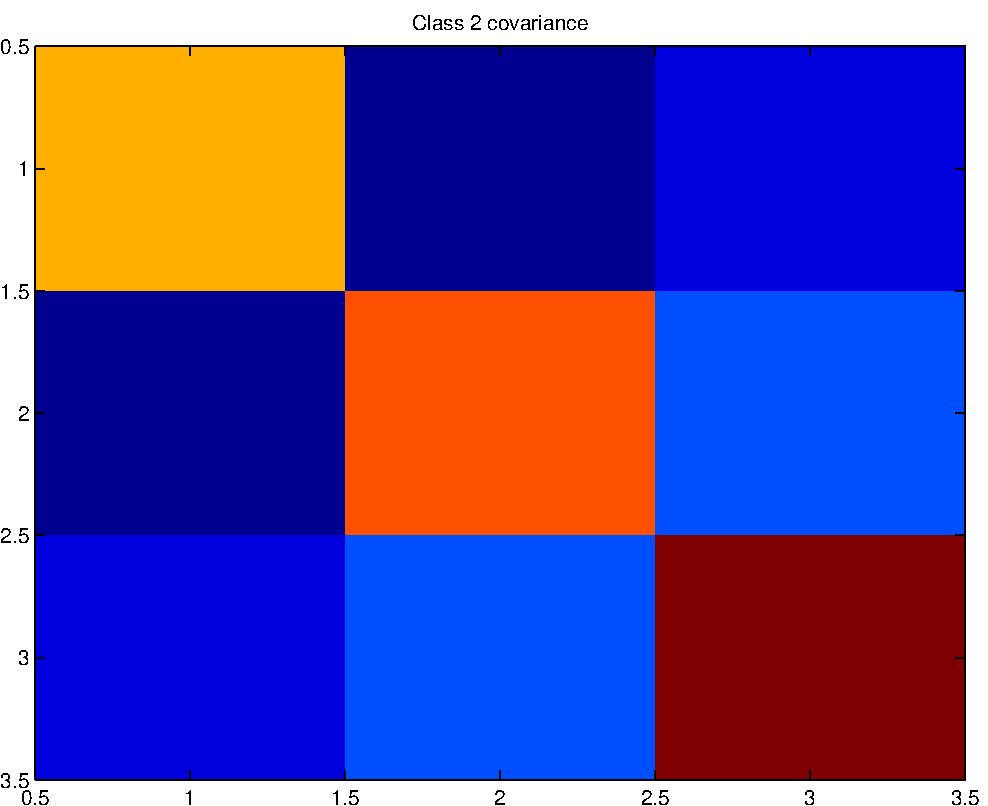
\includegraphics[width=10.0cm,height=10.0cm]{rv2_corr.pdf}

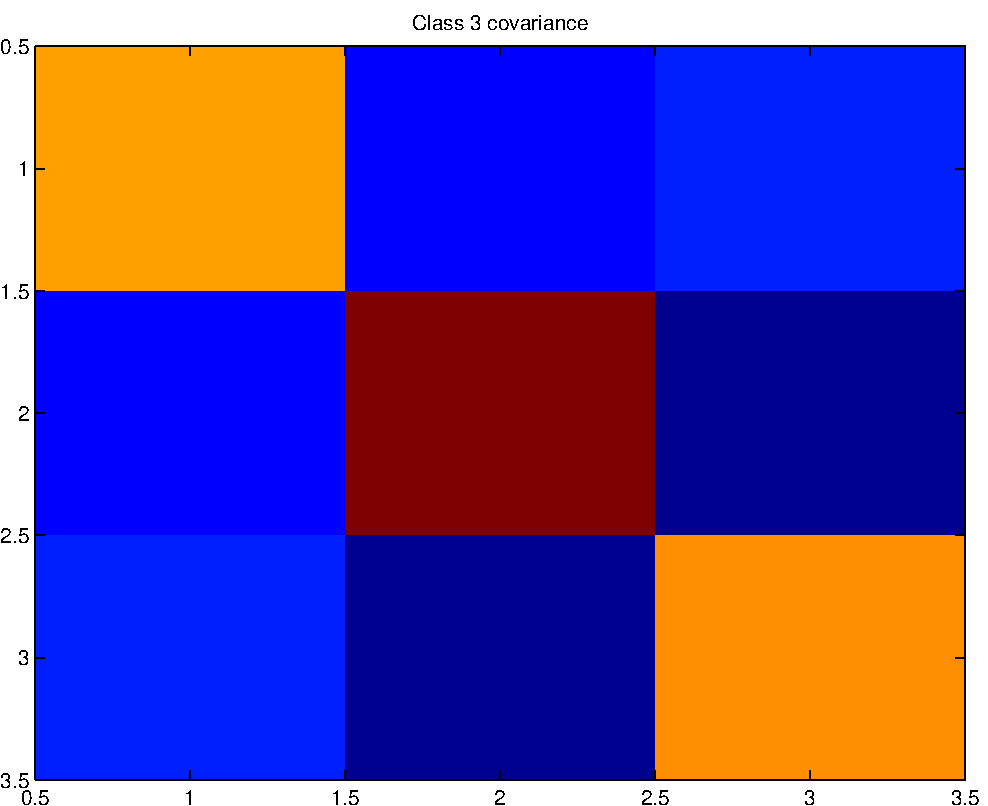
\includegraphics[width=10.0cm,height=10.0cm]{rv3_corr.pdf}

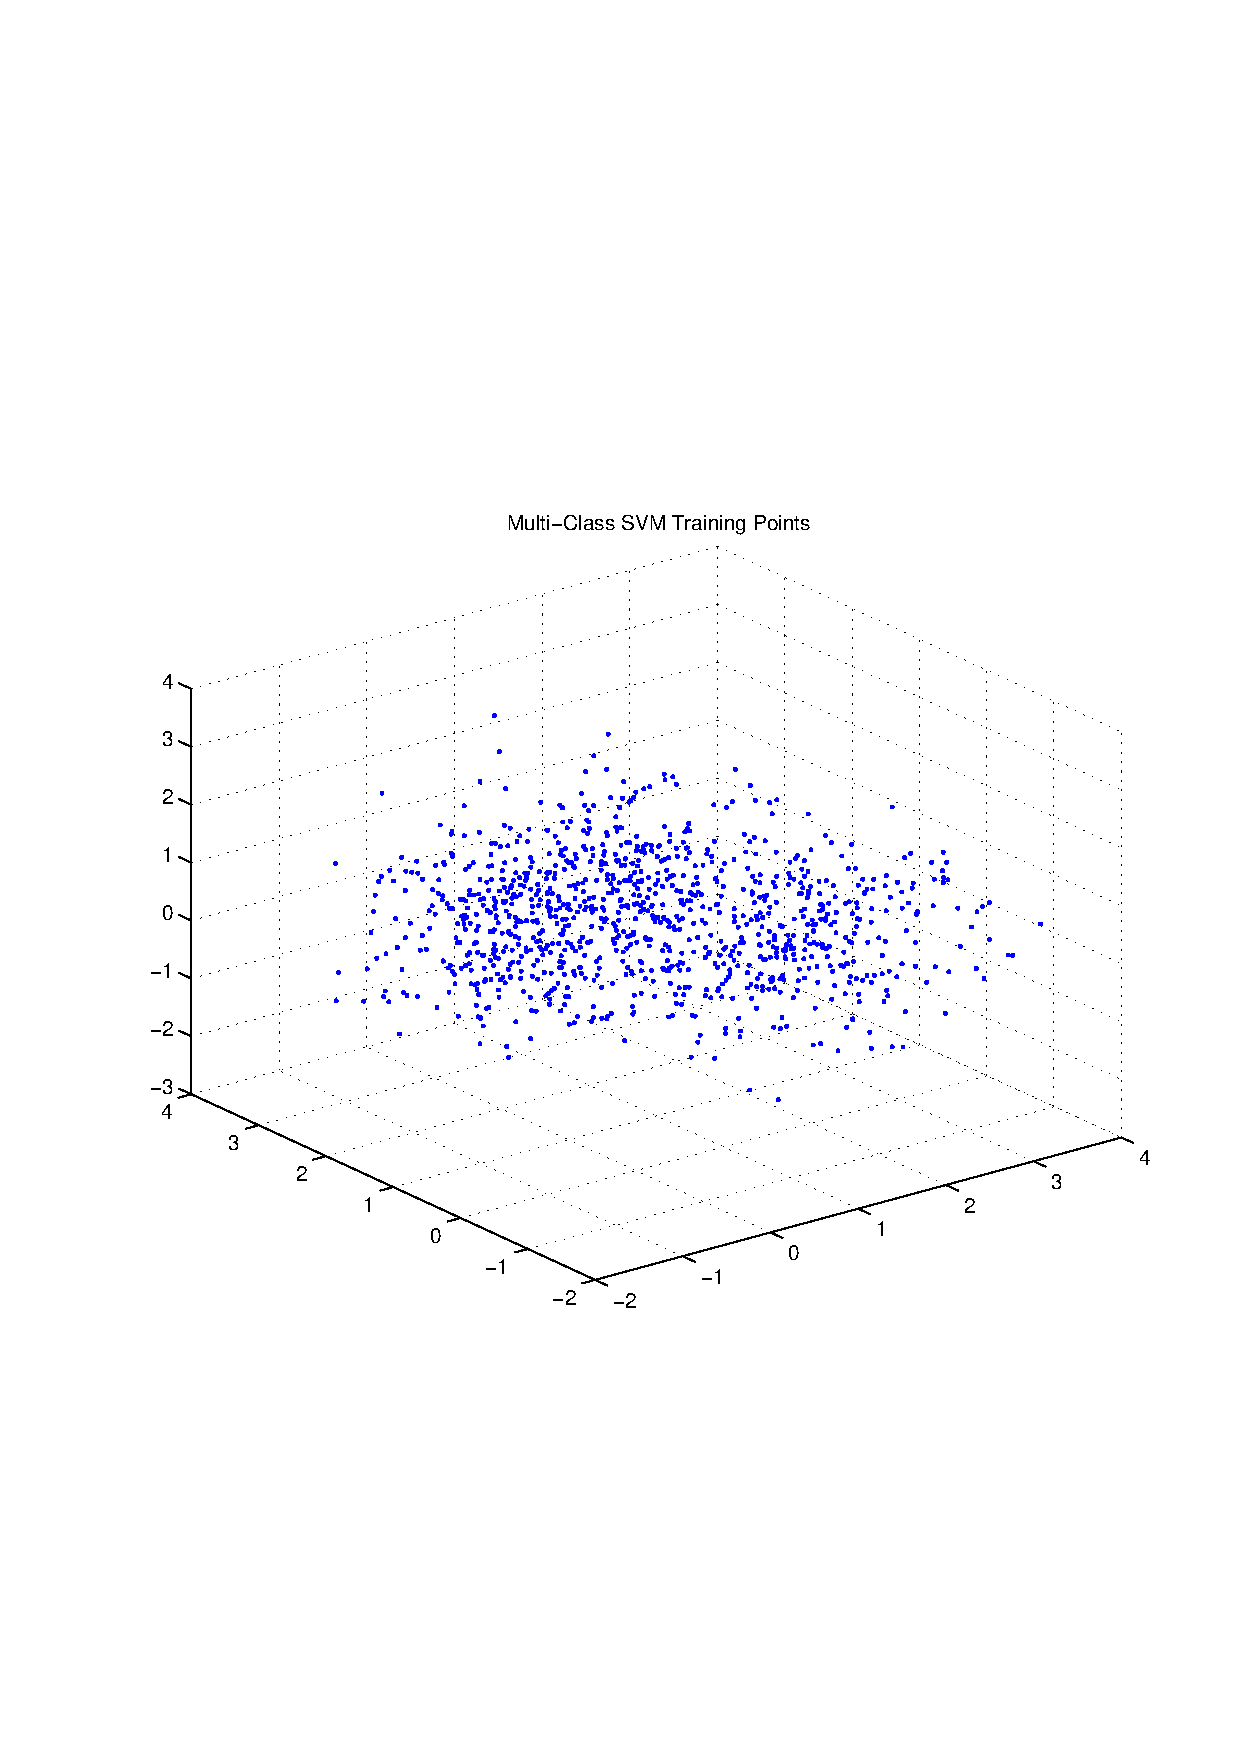
\includegraphics[width=10.0cm,height=10.0cm]{trainingPoints.pdf}

These are the SVM parameters - the RBF kernel is used\begin{itemize}
\item allOutlierFraction=0.05
\item mixingCoeff=0.3
\item smoThresh=1.0/10000.0
\item sigma=1
\end{itemize}
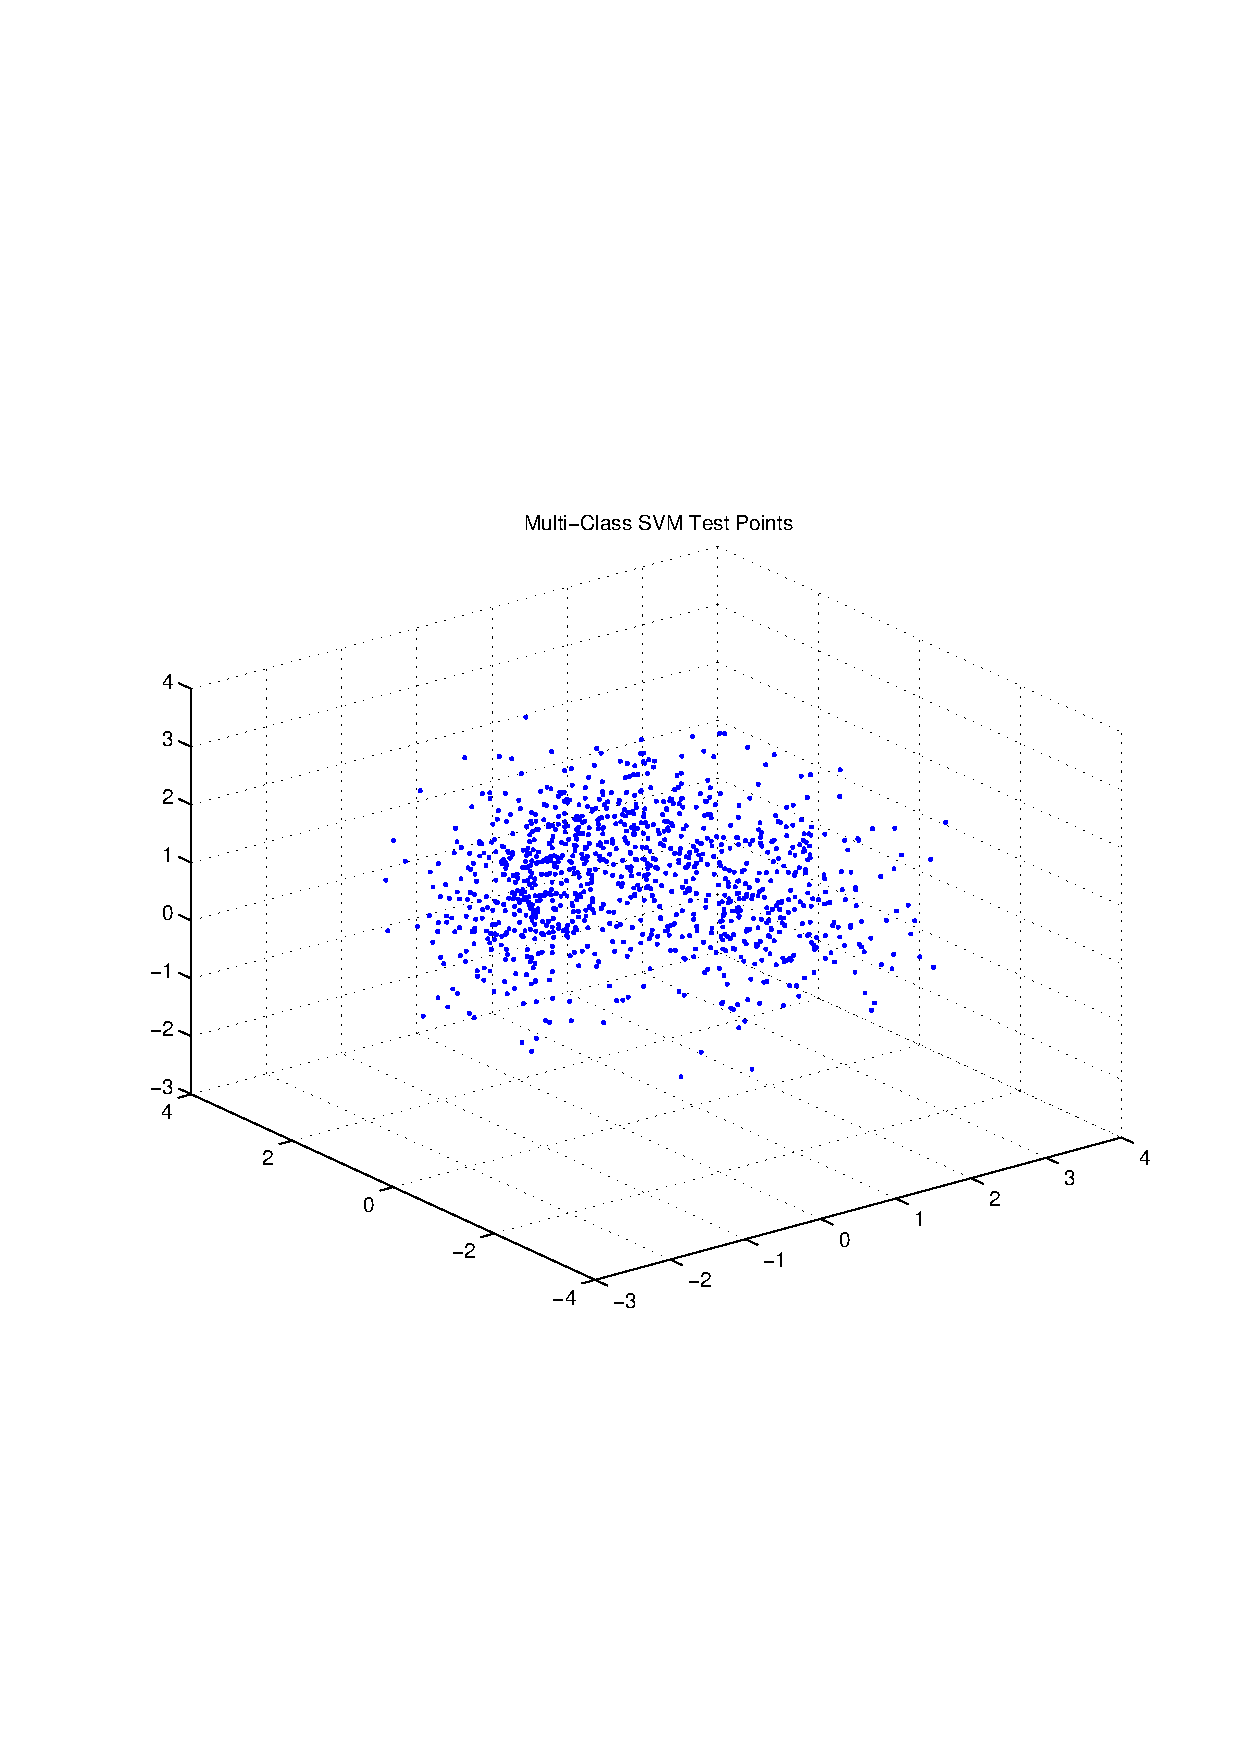
\includegraphics[width=10.0cm,height=10.0cm]{testPoints.pdf}

The marginal sample moments (mean var skew kurtosis) for training points.\newline
\begin{tabular}{ c |  c  c  c  c}
Feature & $\mu_1$ & $\mu_2$ & $\mu_3$ & $\mu_4$ \\
0 & +0.671 & +1.385 & +0.441& +2.578 \\
\hline
1 & +0.705 & +1.284 & +0.325& +2.387 \\
\hline
2 & +0.707 & +1.348 & +0.546& +2.755 \\
\hline
\end{tabular}
\newline
The marginal sample moments (mean var skew kurtosis) for test points.\newline
\begin{tabular}{ c | c  c  c  c}
Feature & $\mu_1$ & $\mu_2$ & $\mu_3$ & $\mu_4$ \\
0 & +0.679 & +1.293 & +0.617& +2.733\\
\hline
1 & +0.671 & +1.284 & +0.359& +2.428\\
\hline
2 & +0.726 & +1.260 & +0.548& +2.621\\
\hline
\end{tabular}\newline
\includegraphics[width=10.0cm,height=10.0cm]{classDiffs.pdf}

The error rate for this run is +0.203\newline
QueryPerformanceCounter  =  +5.782
\subsubsection{Matrix Quick Check <double>}
QueryPerformanceCounter  =  +0.093
\subsubsection{Linear Regression atan data 3x1}
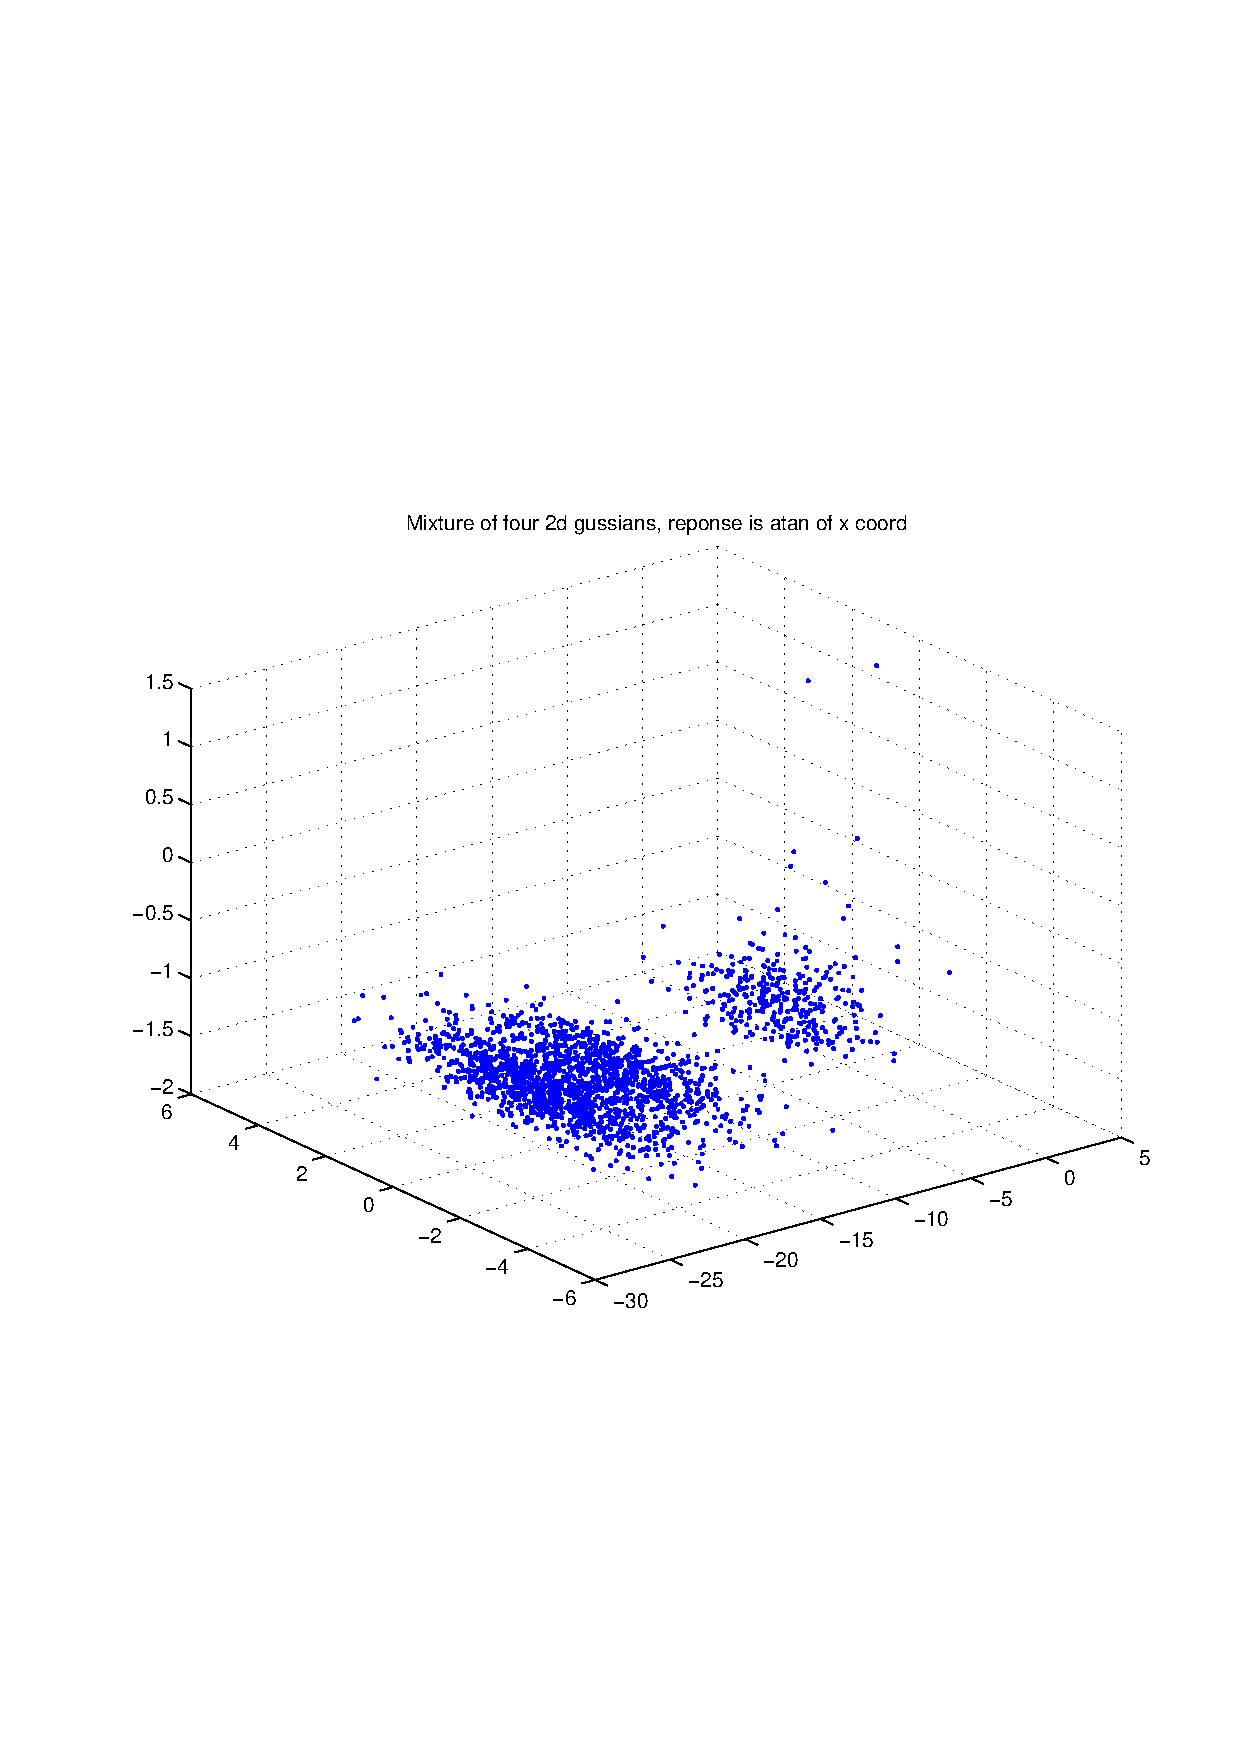
\includegraphics[width=10.0cm,height=10.0cm]{AtanDataSet.pdf}

\subsubsection{3 x 1 Linear Regression}
Sample size = 4000

Number of features = 3

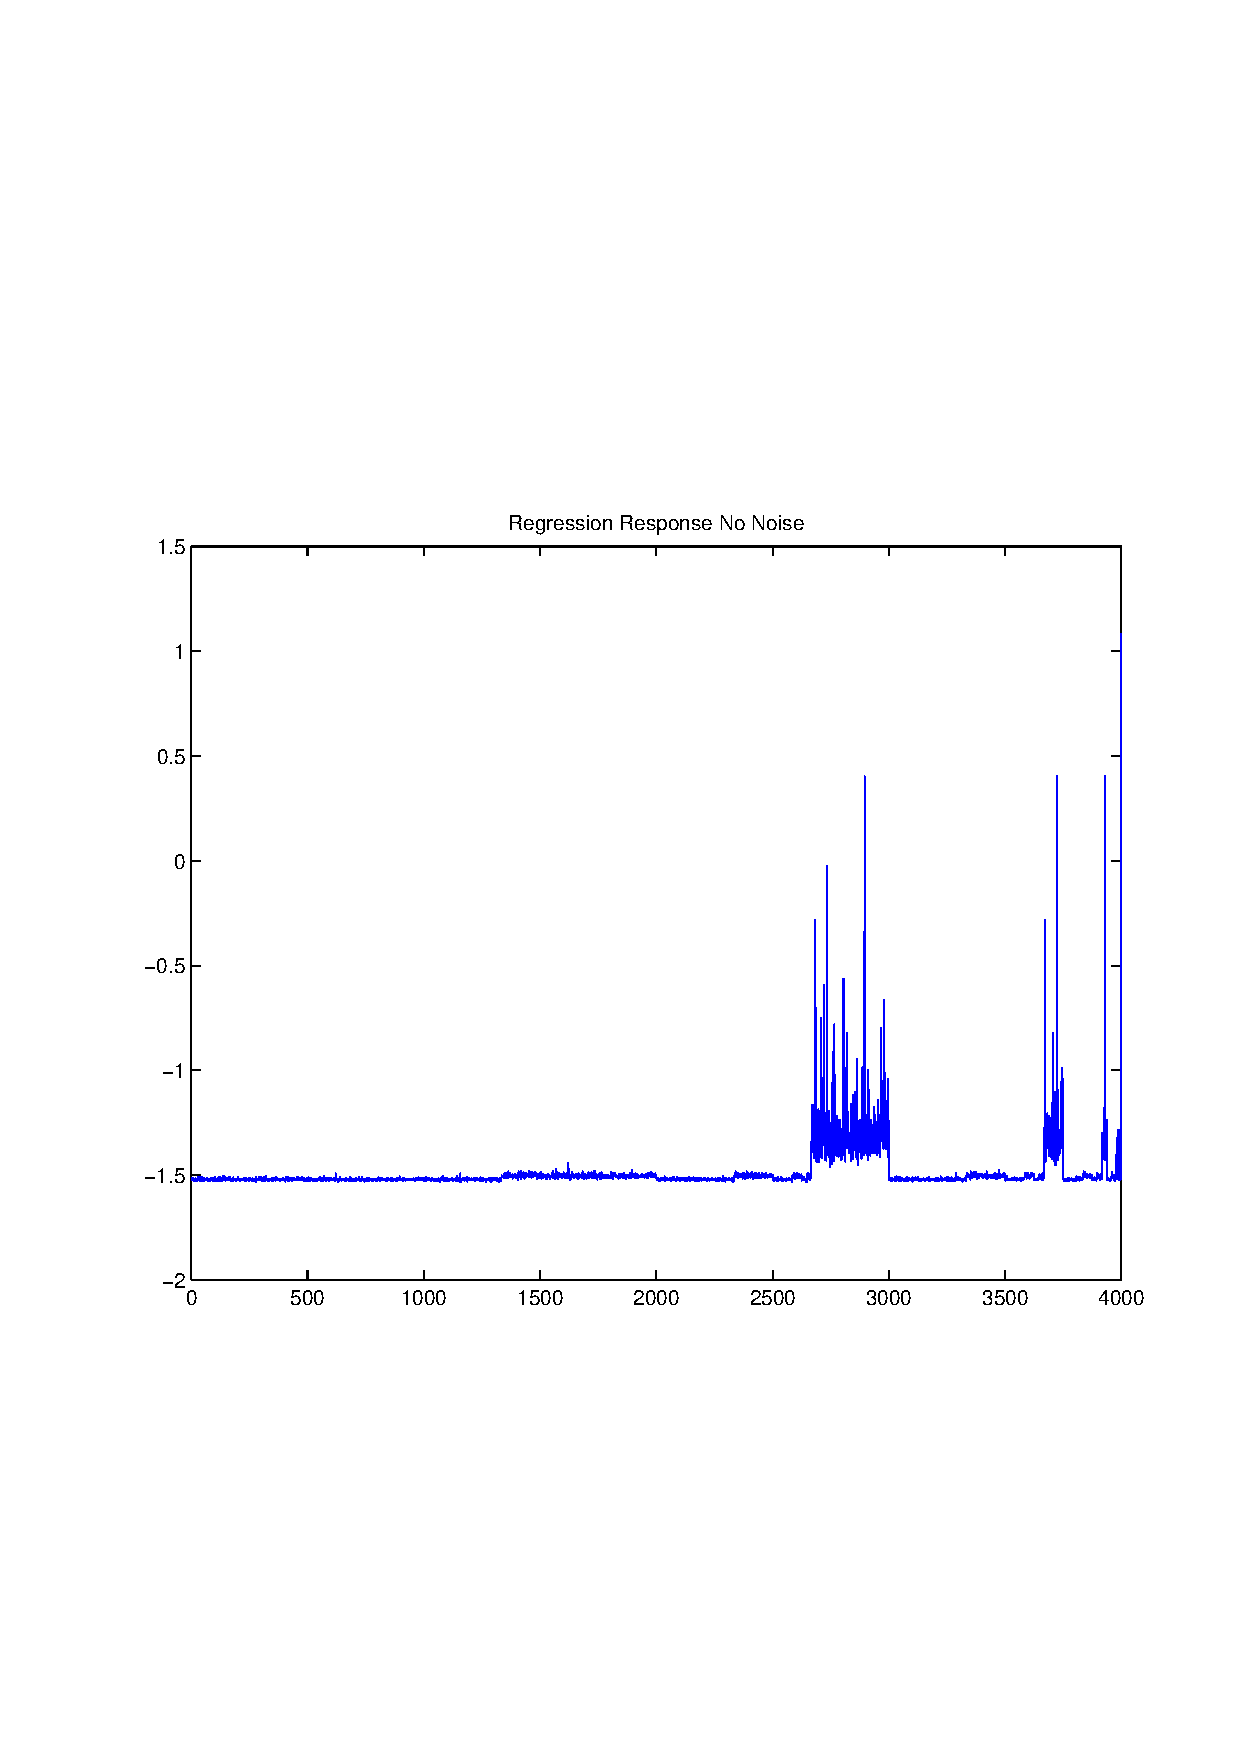
\includegraphics[width=10.0cm,height=10.0cm]{AtanDataSet_regression_response_no_noise.pdf}

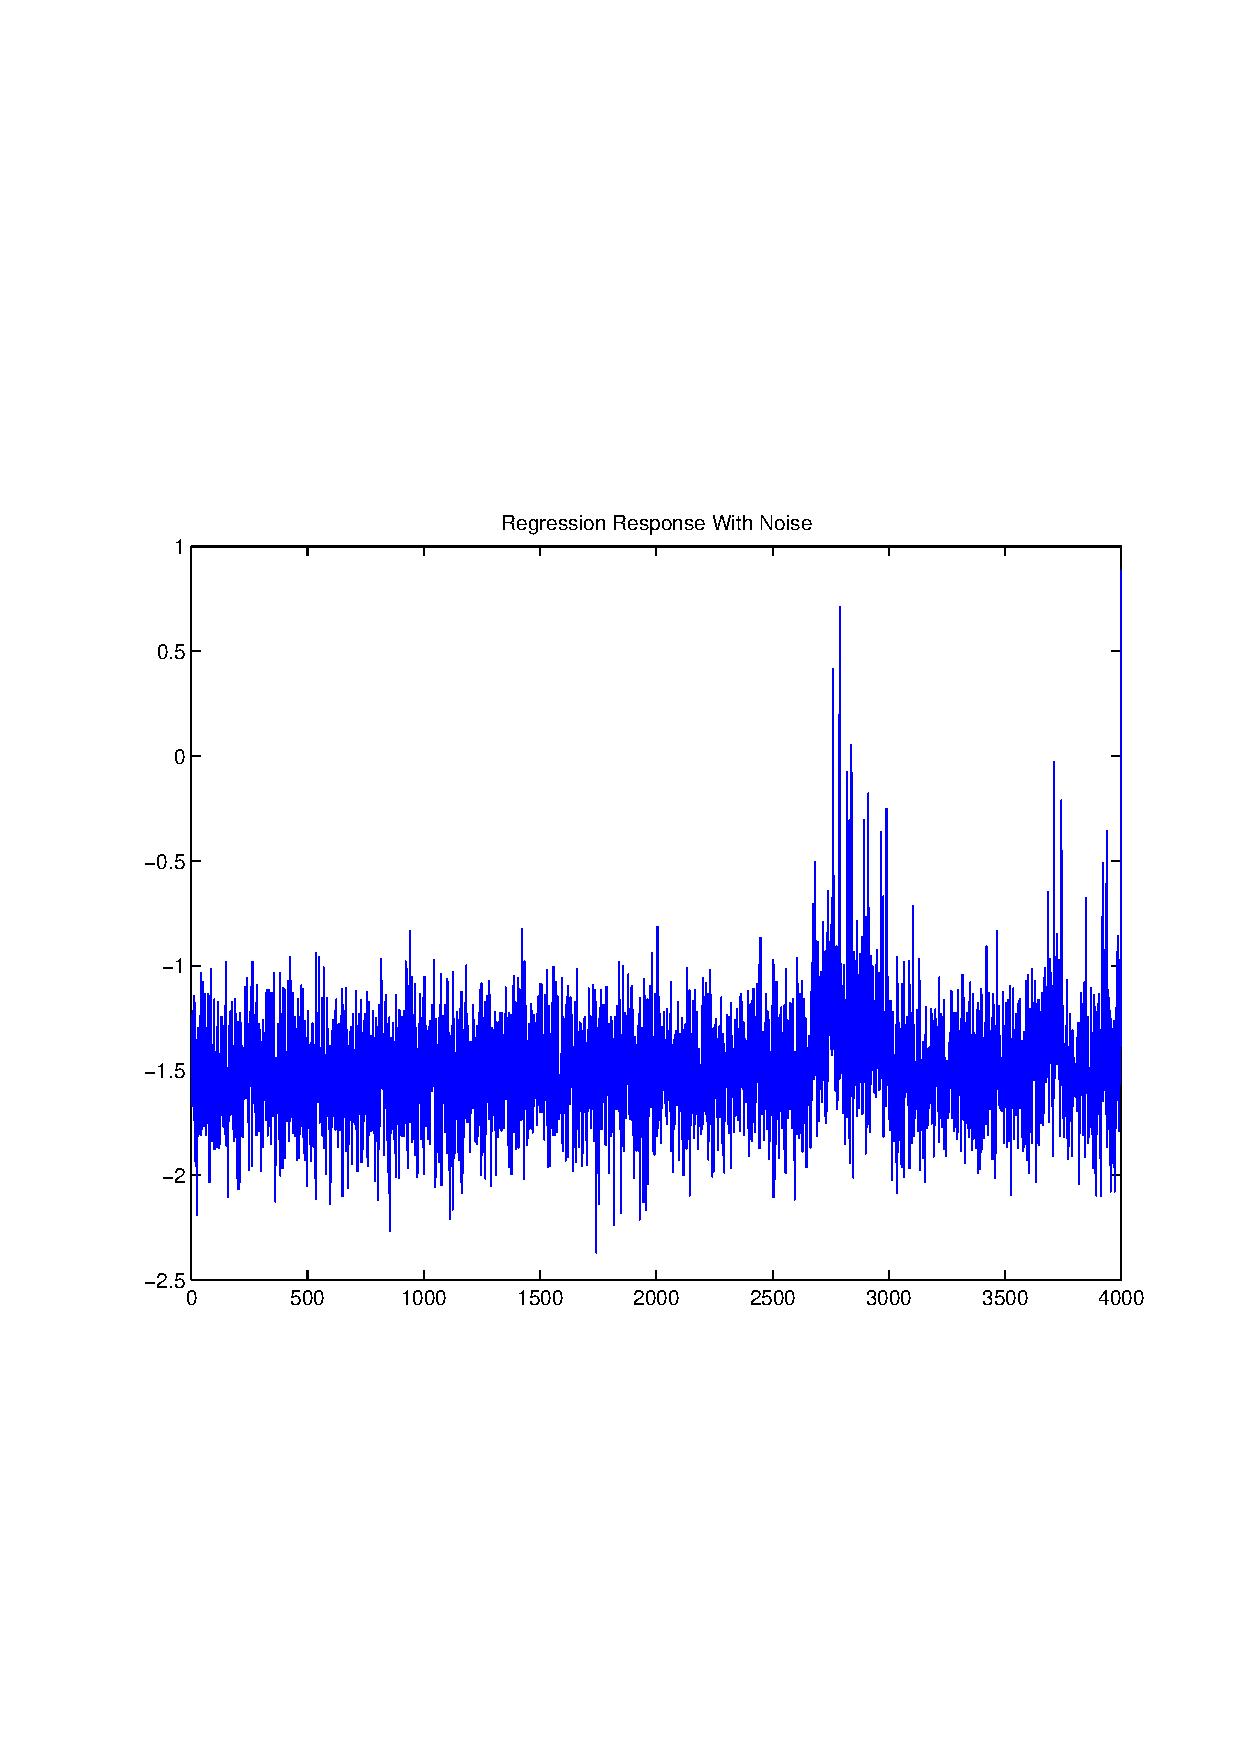
\includegraphics[width=10.0cm,height=10.0cm]{AtanDataSet_regression_response_with_noise.pdf}

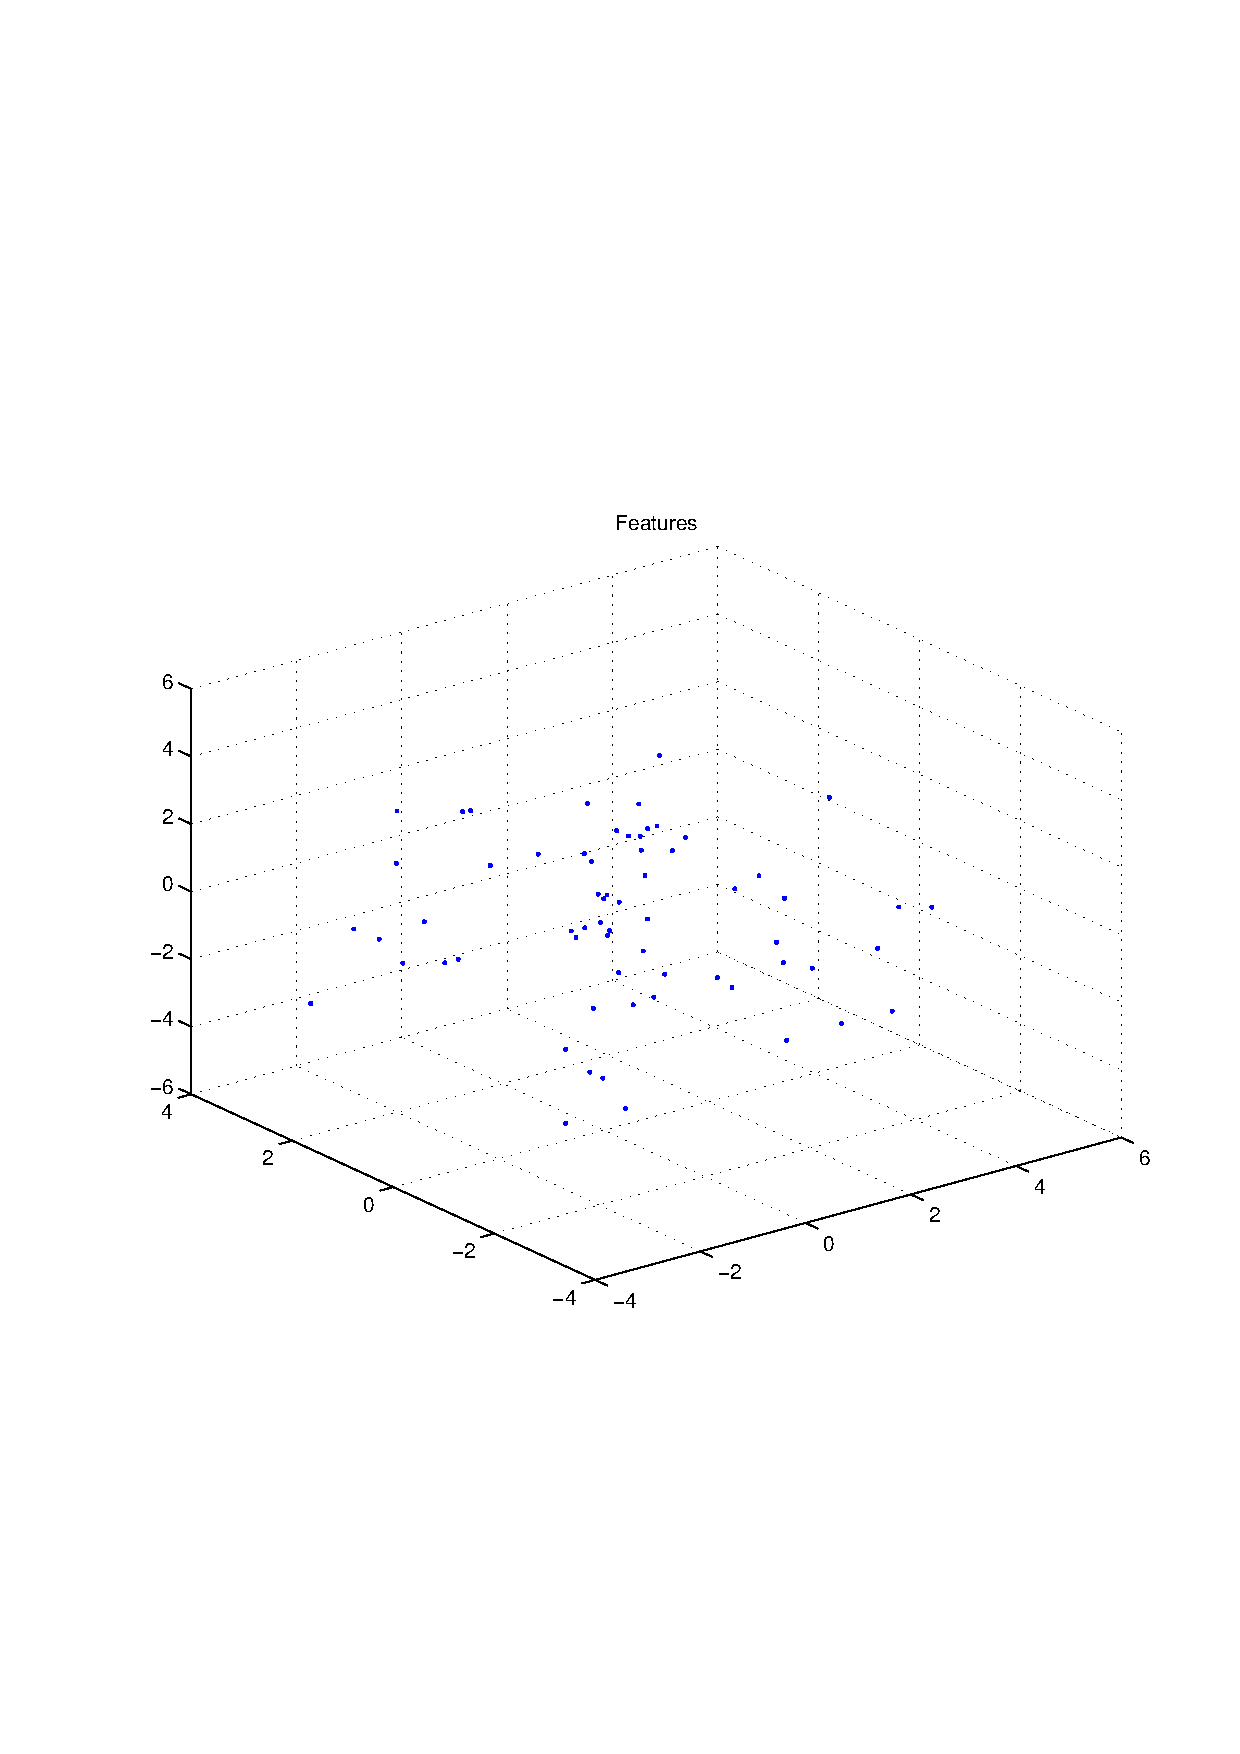
\includegraphics[width=10.0cm,height=10.0cm]{regression_features.pdf}

Response
-1.436
-1.669
-1.577
-1.238
-1.309
-1.347
-1.407
-1.287
-1.318
-1.143
-1.668
-1.379
-1.746
-1.505
-1.435
-1.931
-1.174
-1.376
-1.958
-1.597
-1.435
-1.537
-1.355
-1.865
-1.478
-2.189
-1.304
-1.387
-1.460
-1.769
-1.587
-1.353
-1.813
-1.801
-1.684
-1.241
-1.265
-1.497
-1.352
-1.811
-1.167
-1.380
-1.020
-1.258
-1.226
-1.767
-1.521
-1.701
-1.525
-1.084
-1.409
-1.283
-1.561
-1.763
-1.446
-1.671
-1.459
-1.136
-1.674
-1.681
-1.489
-1.777
-1.540
-1.651
-1.807
-1.299
-1.494
-1.711
-1.542
-1.502
-1.186
-1.125
-1.739
-1.234
-1.673
-1.848
-1.607
-2.027
-1.149
-1.596
-1.435
-1.529
-1.659
-1.034
-1.352
-1.008
-1.643
-1.500
-1.856
-1.563
-1.519
-1.397
-1.387
-1.537
-1.410
-1.583
-1.382
-1.232
-1.161
-1.883
-1.821
-1.533
-1.627
-1.837
-1.694
-1.838
-1.409
-1.500
-1.618
-1.631
-1.872
-1.440
-1.173
-1.379
-1.754
-1.609
-1.813
-1.420
-1.878
-1.556
-1.671
-1.622
-1.851
-1.733
-1.806
-1.554
-1.712
-1.452
-1.409
-1.245
-1.687
-1.606
-1.701
-1.664
-1.543
-1.525
-1.576
-1.770
-1.721
-1.413
-1.671
-1.469
-1.292
-1.773
-1.797
-1.187
-1.729
-0.985
-1.637
-1.780
-1.862
-1.532
-1.486
-1.723
-1.573
-1.643
-1.676
-1.488
-2.113
-1.710
-1.377
-1.308
-1.282
-1.427
-1.686
-1.602
-1.336
-1.224
-1.716
-1.503
-1.381
-1.478
-1.375
-1.189
-1.173
-1.529
-1.629
-1.773
-1.491
-1.386
-1.494
-1.591
-1.835
-1.599
-1.482
-1.824
-1.158
-1.226
-1.561
-1.441
-1.754
-1.241
-1.737
-1.383
-1.478
-1.424
-2.017
-1.406
-1.554
-1.631
-1.266
-1.357
-2.059
-1.755
-1.349
-1.411
-2.038
-1.403
-1.464
-1.230
-1.544
-1.275
-1.616
-1.737
-1.272
-1.395
-1.515
-1.814
-1.731
-1.523
-1.817
-1.436
-1.613
-1.497
-1.449
-1.392
-1.645
-1.543
-1.539
-1.098
-1.451
-1.391
-1.398
-1.173
-1.620
-1.627
-1.518
-1.443
-1.410
-1.057
-1.484
-1.538
-1.654
-1.628
-1.327
-1.745
-1.285
-1.449
-1.963
-1.517
-1.517
-1.433
-1.438
-1.368
-1.087
-1.555
-1.332
-1.575
-1.336
-1.958
-1.958
-1.472
-0.987
-1.323
-1.664
-1.192
-1.370
-1.236
-1.571
-1.638
-1.498
-1.256
-1.630
-1.437
-1.710
-1.438
-1.201
-1.740
-1.174
-1.811
-1.347
-1.462
-1.089
-1.802
-1.645
-1.591
-1.703
-1.559
-1.513
-1.366
-1.298
-1.780
-1.429
-1.302
-1.568
-1.507
-1.428
-1.485
-1.978
-1.972
-1.374
-1.457
-1.581
-1.541
-1.680
-1.605
-1.249
-1.858
-1.451
-1.746
-1.319
-1.443
-1.639
-1.320
-1.539
-1.573
-1.588
-1.514
-1.412
-1.132
-1.504
-1.517
-1.717
-1.408
-1.115
-1.584
-1.588
-1.813
-1.415
-1.602
-1.599
-1.418
-1.423
-1.569
-1.119
-1.658
-1.422
-1.210
-1.759
-1.287
-1.417
-1.183
-1.853
-1.320
-1.110
-1.625
-1.644
-1.713
-1.412
-1.439
-1.710
-1.364
-1.473
-1.257
-1.027
-1.093
-1.602
-1.481
-1.564
-1.497
-2.124
-1.442
-1.947
-1.525
-1.458
-1.678
-1.479
-1.620
-1.620
-1.689
-1.280
-1.496
-1.518
-1.697
-1.574
-1.467
-1.577
-1.737
-1.830
-1.038
-1.857
-1.378
-2.006
-1.801
-1.596
-1.618
-1.222
-1.716
-1.247
-1.368
-1.374
-1.964
-1.776
-1.117
-1.696
-1.285
-1.615
-1.875
-1.602
-1.372
-1.101
-1.620
-1.580
-1.925
-1.676
-1.556
-1.658
-1.541
-1.594
-1.475
-1.746
-1.415
-1.500
-1.445
-1.613
-1.297
-1.076
-1.330
-1.313
-1.520
-1.501
-1.835
-1.603
-1.247
-0.947
-1.586
-1.070
-1.717
-1.261
-1.442
-1.412
-1.194
-1.169
-1.376
-1.131
-1.557
-1.804
-1.681
-1.499
-1.397
-1.571
-1.597
-1.685
-1.307
-1.247
-1.404
-1.812
-1.304
-1.322
-1.462
-1.395
-1.321
-1.833
-1.632
-1.509
-1.947
-1.157
-1.238
-1.343
-1.623
-1.900
-1.555
-1.916
-1.784
-1.248
-1.744
-1.807
-1.536
-1.538
-1.196
-1.424
-1.661
-1.082
-1.170
-1.670
-1.774
-1.383
-1.124
-1.536
-1.797
-1.235
-1.711
-1.888
-1.341
-1.722
-1.526
-1.407
-1.257
-1.931
-1.458
-1.627
-1.536
-1.491
-1.521
-1.355
-1.442
-2.052
-1.337
-1.801
-1.607
-1.224
-1.286
-1.735
-1.497
-1.783
-1.583
-1.382
-1.520
-1.849
-1.400
-1.551
-1.511
-1.825
-1.630
-1.367
-1.929
-1.768
-1.526
-1.377
-1.412
-1.270
-1.797
-1.483
-1.758
-1.865
-1.764
-1.839
-1.466
-1.375
-1.500
-1.383
-2.019
-1.404
-1.495
-0.935
-1.568
-2.117
-1.332
-1.392
-1.218
-1.420
-1.306
-1.441
-1.656
-1.492
-1.446
-1.527
-1.423
-1.467
-0.956
-1.319
-1.720
-1.748
-1.540
-1.636
-1.482
-1.624
-1.383
-1.436
-1.448
-1.453
-1.159
-1.824
-1.543
-1.732
-1.458
-1.497
-1.616
-1.014
-1.554
-1.627
-1.501
-1.875
-1.668
-1.427
-1.832
-1.543
-1.559
-1.689
-1.641
-1.992
-1.339
-1.148
-1.691
-1.506
-1.542
-1.659
-1.400
-1.298
-1.474
-1.423
-1.779
-1.486
-1.598
-1.513
-1.374
-1.856
-2.136
-1.895
-1.531
-1.724
-1.520
-1.402
-1.730
-1.753
-1.306
-1.352
-1.620
-1.729
-1.261
-1.659
-1.659
-1.395
-1.439
-1.659
-1.304
-1.227
-1.504
-1.470
-1.781
-1.184
-1.282
-1.161
-1.190
-1.528
-1.348
-1.364
-1.541
-1.308
-1.869
-1.743
-1.640
-1.287
-1.682
-1.281
-1.285
-1.462
-1.774
-1.447
-1.356
-1.772
-1.271
-1.227
-1.307
-1.512
-1.761
-1.736
-1.115
-2.094
-1.272
-1.529
-1.633
-1.196
-2.097
-1.225
-1.547
-1.433
-1.564
-1.692
-1.593
-1.443
-1.711
-1.385
-1.890
-1.112
-1.296
-1.736
-1.308
-1.315
-1.625
-1.695
-1.666
-1.446
-1.769
-2.063
-1.576
-1.824
-1.842
-1.762
-1.391
-1.636
-1.668
-1.494
-1.321
-1.460
-1.425
-1.342
-1.296
-1.742
-1.486
-1.363
-1.306
-1.939
-1.240
-1.511
-1.657
-1.441
-1.734
-1.754
-1.725
-1.409
-1.566
-1.749
-1.619
-1.416
-1.404
-1.492
-1.119
-1.785
-1.408
-1.653
-1.582
-1.726
-1.392
-1.976
-1.841
-1.402
-1.675
-1.292
-1.709
-1.496
-1.307
-1.218
-1.474
-1.521
-1.418
-1.611
-1.715
-1.287
-1.539
-1.160
-1.941
-1.532
-1.424
-1.315
-1.530
-1.540
-1.599
-1.711
-1.874
-1.328
-1.748
-1.518
-1.433
-1.266
-1.573
-1.507
-1.237
-1.460
-1.400
-1.224
-1.551
-1.431
-1.912
-1.302
-1.129
-1.532
-1.850
-1.511
-1.962
-1.330
-1.647
-1.433
-1.806
-1.184
-1.651
-1.775
-1.457
-1.546
-1.670
-1.338
-1.696
-1.779
-1.525
-1.678
-1.693
-1.737
-1.431
-1.747
-1.220
-1.319
-1.798
-1.585
-1.344
-1.815
-1.506
-1.559
-1.537
-2.018
-1.472
-1.649
-1.752
-1.645
-1.709
-1.261
-1.749
-1.521
-1.294
-1.458
-1.841
-1.416
-1.801
-2.107
-1.877
-1.418
-1.651
-1.373
-1.872
-1.182
-1.198
-1.299
-1.765
-1.581
-1.584
-0.973
-1.500
-1.341
-1.395
-1.548
-1.328
-1.075
-1.500
-1.522
-1.383
-1.474
-1.326
-1.797
-1.508
-1.558
-1.910
-1.521
-1.455
-1.185
-1.470
-1.471
-1.492
-1.150
-1.308
-1.497
-1.846
-1.443
-1.278
-1.632
-1.629
-1.984
-1.325
-1.500
-1.544
-2.087
-1.585
-1.812
-1.251
-1.624
-1.594
-2.265
-1.737
-1.791
-1.424
-1.342
-1.645
-1.535
-1.756
-1.791
-1.602
-1.479
-1.309
-1.690
-1.280
-1.653
-1.826
-1.540
-1.459
-1.676
-1.368
-1.672
-1.902
-1.690
-1.510
-1.807
-1.553
-2.002
-1.149
-1.510
-1.756
-1.345
-1.408
-1.634
-1.683
-1.658
-1.315
-1.503
-1.284
-1.570
-1.212
-2.011
-1.431
-1.459
-1.222
-1.688
-1.294
-1.806
-1.633
-1.285
-1.284
-1.814
-1.796
-1.254
-1.613
-1.594
-1.382
-1.750
-1.480
-1.299
-1.218
-1.807
-1.470
-1.548
-1.494
-1.745
-1.725
-1.391
-0.980
-1.608
-1.226
-1.577
-1.437
-1.019
-1.688
-1.879
-1.709
-1.957
-1.791
-1.750
-1.598
-1.315
-1.472
-1.102
-1.405
-1.407
-1.719
-0.836
-1.745
-1.383
-1.416
-1.555
-1.557
-1.054
-1.604
-1.515
-1.456
-1.841
-1.517
-1.397
-1.240
-1.350
-1.292
-1.827
-1.685
-1.466
-1.560
-1.894
-1.088
-1.601
-1.300
-1.678
-1.325
-1.780
-1.313
-1.692
-1.397
-2.019
-1.814
-1.599
-1.732
-1.466
-1.993
-1.559
-1.659
-1.340
-1.498
-1.279
-1.444
-1.574
-1.535
-1.141
-1.268
-1.824
-1.587
-1.487
-1.438
-1.457
-1.569
-1.348
-1.395
-1.873
-1.358
-1.606
-1.199
-1.111
-1.577
-1.994
-1.668
-1.051
-1.742
-1.608
-1.605
-1.282
-1.409
-1.789
-1.333
-1.603
-1.549
-1.356
-1.482
-1.323
-1.314
-1.824
-1.467
-1.549
-1.314
-1.295
-1.680
-1.352
-1.461
-1.554
-1.560
-1.857
-1.262
-1.546
-1.466
-1.524
-1.467
-1.401
-1.597
-1.192
-1.599
-1.253
-1.463
-1.219
-1.287
-1.517
-1.485
-1.573
-0.976
-1.569
-1.531
-1.630
-1.416
-2.051
-1.591
-1.798
-1.268
-1.453
-2.005
-1.727
-1.654
-1.728
-1.428
-1.560
-1.563
-1.383
-1.415
-1.480
-1.611
-1.933
-1.324
-1.246
-1.578
-1.394
-1.275
-1.322
-1.181
-1.709
-1.384
-1.036
-2.055
-1.832
-1.527
-1.406
-1.504
-1.492
-1.650
-1.239
-1.486
-1.614
-1.652
-1.587
-1.371
-1.384
-1.453
-1.189
-1.800
-1.496
-1.452
-1.610
-1.352
-1.282
-1.364
-1.782
-1.065
-1.902
-1.354
-1.320
-1.801
-1.076
-1.786
-1.368
-1.978
-1.532
-1.311
-2.204
-1.757
-1.546
-1.495
-1.789
-1.341
-1.324
-1.893
-1.575
-1.860
-1.539
-1.305
-1.684
-2.164
-1.024
-1.585
-1.064
-1.507
-1.800
-1.596
-1.916
-1.620
-1.496
-1.887
-1.480
-1.639
-1.413
-1.562
-1.572
-1.721
-1.374
-1.229
-1.339
-1.494
-1.650
-1.253
-1.507
-1.898
-1.398
-1.493
-1.923
-1.514
-1.353
-1.815
-1.212
-1.637
-1.651
-1.318
-1.238
-2.020
-1.764
-1.133
-1.732
-1.948
-1.745
-2.088
-1.868
-1.319
-1.603
-1.561
-1.318
-1.822
-1.476
-1.363
-1.737
-1.499
-1.183
-1.593
-1.237
-1.380
-1.596
-1.229
-0.979
-1.547
-1.333
-1.429
-1.573
-1.743
-1.533
-1.291
-1.361
-1.446
-1.636
-1.609
-1.556
-1.384
-1.734
-1.720
-1.719
-1.893
-1.362
-1.486
-1.702
-1.467
-1.453
-1.518
-1.479
-1.558
-1.520
-1.478
-1.676
-1.330
-1.182
-1.352
-1.367
-1.381
-1.615
-1.343
-1.478
-1.698
-1.661
-1.826
-1.482
-1.589
-1.775
-1.716
-1.292
-1.854
-1.290
-1.391
-1.815
-1.506
-1.451
-1.455
-1.676
-1.226
-1.526
-1.353
-1.321
-1.763
-1.174
-1.295
-1.115
-1.367
-2.002
-1.402
-1.491
-1.085
-1.544
-1.479
-1.783
-1.903
-1.623
-1.621
-1.694
-1.345
-1.259
-1.668
-1.248
-1.891
-1.680
-1.174
-1.670
-1.898
-2.010
-1.511
-1.163
-1.209
-1.456
-1.459
-1.140
-1.618
-1.652
-1.644
-1.377
-1.605
-1.594
-1.642
-1.486
-1.715
-1.088
-1.737
-1.432
-1.135
-1.326
-1.714
-1.657
-2.050
-1.496
-1.361
-1.750
-1.297
-1.394
-1.554
-1.781
-1.603
-1.562
-1.716
-1.370
-1.720
-1.537
-1.303
-1.639
-1.525
-1.611
-1.636
-1.787
-1.228
-1.995
-1.595
-1.253
-1.366
-1.509
-1.274
-1.495
-1.290
-1.462
-1.814
-1.398
-1.699
-1.728
-1.293
-1.269
-1.784
-1.756
-1.219
-1.524
-1.699
-1.675
-1.681
-1.519
-1.447
-1.784
-1.239
-1.773
-1.794
-1.562
-1.481
-1.378
-1.381
-1.645
-1.543
-1.661
-1.786
-1.374
-1.314
-1.407
-1.600
-1.262
-1.240
-1.470
-1.093
-1.641
-1.381
-1.624
-1.355
-1.369
-1.283
-1.331
-1.246
-1.512
-1.668
-1.349
-1.853
-1.962
-1.240
-1.837
-1.674
-1.538
-1.607
-1.849
-1.450
-1.531
-1.225
-1.334
-1.356
-1.979
-1.704
-1.408
-1.533
-1.633
-1.110
-1.512
-1.307
-1.542
-1.331
-1.773
-1.041
-1.174
-1.187
-1.647
-1.562
-1.547
-1.332
-1.872
-1.330
-1.330
-1.627
-1.171
-1.811
-1.182
-1.425
-1.580
-1.592
-1.057
-1.818
-1.850
-1.235
-1.680
-1.359
-1.117
-1.491
-1.358
-1.106
-1.568
-1.419
-1.743
-1.152
-1.552
-1.551
-1.356
-1.454
-1.286
-0.822
-1.297
-1.555
-1.640
-1.513
-1.721
-1.230
-2.002
-1.498
-0.981
-1.355
-1.417
-1.377
-1.695
-1.514
-1.206
-1.604
-1.373
-1.846
-1.389
-1.344
-1.440
-1.497
-1.823
-1.366
-1.757
-1.730
-1.473
-1.785
-1.277
-1.579
-1.490
-1.448
-1.637
-1.788
-1.491
-1.169
-1.711
-1.513
-1.207
-1.802
-1.471
-1.426
-1.677
-1.796
-1.327
-1.301
-1.630
-1.249
-1.605
-1.687
-1.569
-1.287
-1.428
-1.654
-1.288
-1.526
-1.293
-1.260
-1.520
-1.434
-1.757
-1.429
-1.343
-1.214
-1.513
-1.480
-1.309
-1.563
-1.138
-1.344
-1.641
-1.696
-1.275
-1.537
-1.594
-1.708
-1.408
-1.097
-1.510
-1.166
-1.231
-1.600
-1.103
-1.547
-1.691
-1.243
-1.411
-1.655
-1.628
-1.539
-1.374
-1.459
-1.533
-1.823
-1.554
-1.494
-1.134
-1.352
-1.167
-1.654
-1.643
-1.592
-1.386
-1.023
-1.400
-1.499
-1.768
-1.434
-1.963
-1.367
-1.346
-1.846
-1.559
-1.174
-1.634
-1.691
-1.297
-1.548
-1.428
-1.960
-1.369
-1.611
-1.494
-1.384
-1.765
-1.339
-1.176
-1.632
-1.178
-1.423
-1.182
-1.421
-1.801
-0.986
-1.768
-1.462
-1.571
-1.587
-1.832
-1.747
-1.104
-1.279
-1.320
-1.077
-1.415
-1.479
-1.793
-1.454
-1.578
-1.630
-1.622
-1.142
-1.304
-1.276
-1.503
-1.636
-1.725
-1.682
-1.530
-1.511
-1.674
-1.692
-1.651
-1.554
-1.422
-1.490
-1.717
-1.424
-1.836
-1.088
-1.368
-1.784
-1.614
-1.242
-1.882
-1.510
-1.709
-1.368
-1.638
-1.594
-1.303
-1.537
-1.698
-1.598
-1.272
-1.932
-1.195
-1.380
-1.547
-1.468
-1.712
-1.721
-1.168
-1.478
-1.498
-1.265
-1.907
-1.124
-1.451
-1.623
-1.634
-1.453
-1.676
-1.524
-1.553
-1.495
-1.168
-1.469
-1.502
-1.198
-1.586
-1.225
-1.353
-1.337
-1.308
-1.510
-1.968
-1.742
-1.545
-1.488
-1.437
-1.656
-1.835
-1.874
-1.516
-1.589
-1.380
-1.167
-1.621
-1.425
-1.950
-1.561
-1.791
-1.591
-1.718
-1.015
-1.392
-1.404
-1.766
-1.414
-1.685
-1.876
-1.320
-1.734
-1.736
-1.256
-1.677
-1.261
-1.282
-1.621
-1.442
-1.278
-1.496
-1.653
-1.453
-1.972
-1.634
-1.326
-1.494
-1.901
-1.733
-1.495
-1.528
-1.257
-1.598
-1.341
-1.305
-1.643
-1.679
-1.266
-1.319
-1.752
-1.719
-1.768
-1.701
-1.951
-1.450
-1.523
-1.567
-1.349
-1.689
-1.629
-1.650
-1.550
-1.120
-1.359
-1.528
-1.562
-1.489
-1.225
-1.672
-1.273
-1.576
-1.247
-1.781
-1.341
-1.279
-1.338
-1.306
-1.273
-1.700
-1.183
-1.477
-1.092
-1.559
-1.276
-1.209
-1.844
-1.694
-1.660
-1.100
-1.579
-1.453
-1.625
-1.548
-1.167
-1.953
-2.379
-1.328
-1.452
-1.771
-1.997
-1.661
-1.545
-1.550
-1.727
-1.649
-1.705
-2.121
-2.002
-1.311
-1.211
-1.557
-1.497
-1.433
-1.788
-1.392
-1.117
-1.630
-1.424
-1.713
-1.752
-1.653
-1.785
-1.368
-1.637
-1.470
-1.242
-1.171
-1.193
-1.357
-1.377
-1.638
-1.575
-1.300
-1.442
-1.848
-1.620
-1.864
-1.423
-1.217
-1.115
-1.440
-1.449
-1.510
-1.437
-1.616
-1.519
-1.367
-1.445
-1.383
-1.288
-1.987
-1.320
-1.744
-1.599
-1.669
-1.476
-1.562
-1.576
-1.826
-1.257
-1.532
-1.478
-1.370
-1.787
-1.266
-1.526
-1.432
-1.657
-1.794
-1.349
-1.644
-1.876
-2.232
-1.448
-1.546
-1.339
-1.637
-1.233
-1.351
-1.679
-1.570
-1.417
-1.658
-1.201
-1.433
-1.255
-1.676
-1.629
-1.533
-1.561
-1.706
-0.997
-1.699
-1.724
-1.263
-1.157
-1.476
-1.777
-1.676
-1.713
-1.583
-2.181
-1.342
-1.326
-1.820
-1.713
-1.485
-1.409
-1.569
-0.997
-1.849
-1.525
-1.256
-1.452
-1.888
-1.734
-1.327
-1.232
-1.550
-1.419
-1.471
-1.666
-1.273
-1.425
-1.730
-1.539
-1.347
-1.247
-1.290
-1.268
-1.508
-1.459
-1.314
-1.061
-1.580
-1.446
-1.713
-1.209
-1.520
-1.346
-1.725
-1.570
-1.505
-1.095
-1.329
-1.672
-1.455
-1.740
-1.325
-1.469
-1.091
-1.812
-1.512
-1.226
-1.227
-1.726
-1.782
-1.820
-2.014
-1.579
-1.498
-1.423
-1.614
-1.344
-1.472
-1.874
-1.383
-1.648
-1.873
-1.394
-1.625
-1.666
-1.611
-1.301
-1.339
-1.694
-1.359
-1.201
-1.388
-1.689
-1.889
-1.542
-2.210
-1.154
-1.580
-1.501
-1.710
-1.387
-1.567
-1.634
-1.369
-1.281
-1.798
-1.463
-1.695
-1.620
-1.675
-1.499
-2.125
-1.471
-1.344
-1.063
-1.316
-1.256
-1.289
-1.158
-1.377
-1.624
-1.397
-1.439
-2.161
-1.831
-1.622
-1.257
-1.267
-1.159
-2.051
-1.627
-1.230
-1.702
-1.686
-1.630
-1.275
-1.308
-1.115
-1.389
-1.511
-1.317
-1.357
-1.514
-1.668
-1.385
-1.554
-1.465
-0.943
-1.582
-1.297
-1.777
-1.422
-1.730
-1.875
-1.762
-1.496
-1.387
-1.351
-1.904
-1.304
-1.320
-1.453
-1.135
-1.463
-1.444
-1.180
-1.689
-1.284
-1.810
-1.759
-1.571
-0.818
-1.515
-0.918
-1.534
-1.771
-1.374
-1.526
-1.671
-1.152
-1.340
-1.401
-1.410
-1.740
-1.343
-1.294
-1.686
-1.666
-1.836
-1.443
-1.639
-1.544
-1.498
-1.541
-1.455
-1.289
-1.598
-1.460
-1.222
-1.588
-1.433
-1.363
-1.531
-1.553
-1.660
-1.375
-1.402
-1.449
-1.715
-1.634
-1.684
-1.752
-1.292
-1.207
-1.507
-1.436
-1.459
-1.630
-1.437
-1.308
-1.603
-1.434
-1.543
-1.453
-1.624
-1.624
-1.240
-1.706
-1.084
-1.418
-1.869
-1.428
-1.753
-1.724
-1.808
-1.507
-1.377
-1.545
-1.973
-1.435
-1.778
-1.702
-1.352
-1.527
-1.373
-1.764
-1.540
-1.536
-1.358
-1.316
-1.560
-1.505
-1.572
-1.661
-1.380
-1.410
-1.444
-1.389
-1.177
-1.301
-1.268
-1.330
-1.933
-1.772
-1.806
-1.366
-1.482
-1.373
-1.592
-1.331
-1.502
-1.368
-1.677
-1.562
-1.547
-1.502
-1.831
-1.816
-1.250
-1.635
-1.684
-1.509
-1.801
-2.005
-1.309
-1.655
-1.322
-1.579
-1.431
-1.758
-1.514
-1.284
-1.652
-1.301
-1.359
-1.308
-1.880
-1.007
-1.466
-1.323
-1.468
-1.353
-1.246
-1.465
-1.499
-1.363
-1.835
-1.653
-1.534
-1.116
-2.098
-1.686
-1.424
-1.538
-1.641
-1.680
-1.419
-1.757
-1.647
-1.441
-1.464
-1.331
-1.483
-1.404
-1.494
-1.171
-1.460
-1.528
-1.824
-1.472
-1.190
-1.758
-1.111
-1.280
-1.708
-1.675
-1.362
-1.226
-1.307
-1.222
-1.666
-1.718
-1.275
-1.519
-1.439
-1.595
-1.438
-1.864
-1.580
-1.419
-1.697
-1.397
-1.565
-1.616
-1.759
-1.473
-1.501
-1.688
-1.701
-1.807
-1.668
-1.407
-1.556
-1.187
-1.777
-1.286
-1.059
-1.746
-1.457
-1.698
-1.411
-1.415
-1.396
-1.437
-1.652
-1.563
-1.551
-1.146
-1.520
-1.217
-1.081
-1.703
-1.580
-1.491
-1.746
-1.644
-1.470
-1.365
-1.692
-1.133
-1.923
-1.724
-1.609
-1.440
-1.454
-1.414
-1.017
-1.621
-1.292
-1.635
-1.467
-1.129
-1.758
-1.673
-1.791
-1.306
-1.622
-2.011
-1.669
-1.389
-1.340
-1.343
-1.989
-1.383
-1.341
-1.304
-1.319
-1.281
-1.507
-1.523
-1.466
-1.250
-1.311
-1.636
-1.356
-1.352
-1.675
-1.629
-1.725
-1.685
-1.878
-1.471
-1.743
-1.700
-1.367
-1.542
-1.526
-1.286
-1.545
-1.643
-1.724
-1.589
-1.334
-1.496
-1.405
-1.506
-1.160
-1.720
-1.762
-1.777
-1.838
-1.639
-1.325
-1.594
-1.596
-1.909
-1.375
-1.708
-1.821
-1.996
-1.424
-1.519
-1.509
-1.542
-1.504
-1.583
-1.511
-1.445
-1.533
-1.328
-1.229
-1.249
-1.252
-1.757
-1.253
-1.482
-1.395
-1.797
-1.246
-1.335
-1.763
-1.535
-1.581
-1.512
-1.316
-1.377
-1.429
-1.479
-1.959
-1.186
-1.535
-1.523
-1.384
-1.576
-1.512
-1.431
-1.453
-1.591
-1.618
-1.407
-1.408
-1.783
-1.778
-1.482
-1.246
-1.433
-1.722
-1.458
-1.682
-1.388
-1.406
-1.576
-1.721
-1.492
-1.209
-1.305
-1.729
-1.447
-1.326
-1.681
-1.543
-1.389
-1.289
-1.532
-1.383
-1.792
-1.659
-1.681
-1.149
-1.377
-1.139
-1.376
-1.572
-1.180
-1.271
-1.507
-1.293
-1.573
-1.353
-1.486
-1.508
-1.276
-1.569
-1.406
-1.375
-1.802
-1.409
-1.346
-1.462
-1.526
-1.414
-1.356
-1.506
-1.559
-1.648
-1.552
-1.429
-1.569
-1.544
-1.770
-1.524
-1.521
-1.106
-1.275
-1.544
-1.926
-1.676
-1.414
-1.556
-1.499
-1.327
-1.592
-1.448
-1.198
-1.845
-1.294
-1.645
-1.813
-1.172
-1.327
-1.128
-1.362
-1.265
-1.333
-1.733
-1.377
-1.668
-1.430
-1.106
-1.624
-1.810
-1.480
-1.493
-1.297
-1.480
-1.448
-1.661
-1.223
-1.554
-1.462
-1.070
-1.480
-1.263
-1.395
-1.545
-1.378
-1.674
-1.474
-1.644
-1.003
-1.867
-1.558
-1.681
-1.344
-0.868
-1.280
-1.574
-1.629
-1.353
-1.692
-1.594
-1.701
-1.510
-1.452
-1.339
-1.661
-1.403
-1.511
-1.834
-1.569
-1.552
-1.700
-1.676
-1.359
-1.667
-1.266
-1.619
-1.140
-1.491
-1.410
-1.442
-1.780
-1.580
-1.557
-1.219
-1.502
-1.482
-1.592
-1.450
-1.642
-1.676
-1.243
-1.932
-1.545
-1.506
-1.543
-1.836
-1.638
-1.656
-1.667
-1.398
-1.622
-1.448
-1.703
-1.531
-1.204
-1.616
-0.973
-1.713
-1.735
-2.102
-1.567
-0.987
-1.481
-1.436
-1.719
-1.698
-2.011
-1.207
-1.693
-1.850
-1.739
-1.620
-1.071
-1.266
-1.129
-1.598
-1.718
-1.720
-1.246
-1.348
-1.629
-1.819
-1.914
-1.704
-1.471
-1.469
-1.240
-1.455
-1.447
-1.664
-1.693
-1.218
-1.289
-1.197
-1.558
-1.779
-1.321
-1.325
-1.463
-1.396
-1.549
-1.673
-1.404
-1.582
-1.245
-1.883
-1.192
-1.259
-1.551
-1.468
-1.979
-1.985
-1.025
-1.085
-1.598
-1.429
-1.619
-1.570
-1.364
-1.723
-1.263
-1.324
-1.396
-1.483
-1.687
-1.317
-1.606
-1.523
-1.303
-1.281
-1.686
-1.177
-1.386
-1.231
-1.479
-1.192
-1.467
-1.425
-1.645
-1.763
-1.655
-1.447
-1.414
-1.171
-1.475
-1.426
-1.663
-1.692
-1.805
-1.699
-2.111
-1.421
-1.634
-1.858
-1.485
-1.501
-1.668
-1.658
-1.414
-1.463
-0.967
-1.803
-1.799
-1.766
-1.084
-1.763
-1.221
-1.299
-1.807
-1.471
-1.498
-1.207
-1.251
-1.140
-1.580
-1.411
-1.775
-1.653
-1.332
-1.382
-1.458
-1.187
-1.071
-1.243
-1.885
-1.472
-1.492
-1.446
-1.257
-1.703
-1.726
-1.160
-1.496
-1.380
-1.748
-1.238
-1.436
-1.516
-1.259
-1.733
-1.252
-1.963
-1.384
-1.433
-1.390
-1.437
-1.629
-1.633
-1.553
-1.673
-1.352
-1.439
-1.454
-1.330
-1.574
-1.586
-1.393
-1.453
-1.847
-1.563
-1.180
-1.515
-1.342
-1.044
-1.645
-1.169
-1.325
-1.049
-1.421
-1.543
-1.402
-0.632
-1.081
-1.444
-1.264
-1.053
-1.050
-1.583
-1.055
-0.684
-1.226
-1.575
-1.041
-1.083
-1.534
-1.567
-1.591
-1.759
-1.152
-1.760
-1.234
+0.081
-1.558
-1.423
-1.891
-1.206
-1.638
-1.552
-1.235
-0.810
-1.205
-1.652
-1.352
-1.435
-1.242
-1.019
-1.430
-1.490
-1.531
-1.445
-1.370
-1.004
-0.835
-0.855
-1.420
-1.029
-1.344
-0.928
-0.538
-1.650
-1.303
-1.401
-1.101
-1.305
-1.320
+0.017
-1.636
-1.099
-1.610
-0.873
-1.162
-1.697
-1.441
-1.030
-1.149
-0.969
-1.241
-1.177
-1.817
-1.278
-1.136
-1.525
-1.391
-1.324
-1.209
-0.833
-1.054
-0.816
-1.132
-1.332
-0.989
-1.008
-0.861
-1.233
-1.293
-1.353
-1.323
-1.421
-1.113
-1.283
-1.397
-1.237
-1.549
-1.363
-1.292
-1.823
-1.685
-1.529
-1.387
-1.233
-0.876
-1.440
-1.250
-1.102
-1.660
-1.637
-1.356
-1.690
-1.565
-1.308
-1.254
-1.036
-1.006
-1.108
-1.139
-0.947
-1.333
-1.249
-1.489
-0.900
-1.488
-1.287
-1.443
-1.311
-1.317
-1.134
-1.278
-1.372
-1.197
-1.696
-1.683
-1.423
-1.461
-1.294
-0.891
-1.349
-1.317
-1.401
-1.697
-1.241
-1.361
-1.443
-1.642
-1.756
-1.039
-1.261
-0.672
-0.102
-1.454
-1.421
-1.558
-0.743
-1.158
-1.714
-1.270
-1.346
-1.185
-1.941
-1.761
-1.416
-1.599
-1.562
-1.319
-1.124
-1.181
-1.457
-0.994
-1.349
-1.408
-1.189
-1.577
-1.049
-2.038
-1.191
-1.056
-1.558
-1.327
-1.349
-1.511
-1.264
-1.086
-1.513
-1.013
-0.814
-1.279
-1.210
-1.420
-1.019
-1.002
-1.768
-1.135
-1.117
-1.291
-1.608
-1.467
-1.347
-1.699
-1.391
-1.388
-1.147
-1.249
-1.466
-1.637
-0.893
-1.218
-1.567
-0.811
-1.498
-1.778
-0.895
-1.094
-0.784
-1.375
-1.144
-1.287
-1.467
-1.245
-1.884
-1.024
-1.353
-1.503
-1.144
-1.263
-1.304
-1.580
-1.340
-1.840
-1.064
-0.909
-1.380
-1.259
-1.494
-1.931
-1.840
-1.639
-1.275
-1.229
-0.585
-1.512
-1.043
-1.028
+0.186
-1.401
-1.480
-1.093
-1.884
-1.487
-1.566
-1.012
-0.597
-1.061
-1.096
-1.503
-0.523
-1.475
-1.008
+0.304
-1.453
-1.364
-1.072
-1.379
-1.360
-1.361
-1.421
-0.989
-1.596
-1.148
-1.299
-1.371
-1.447
-0.969
-1.458
-0.996
-0.967
-0.836
-0.933
-1.096
-1.357
-1.426
-1.370
-1.506
-1.443
-1.248
-1.629
-0.981
-1.173
-1.179
-1.098
-1.651
-1.409
-0.650
-1.030
-1.188
+0.169
-1.382
-0.981
-0.972
-1.008
-1.521
-1.641
-1.248
-1.055
-1.730
-1.442
-1.489
-1.174
-1.448
-1.071
-1.474
-1.544
-1.591
-1.591
-1.129
-1.807
-1.727
-0.309
-1.541
-1.274
-1.416
-1.144
-1.728
-1.424
-1.132
-1.193
-1.379
-1.300
-1.458
-1.739
-1.590
-1.318
-1.785
-1.297
-1.167
-1.381
-1.653
-1.577
-1.204
-1.259
-1.409
-1.753
-2.028
-1.632
-1.618
-1.211
-1.546
-1.494
-1.506
-1.827
-1.743
-1.426
-1.613
-1.721
-1.566
-1.462
-1.472
-1.290
-1.519
-1.274
-1.928
-1.650
-0.959
-2.089
-1.569
-1.561
-1.094
-1.888
-1.610
-1.774
-1.331
-1.274
-1.592
-1.596
-1.829
-1.788
-1.518
-1.776
-1.325
-1.953
-1.555
-1.584
-1.082
-1.896
-1.958
-1.807
-1.666
-1.237
-1.806
-1.556
-1.198
-0.996
-2.009
-1.414
-1.871
-1.299
-1.502
-1.550
-1.285
-1.608
-1.595
-1.366
-1.548
-1.282
-1.272
-1.564
-1.256
-1.331
-1.360
-1.493
-1.666
-1.637
-1.661
-0.986
-1.470
-1.665
-1.966
-1.206
-1.096
-1.518
-1.574
-1.275
-1.449
-1.635
-1.503
-1.348
-1.225
-1.844
-1.796
-1.523
-0.717
-1.646
-1.785
-1.428
-1.556
-1.278
-1.812
-1.601
-1.576
-1.733
-1.526
-1.556
-1.527
-1.472
-1.644
-1.694
-1.552
-1.465
-1.216
-1.410
-1.624
-1.434
-1.578
-1.375
-1.797
-1.555
-1.389
-0.962
-1.486
-1.454
-1.238
-1.085
-1.638
-1.979
-1.522
-1.520
-1.558
-1.644
-1.735
-1.725
-1.521
-1.782
-1.451
-1.407
-1.375
-1.919
-1.530
-1.564
-1.685
-1.582
-1.518
-2.036
-1.329
-1.599
-1.650
-1.640
-1.565
-1.464
-1.203
-1.420
-1.772
-1.523
-1.585
-1.772
-1.762
-1.695
-1.582
-1.562
-1.417
-1.538
-1.678
-1.421
-1.390
-1.387
-1.527
-1.531
-1.588
-1.267
-1.398
-1.206
-1.542
-1.754
-1.232
-1.715
-1.239
-1.564
-1.604
-1.272
-1.711
-1.415
-1.917
-1.894
-1.691
-1.417
-1.769
-1.755
-1.423
-1.211
-1.257
-1.404
-1.349
-1.575
-1.326
-1.429
-1.288
-1.544
-1.501
-1.618
-1.440
-1.691
-1.646
-1.596
-1.843
-1.835
-1.061
-1.457
-1.666
-1.739
-1.251
-1.356
-1.423
-1.482
-1.239
-1.363
-1.447
-1.573
-1.402
-1.254
-1.754
-1.269
-1.569
-1.466
-1.353
-1.333
-1.872
-1.662
-1.166
-1.814
-1.651
-1.746
-1.585
-1.464
-1.797
-1.534
-1.916
-1.542
-1.574
-1.701
-1.454
-1.579
-1.706
-1.610
-1.497
-1.740
-1.666
-1.361
-1.428
-1.571
-1.507
-1.510
-1.411
-1.410
-1.577
-1.126
-1.581
-1.369
-1.476
-1.128
-1.549
-1.732
-1.404
-1.503
-1.641
-1.622
-1.408
-1.642
-1.224
-1.629
-1.788
-1.734
-1.764
-1.580
-1.761
-1.279
-1.637
-1.447
-1.242
-1.490
-1.316
-1.572
-1.830
-1.363
-1.451
-1.116
-1.788
-1.261
-1.201
-1.542
-1.341
-1.430
-1.494
-1.579
-1.433
-1.313
-1.622
-1.333
-1.511
-1.886
-1.537
-1.451
-1.105
-1.681
-1.566
-1.162
-1.037
-1.170
-1.669
-1.732
-1.629
-1.375
-1.579
-1.467
-1.162
-1.417
-1.535
-1.936
-1.782
-1.513
-1.312
-1.507
-1.512
-1.662
-1.320
-1.239
-1.256
-1.713
-1.771
-1.628
-1.514
-1.736
-1.247
-1.461
-1.819
-1.581
-1.166
-1.770
-1.461
-1.594
-1.092
-1.642
-1.693
-1.517
-1.672
-1.577
-1.873
-1.597
-1.492
-1.831
-1.574
-1.141
-1.493
-1.591
-1.457
-1.346
-1.755
-1.335
-1.422
-1.740
-1.830
-1.571
-1.502
-1.359
-1.498
-1.862
-1.536
-1.785
-1.204
-1.637
-1.636
-1.746
-1.266
-2.004
-1.164
-1.223
-1.554
-1.566
-1.694
-1.763
-1.546
-1.422
-1.970
-1.332
-1.739
-1.877
-1.667
-1.114
-1.797
-1.695
-1.883
-1.148
-1.369
-1.457
-1.627
-1.356
-1.471
-1.332
-1.813
-1.457
-1.679
-1.280
-1.544
-1.478
-1.507
-1.534
-1.296
-1.737
-0.990
-0.923
-1.030
-1.497
-1.145
-1.462
-1.809
-1.151
-1.334
-1.360
-1.309
-1.135
-1.453
-1.457
-1.691
-1.521
-1.355
-1.311
-1.621
-1.439
-1.533
-1.652
-1.416
-1.263
-1.606
-1.390
-1.254
-1.920
-1.148
-1.479
-1.261
-1.617
-1.250
-1.184
-1.526
-1.305
-1.372
-2.000
-1.342
-1.320
-1.630
-1.920
-1.561
-1.849
-1.329
-0.831
-1.539
-1.466
-1.322
-1.447
-1.298
-1.232
-1.591
-1.203
-1.425
-1.451
-1.595
-1.659
-1.687
-1.353
-1.326
-1.529
-1.625
-1.565
-1.572
-1.698
-1.693
-1.539
-1.441
-1.487
-1.606
-1.519
-1.411
-1.121
-1.291
-1.802
-1.285
-1.867
-1.373
-1.423
-1.435
-1.663
-1.322
-1.616
-1.504
-1.358
-1.180
-1.675
-1.315
-1.607
-1.874
-1.337
-1.402
-1.160
-1.682
-1.673
-1.769
-1.818
-1.450
-1.372
-1.476
-1.488
-1.099
-1.579
-1.461
-1.367
-1.348
-2.092
-1.517
-1.682
-1.445
-1.512
-1.604
-1.635
-1.623
-1.206
-1.515
-1.110
-1.836
-1.321
-1.464
-1.494
-1.328
-1.665
-1.449
-1.468
-1.375
-1.223
-1.425
-1.727
-1.718
-1.562
-1.602
-1.421
-1.438
-1.882
-1.186
-1.684
-1.493
-1.256
-1.497
-1.618
-1.161
-1.482
-1.428
-1.171
-1.423
-1.680
-1.486
-1.581
-1.457
-1.421
-1.804
-1.358
-1.650
-1.338
-1.683
-1.507
-1.629
-1.580
-1.876
-1.431
-1.312
-1.848
-1.565
-1.439
-1.605
-1.655
-1.854
-1.420
-1.824
-1.427
-1.545
-1.078
-1.769
-1.599
-1.941
-1.622
-1.264
-1.050
-1.694
-1.535
-1.579
-1.271
-1.346
-1.982
-1.774
-1.222
-1.562
-1.308
-1.390
-1.635
-1.653
-1.489
-1.647
-1.048
-1.019
-1.643
-1.848
-1.307
-1.397
-1.540
-1.443
-1.548
-1.442
-1.533
-1.415
-1.178
-1.355
-1.545
-1.079
-1.366
-1.502
-1.341
-1.636
-2.029
-1.186
-1.338
-1.674
-1.816
-1.451
-1.660
-1.642
-1.607
-1.846
-1.160
-1.867
-1.532
-1.801
-1.227
-1.335
-1.608
-1.355
-1.529
-1.740
-1.681
-1.367
-1.592
-1.729
-1.692
-1.578
-1.382
-1.132
-1.771
-1.770
-1.718
-1.315
-1.434
-1.761
-1.429
-1.033
-1.311
-1.406
-1.057
-1.409
+0.089
-1.147
-1.311
-1.487
-1.375
-1.540
-1.183
-1.210
-1.359
-1.391
-0.874
-0.470
-1.331
-1.305
-1.018
-1.134
-1.862
-0.974
-1.170
-1.423
-1.192
-1.415
-1.265
-1.359
-1.304
-1.343
-1.599
-1.502
-1.630
-1.144
-1.189
-1.837
-1.124
-1.212
-1.118
-1.014
-1.406
-0.997
-1.633
-1.093
-0.963
-1.546
-1.310
-1.466
-1.220
-1.558
-1.313
-1.297
-1.215
-1.479
-1.486
-1.246
-1.298
-1.050
-1.552
-0.019
-1.421
-0.238
-0.832
-1.420
-1.090
-1.299
-1.631
-1.465
-1.225
-1.394
-1.301
-1.452
+0.321
-0.972
-0.837
-1.470
-1.803
-1.511
-1.573
-1.689
-1.690
-1.635
-1.421
-1.445
-1.592
-1.822
-1.478
-1.370
-1.621
-1.387
-1.407
-1.427
-1.730
-1.294
-1.506
-1.821
-1.084
-1.323
-1.425
-1.675
-1.923
-1.846
-1.438
-1.857
-1.758
-1.383
-1.669
-1.409
-1.234
-1.751
-1.469
-1.268
-1.539
-1.367
-1.690
-1.503
-1.719
-1.413
-1.914
-1.434
-1.312
-1.313
-1.593
-1.672
-1.352
-1.530
-1.554
-1.442
-1.622
-1.474
-1.553
-1.588
-1.471
-1.626
-1.575
-1.590
-1.472
-1.633
-1.345
-1.686
-1.594
-1.450
-1.274
-1.631
-1.568
-1.411
-1.345
-1.641
-1.557
-2.035
-1.462
-1.806
-1.652
-1.748
-1.273
-1.417
-1.527
-1.131
-1.428
-1.616
-1.539
-1.425
-1.301
-1.172
-1.710
-1.806
-1.777
-1.557
-1.634
-1.528
-1.717
-1.112
-1.759
-1.362
-1.905
-1.773
-1.377
-1.525
-1.348
-0.664
-1.406
-1.612
-1.448
-1.454
-1.456
-1.261
-1.827
-1.383
-1.401
-1.515
-1.675
-1.563
-1.813
-1.765
-1.597
-1.709
-1.713
-1.491
-1.769
-1.098
-1.215
-1.174
-1.498
-1.402
-1.821
-1.574
-1.398
-1.323
-1.524
-1.329
-1.968
-1.146
-1.548
-1.686
-1.296
-1.379
-1.371
-1.440
-1.211
-1.988
-1.502
-1.708
-1.211
-2.094
-1.424
-1.724
-1.639
-1.340
-1.676
-1.596
-1.706
-1.170
-1.299
-1.227
-1.453
-1.128
-1.417
-1.916
-1.567
-1.398
-1.532
-1.539
-2.107
-1.624
-1.474
-1.295
-1.516
-1.022
-0.812
-1.343
-0.593
-1.650
-1.497
-0.931
-1.495
-1.453
-1.244
-1.566
-1.544
-1.482
-1.386
-1.611
-1.330
-1.002
-1.462
-1.167
-1.338
-0.376
-1.678
-1.862
-1.558
-1.646
-1.129
-1.773
-1.644
-1.312
-1.537
-1.400
-1.146
-1.542
-1.218
-1.641
-1.649
-1.781
-2.076
-1.394
-1.258
-1.350
-1.821
-1.947
-1.520
-1.931
-1.554
-1.315
-1.436
-1.310
-1.873
-1.275
-1.963
-1.635
-1.809
-2.079
-1.349
-1.522
-1.562
-1.774
-1.539
-1.710
-1.211
-1.525
-1.120
-1.527
-1.262
-1.440
-1.243
-1.591
-1.642
-1.023
-0.954
-1.658
-1.791
-1.437
-1.247
-1.426
-1.561
-1.316
-1.651
-1.070
-1.395
-1.112
+1.172
Estimate for Beta
+0.001
+0.002
+0.993
QueryPerformanceCounter  =  +5.784
\subsubsection{Linear Regression 3x1}
\subsubsection{3 x 1 Linear Regression}
Sample size = 64

Number of features = 3

$\sigma = \left(
\begin{array}{
ccc}
+3.952 & -0.499 & -0.010 \\
-0.499 & +1.895 & +0.465 \\
-0.010 & +0.465 & +4.477 \\
\end{array}
\right)$ \newline 

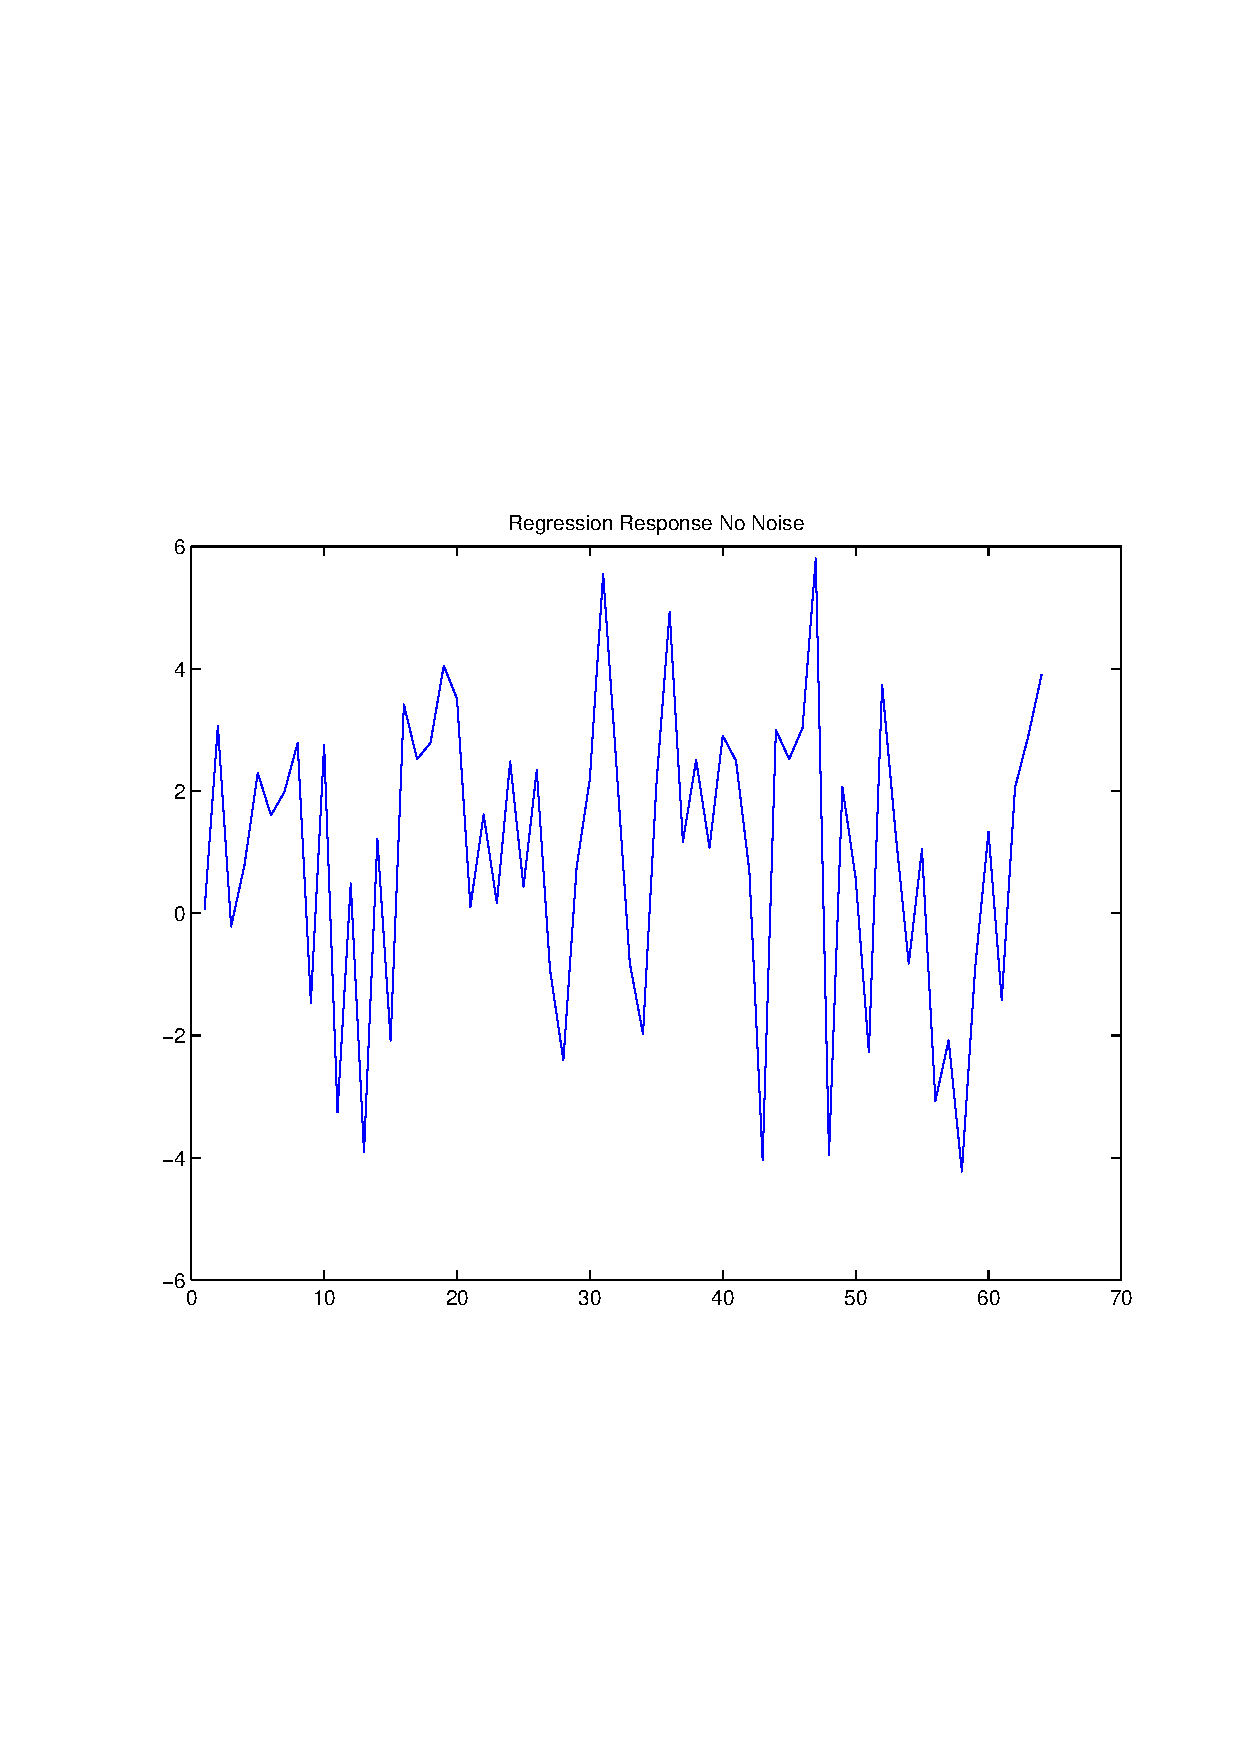
\includegraphics[width=10.0cm,height=10.0cm]{regression_response_no_noise.pdf}

\includegraphics[width=10.0cm,height=10.0cm]{regression_response_with_noise.pdf}

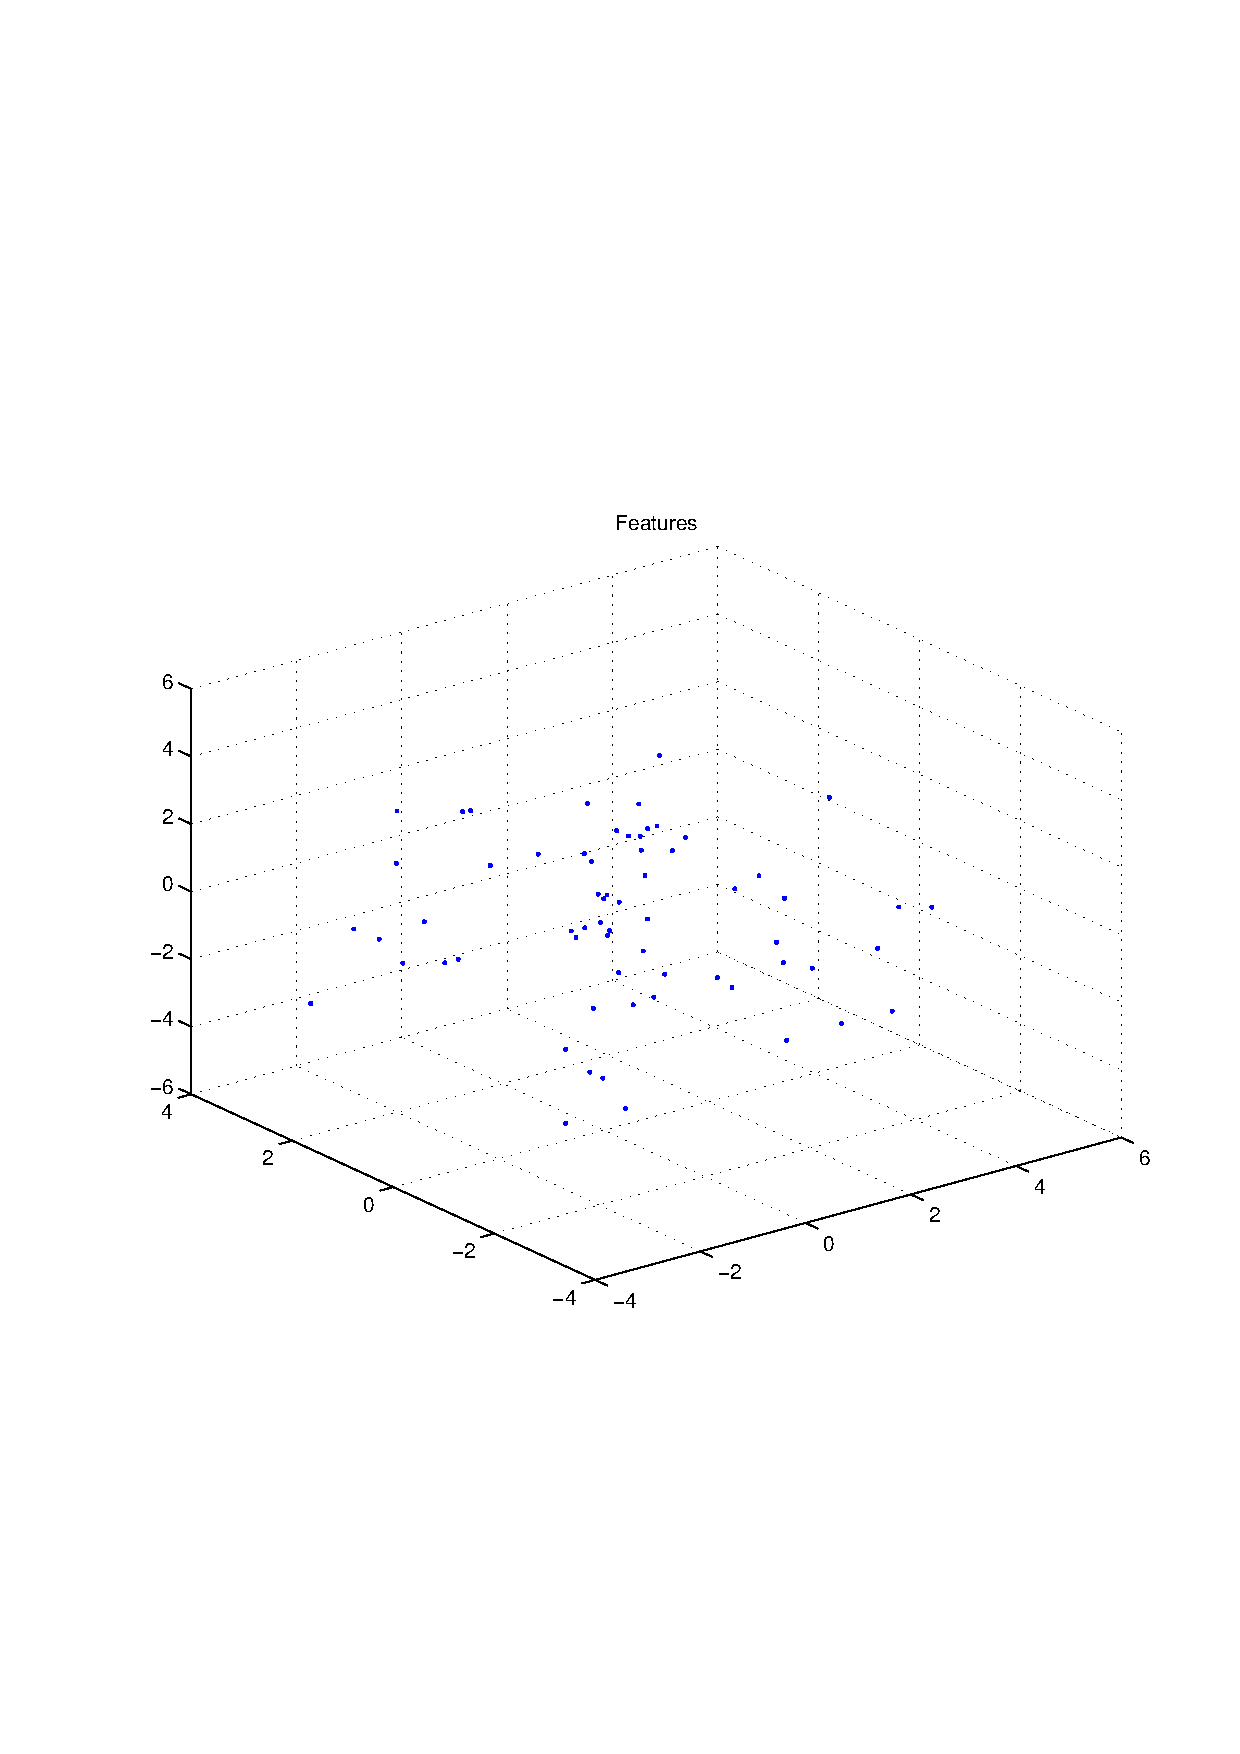
\includegraphics[width=10.0cm,height=10.0cm]{regression_features.pdf}

Beta
+0.817, +0.999, +0.510

Response
-1.988
+1.018
+1.089
+3.215
-0.302
+3.584
+3.527
+0.578
-2.107
+2.014
+2.278
+2.390
+2.607
+3.529
-0.792
+3.011
+0.434
+2.578
+2.879
+4.980
+0.318
-1.611
-3.003
+1.747
-2.648
-0.338
-0.911
-0.057
+2.724
+3.008
+2.694
+3.576
-0.417
+0.086
+0.452
+3.019
+0.269
+0.298
+4.968
+2.699
+1.002
+0.214
+1.035
-1.781
+3.396
+0.348
+1.403
-0.571
+0.770
-0.199
-1.934
-0.054
+2.471
+1.203
+2.724
+0.032
-1.278
+0.944
-0.860
+3.683
+1.061
-1.819
-2.020
-7.039
Estimate for Beta
+0.807
+1.006
+0.503
Error:
-0.011, +0.007, -0.007


QueryPerformanceCounter  =  +3.137
\subsubsection{Fast Gauss Transform}
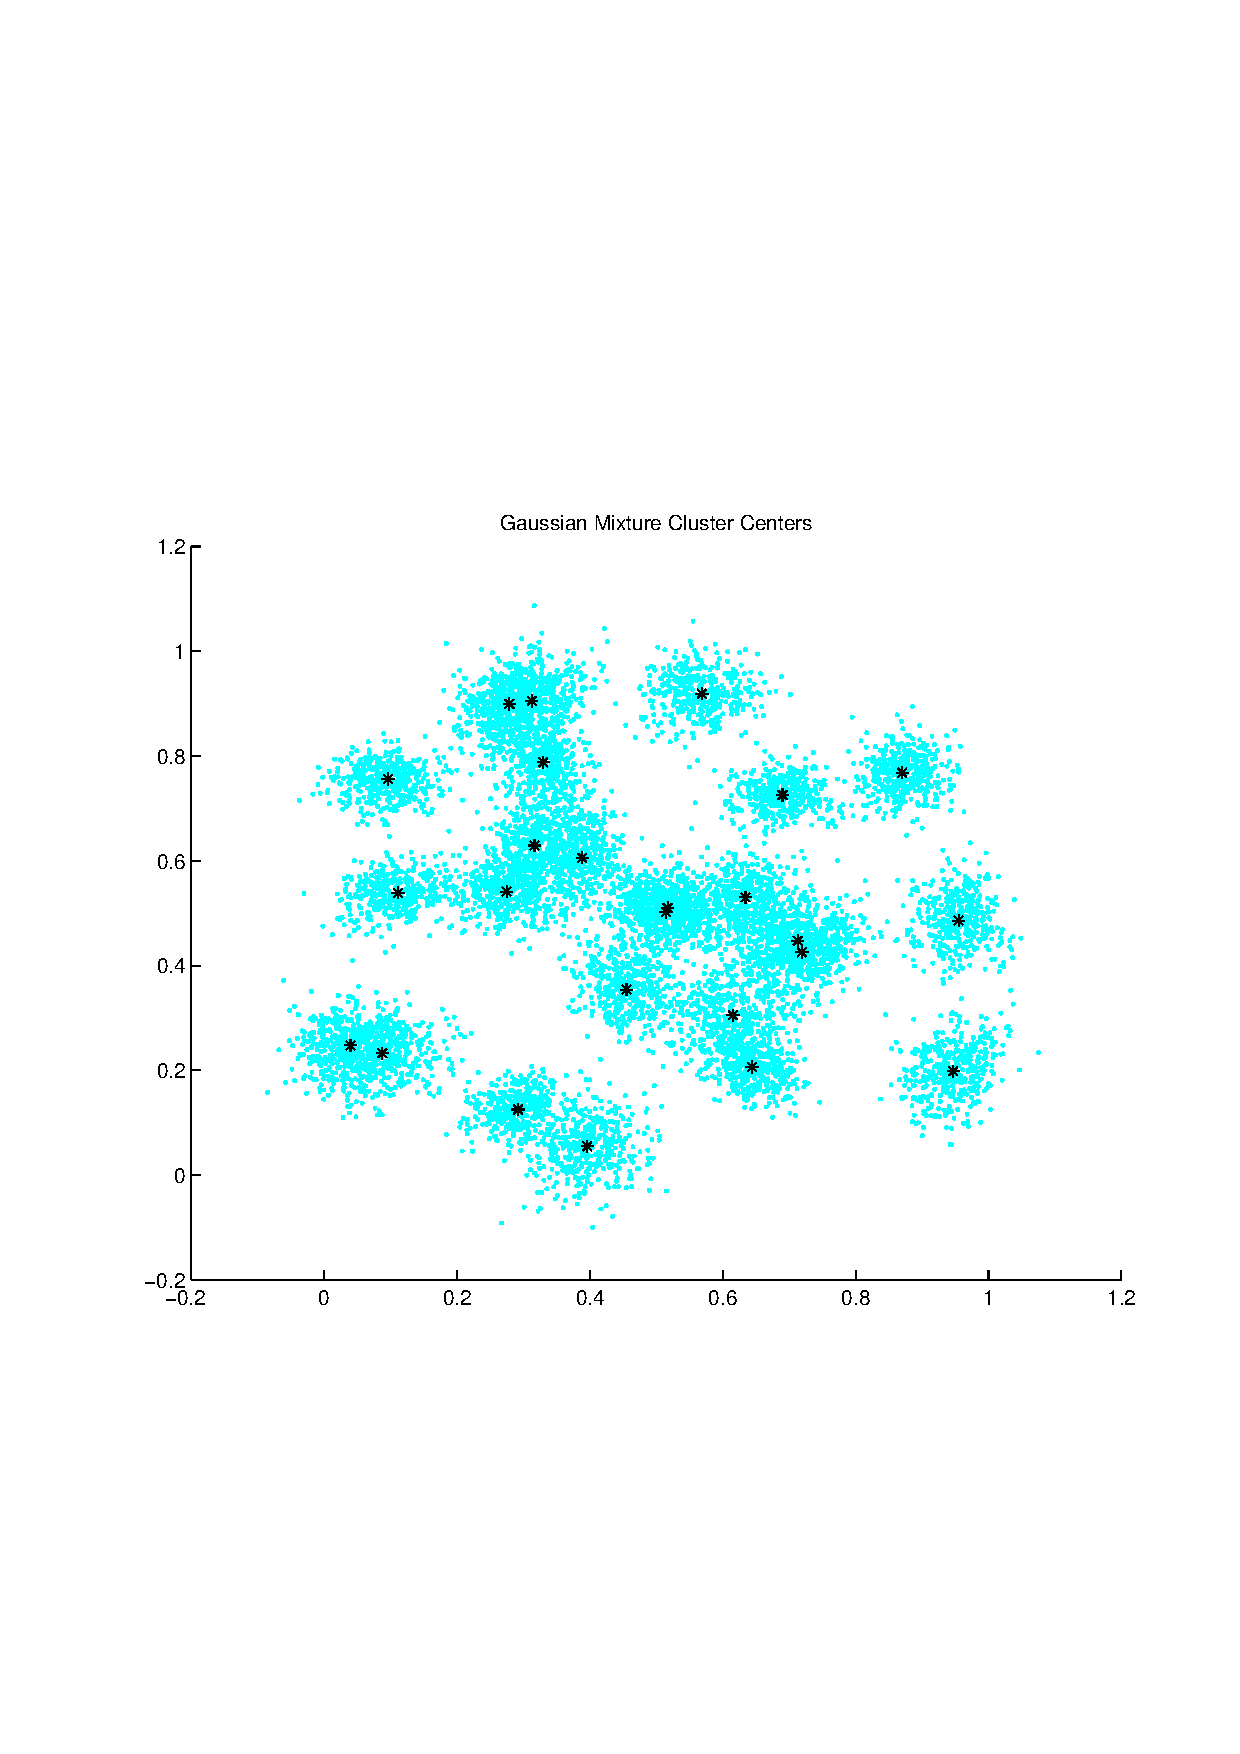
\includegraphics[width=10.0cm,height=10.0cm]{GaussianMixture_ClusterCenters25_Centers.pdf}

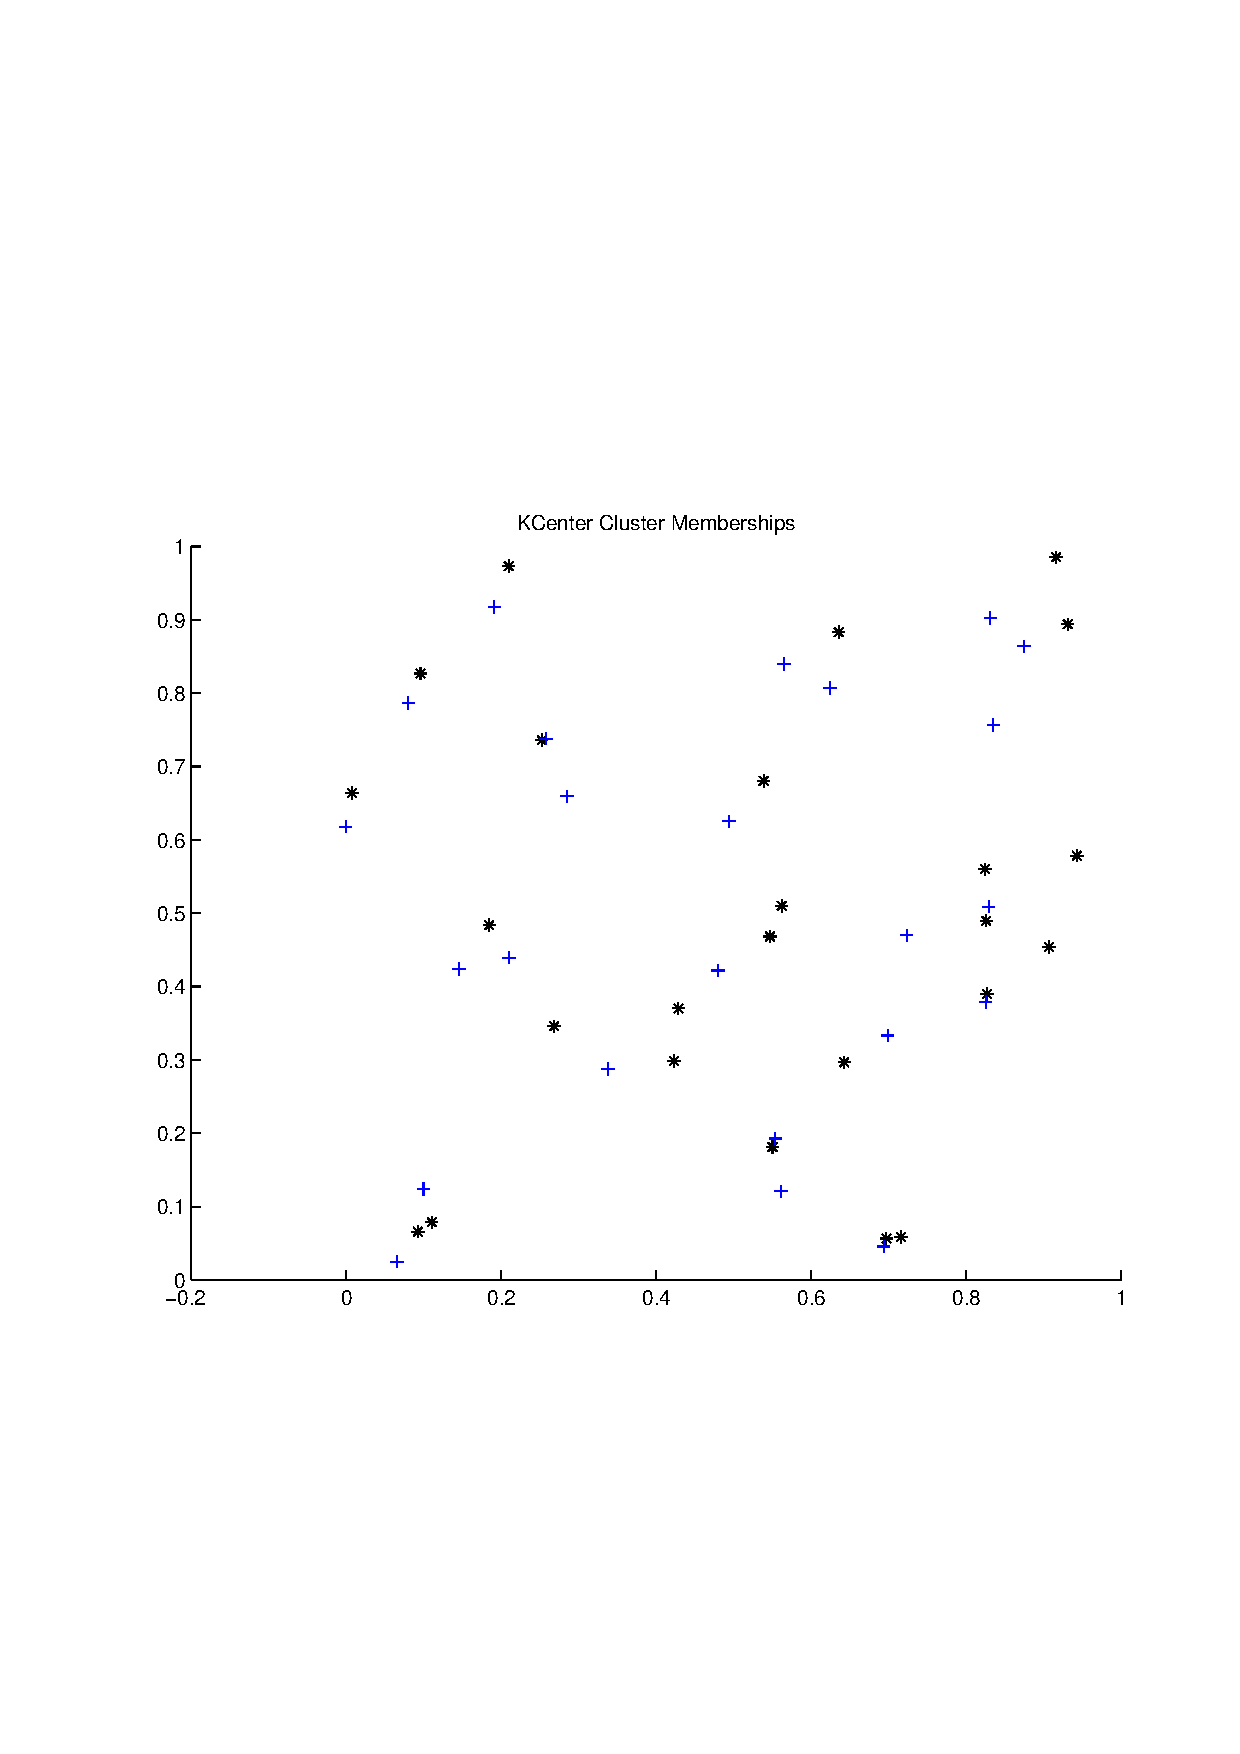
\includegraphics[width=10.0cm,height=10.0cm]{KCenterClusterMemberships_25_Centers.pdf}

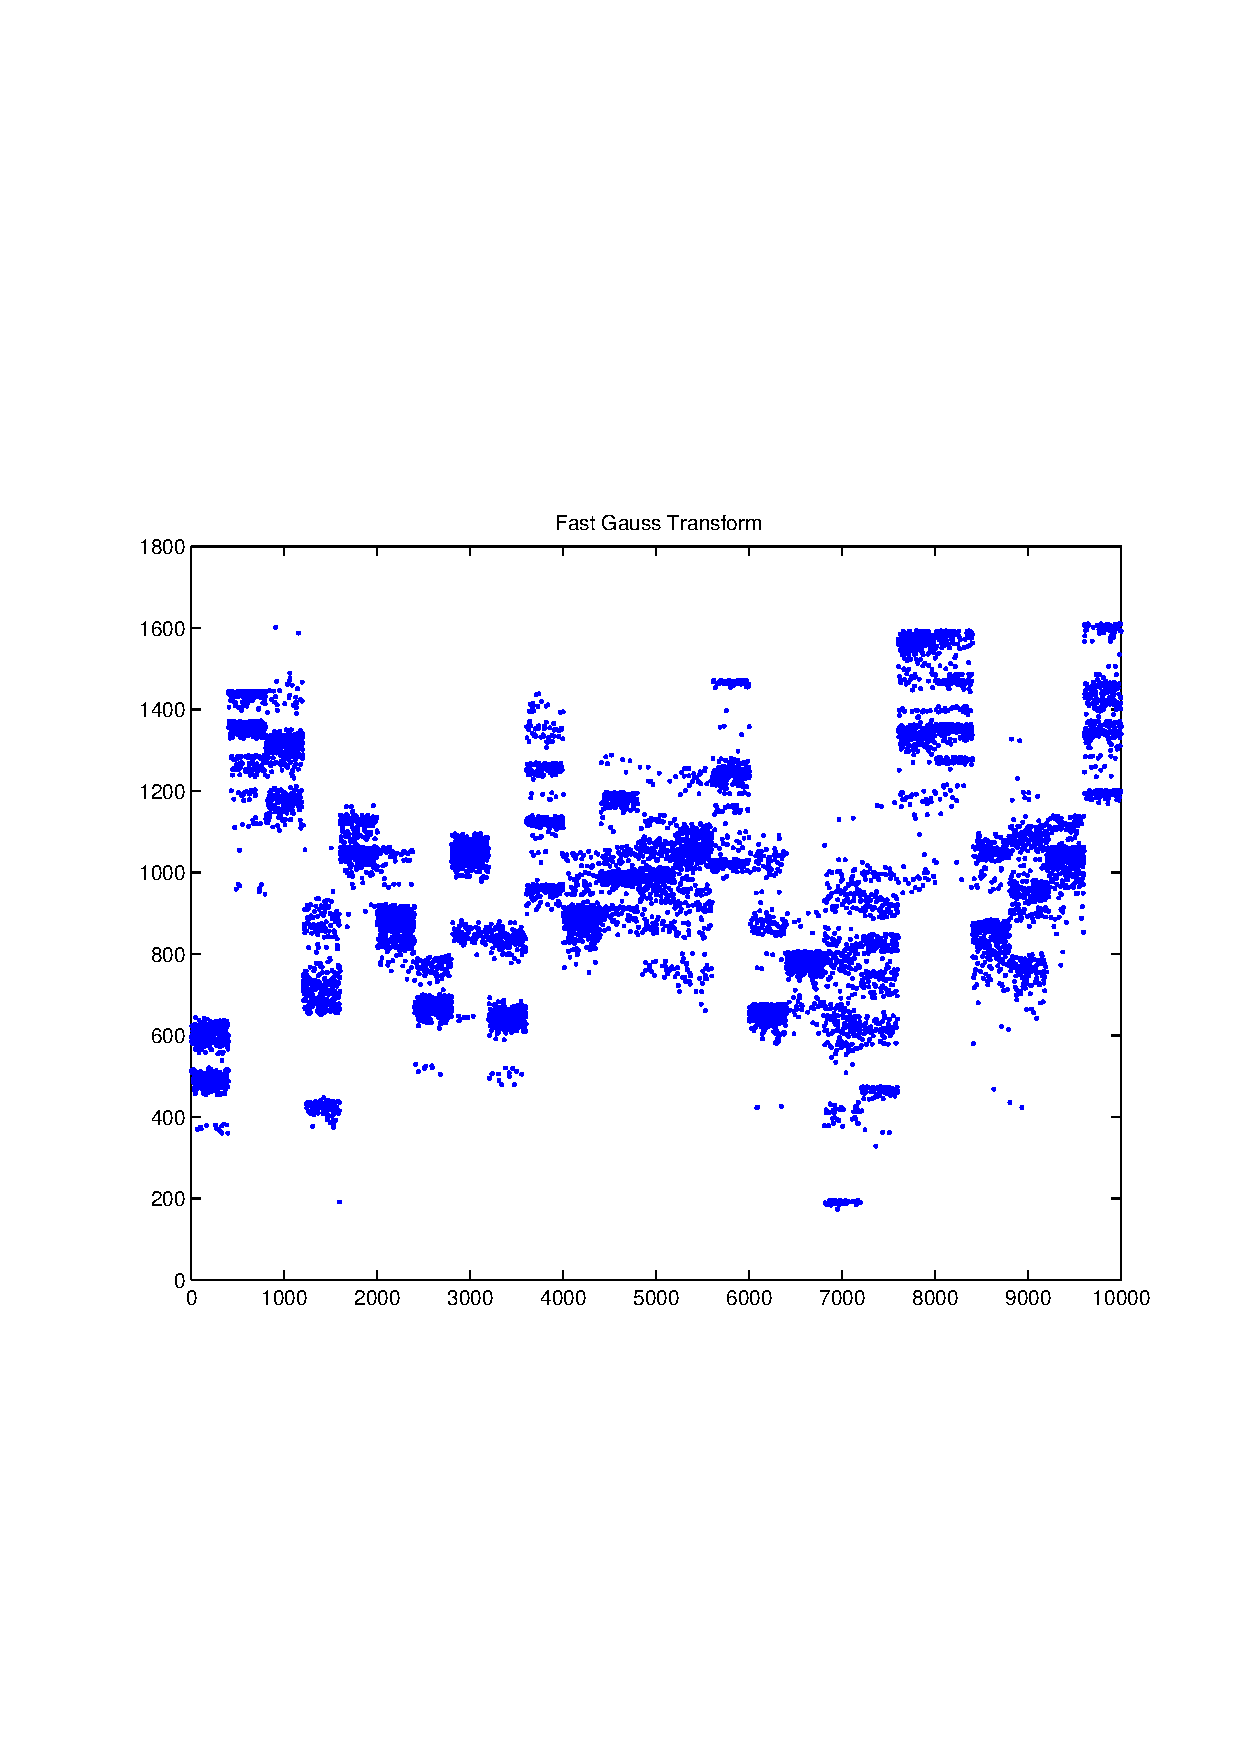
\includegraphics[width=10.0cm,height=10.0cm]{FGT25_Centers.pdf}

QueryPerformanceCounter  =  +7.050
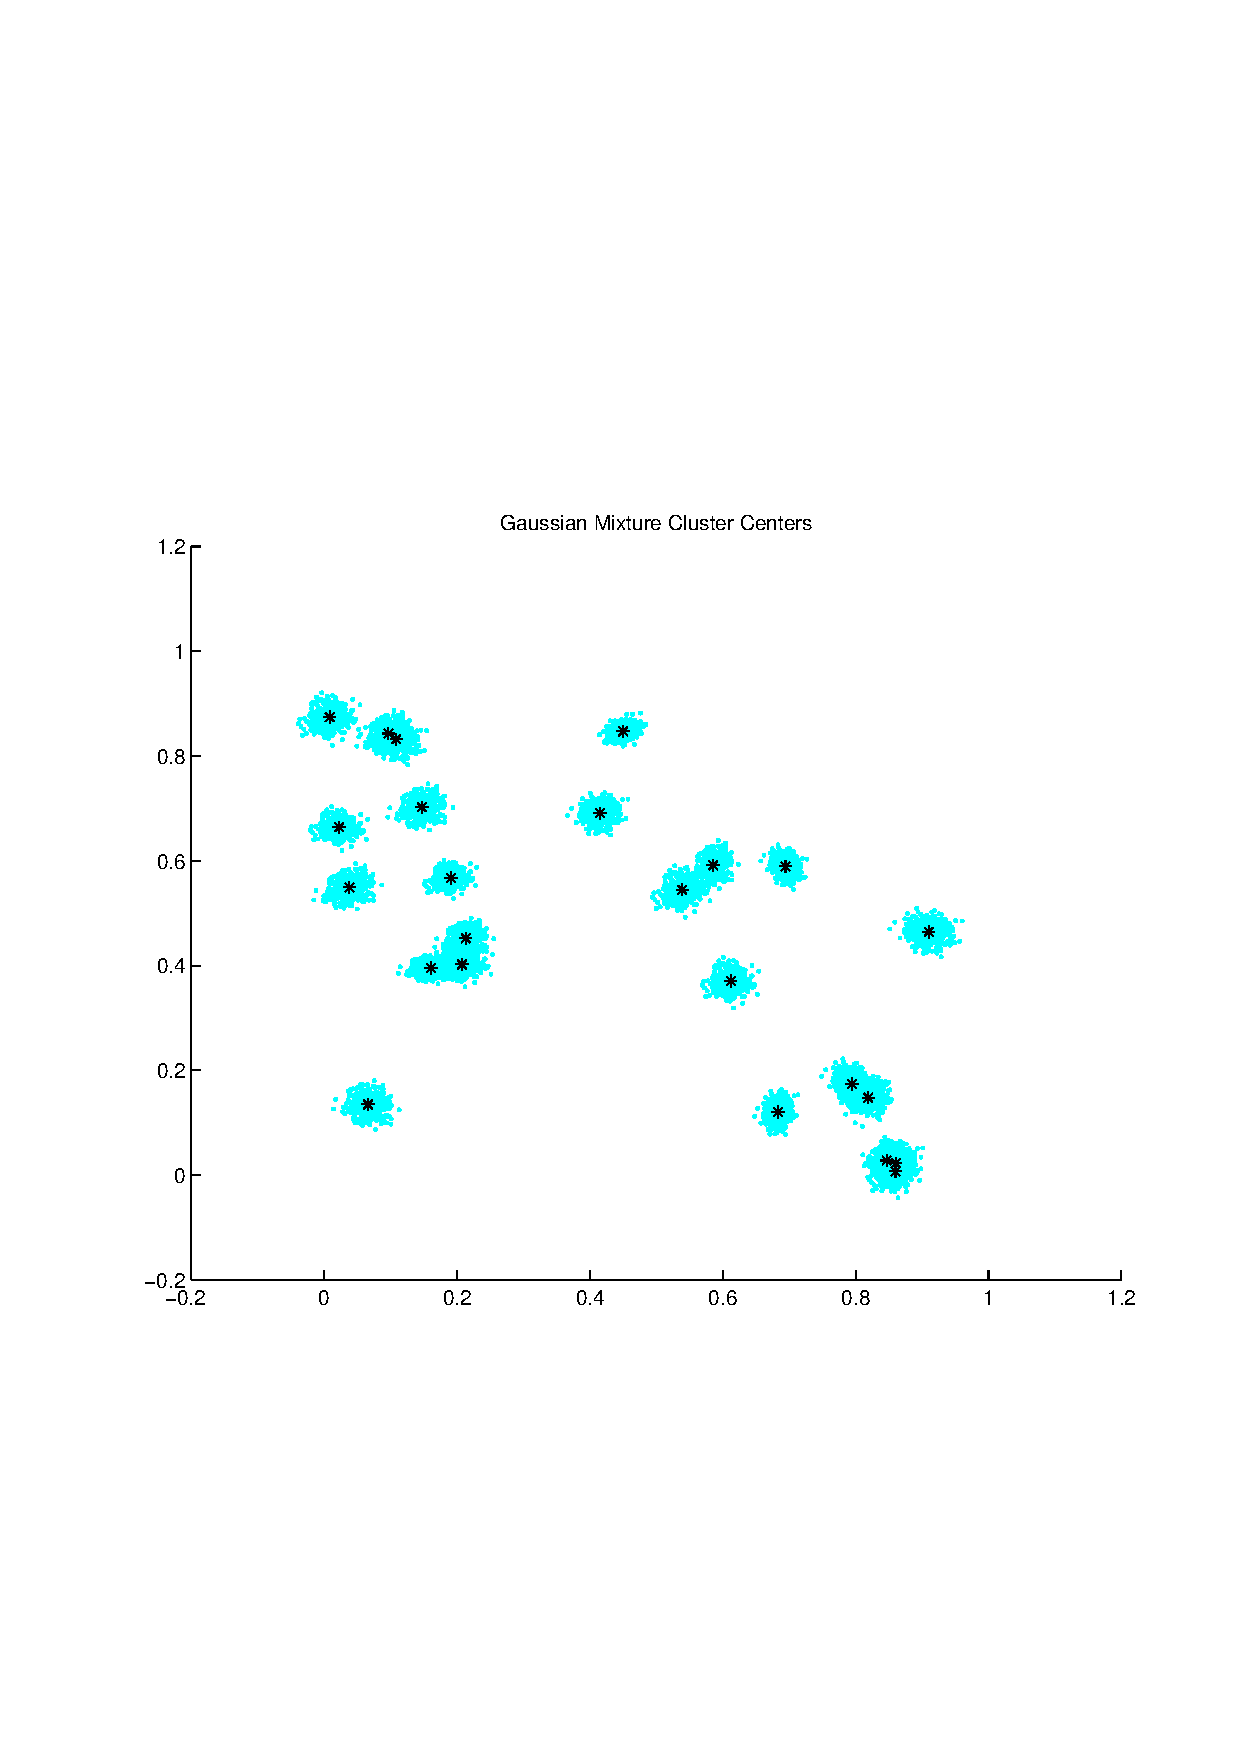
\includegraphics[width=10.0cm,height=10.0cm]{GaussianMixture_ClusterCenters24_Centers.pdf}

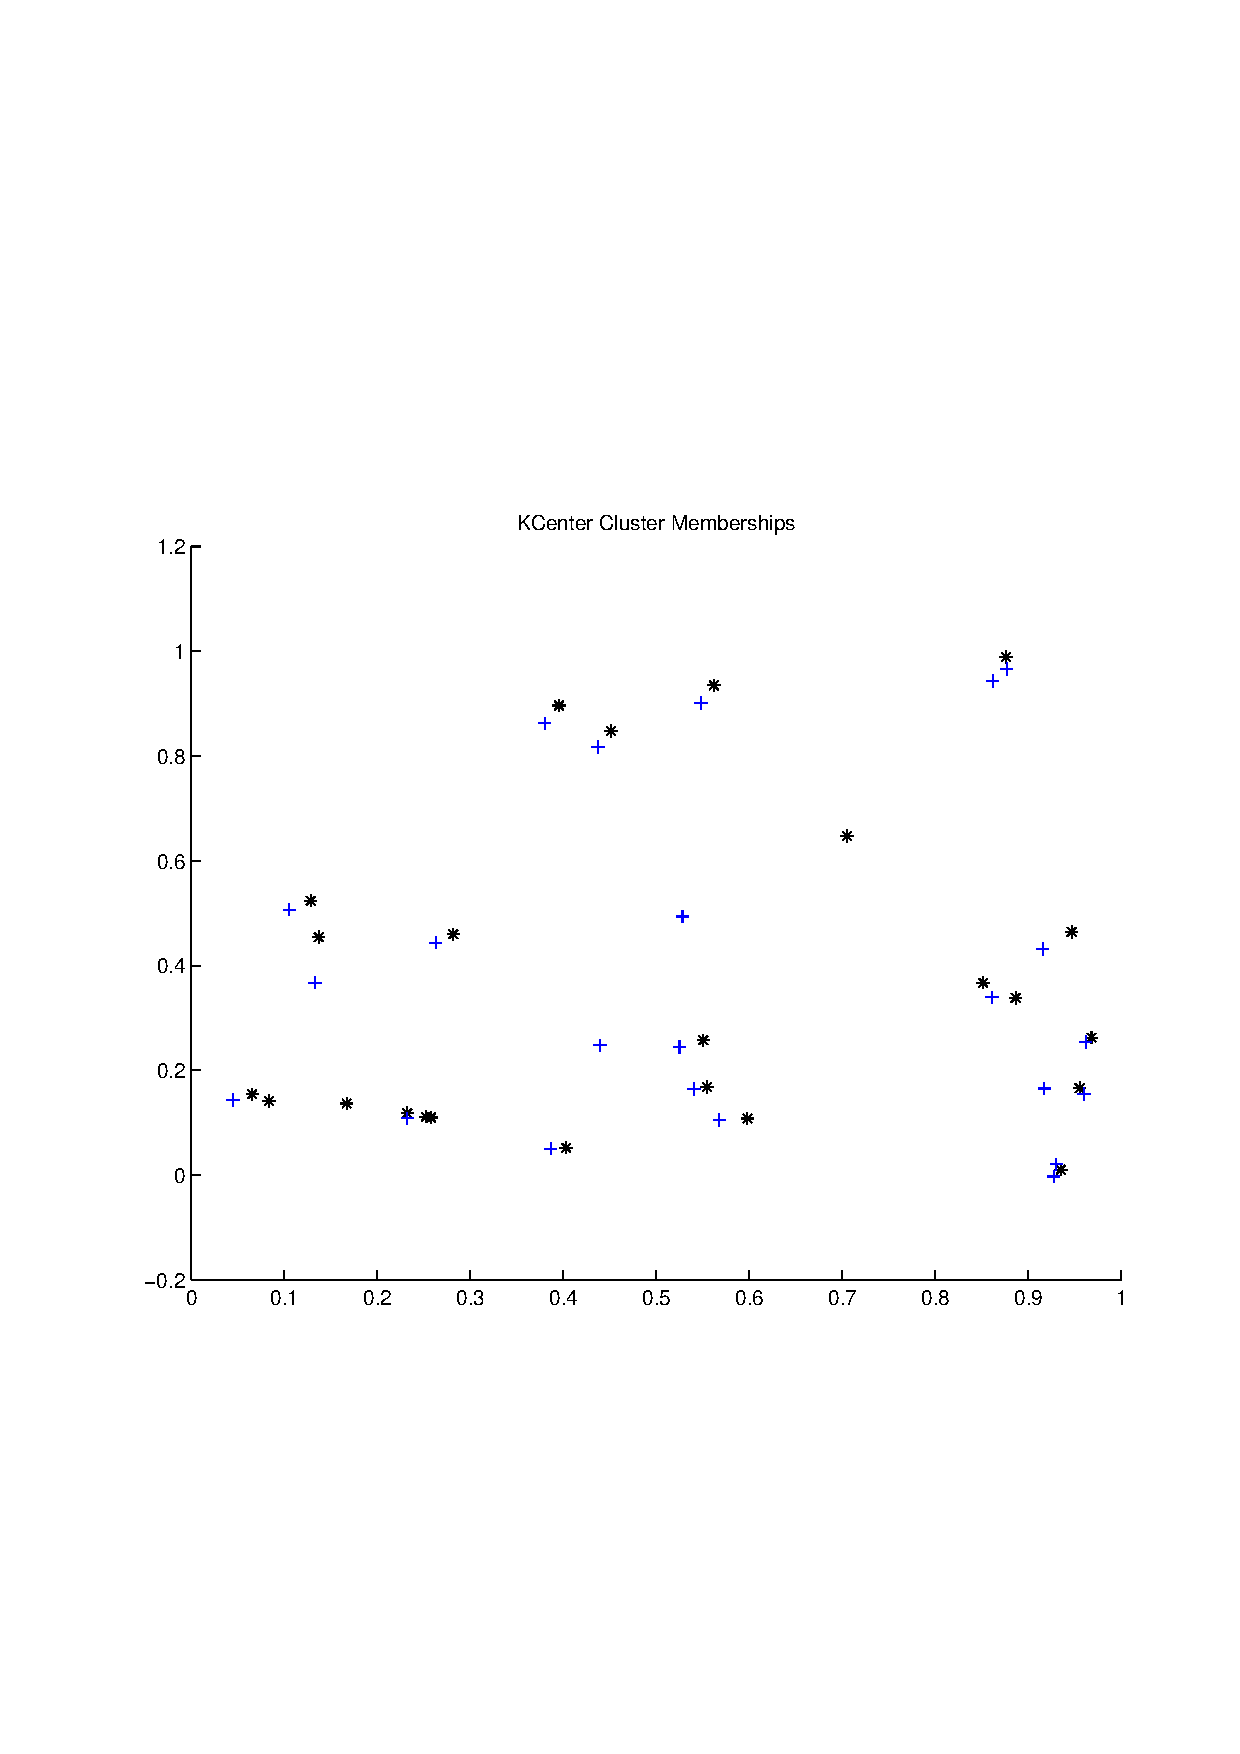
\includegraphics[width=10.0cm,height=10.0cm]{KCenterClusterMemberships_24_Centers.pdf}

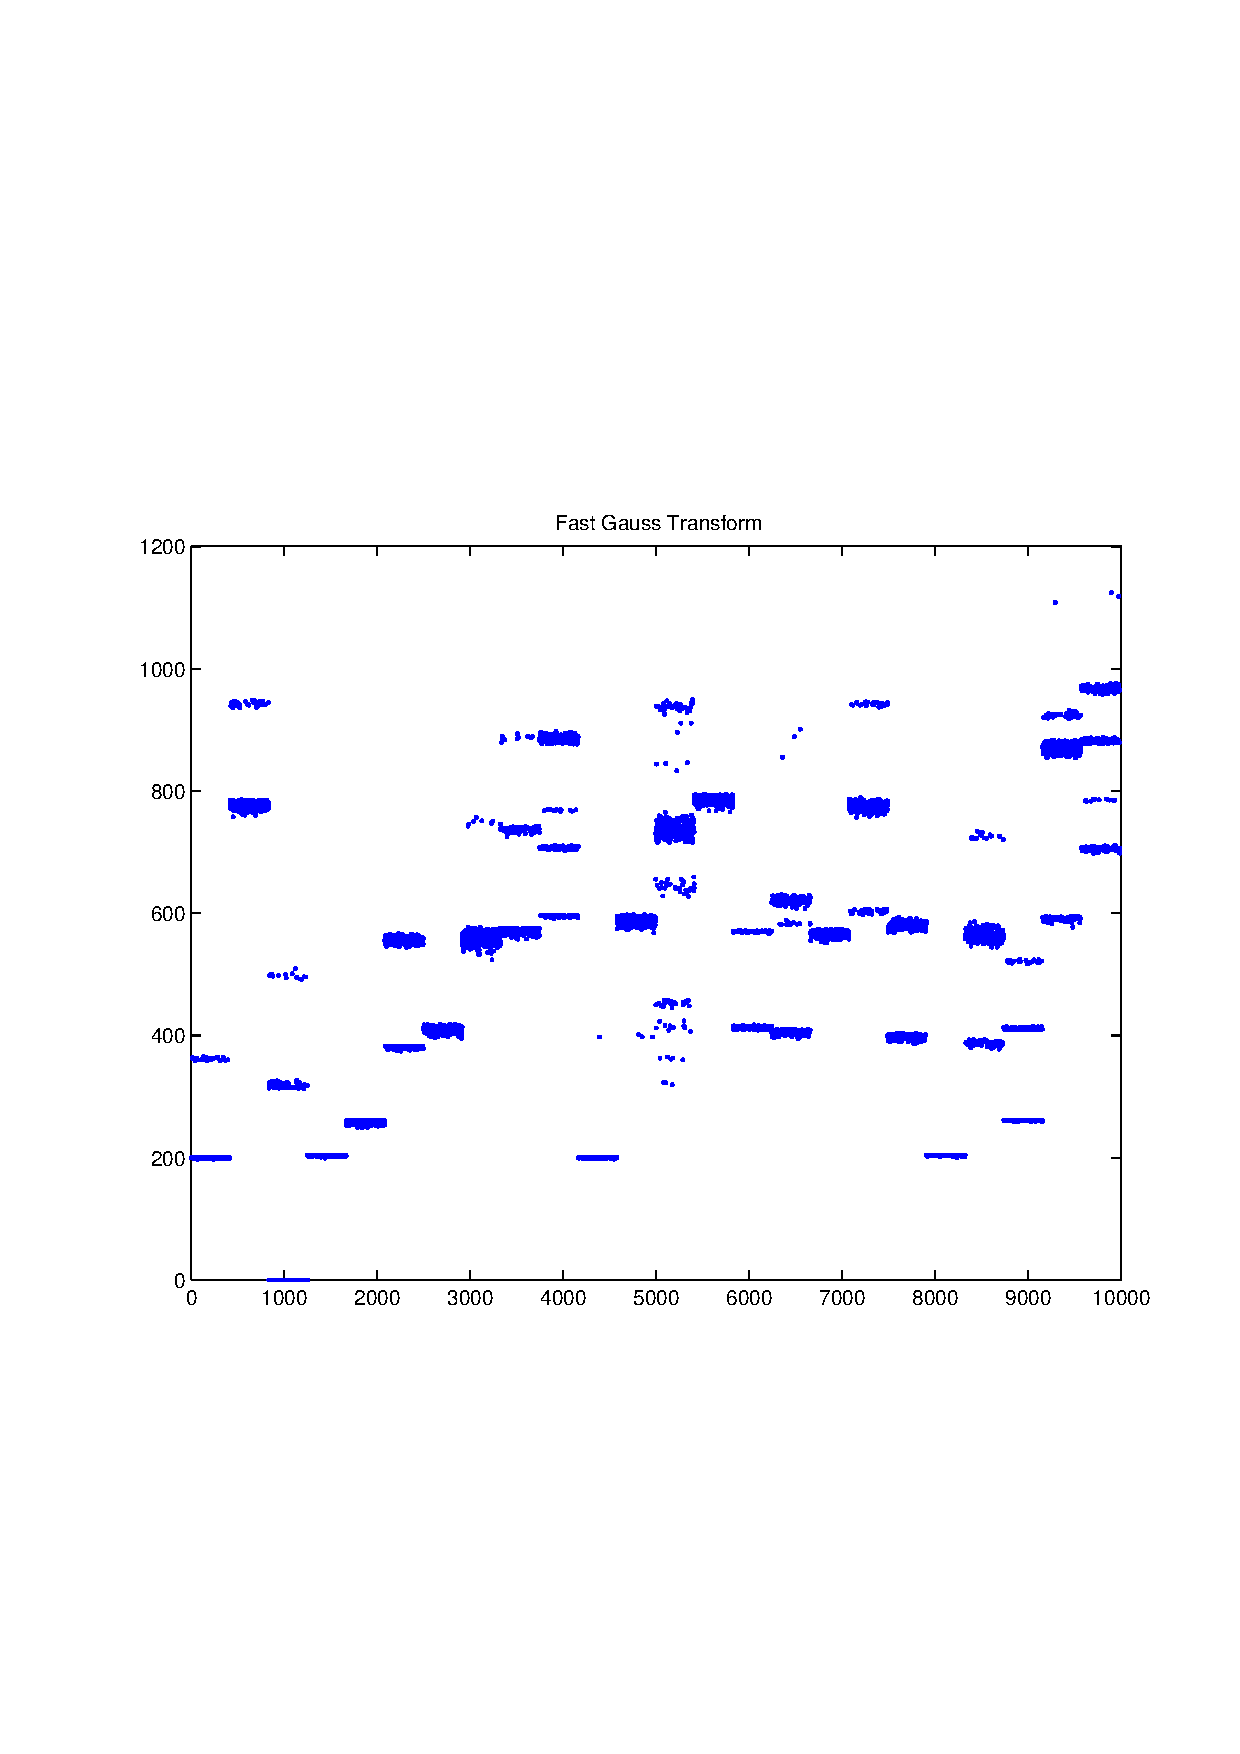
\includegraphics[width=10.0cm,height=10.0cm]{FGT24_Centers.pdf}

QueryPerformanceCounter  =  +6.948
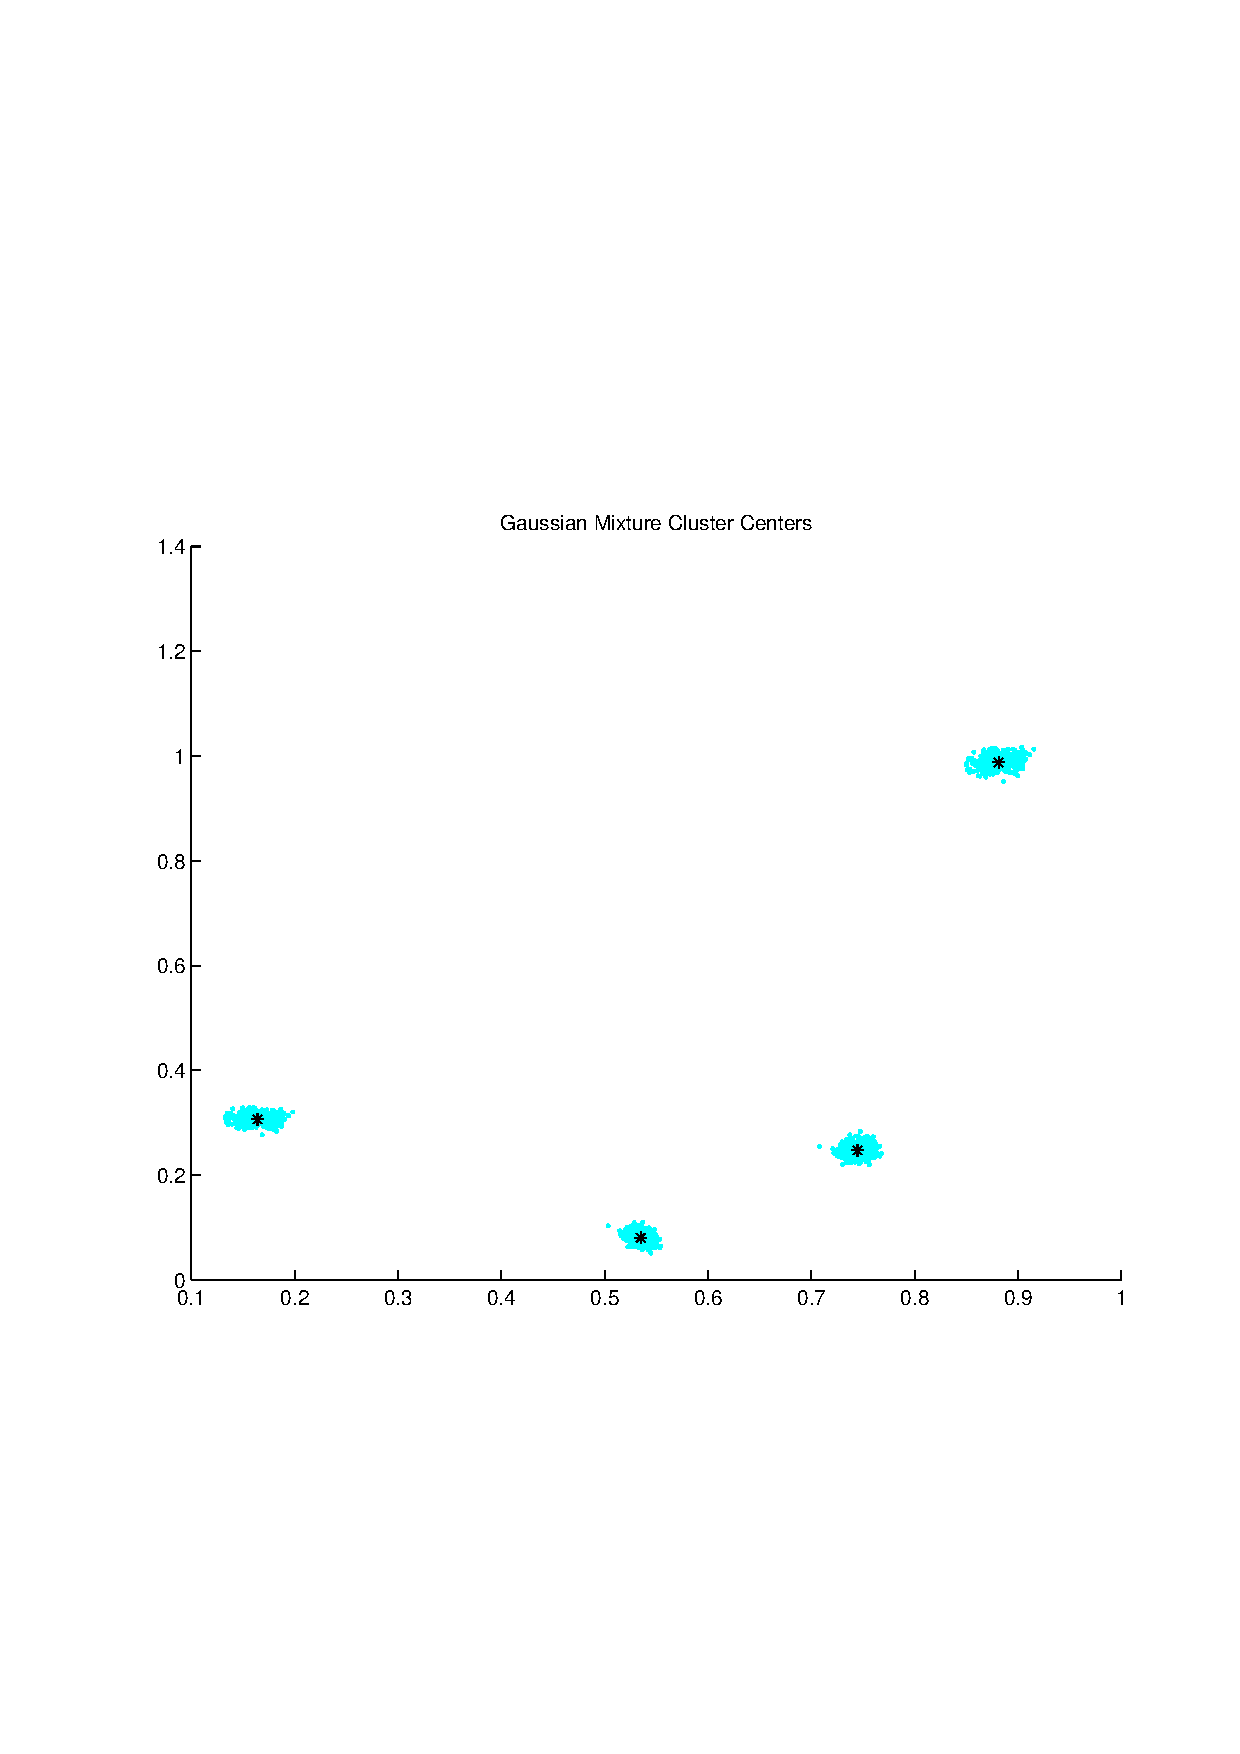
\includegraphics[width=10.0cm,height=10.0cm]{GaussianMixture_ClusterCenters4_Centers.pdf}

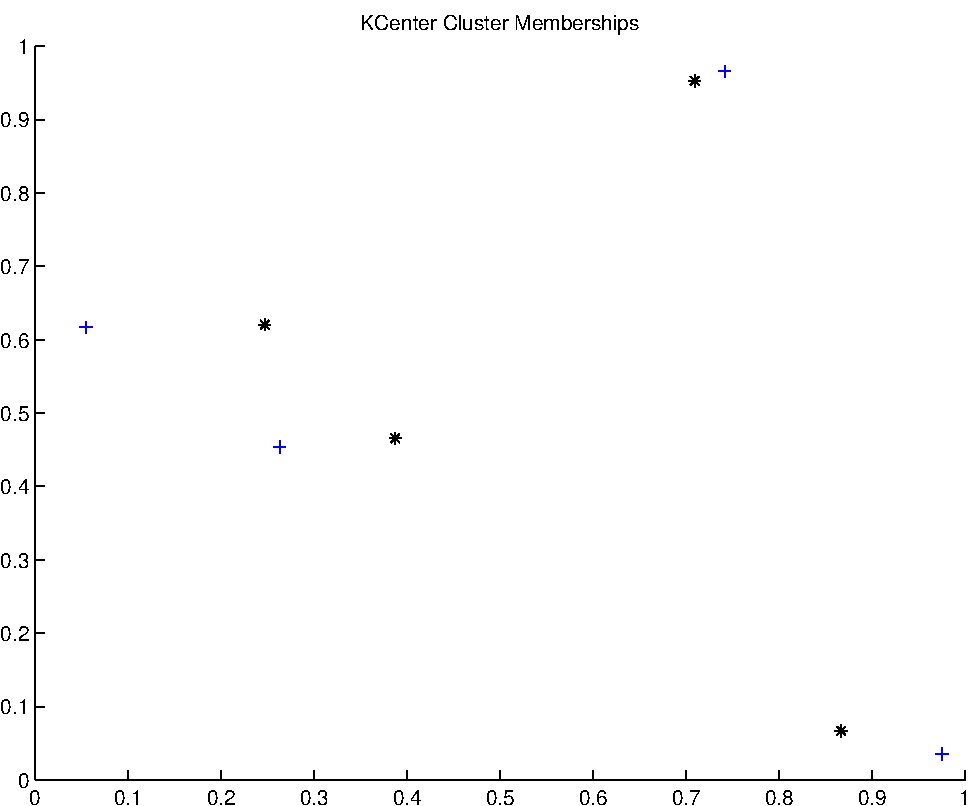
\includegraphics[width=10.0cm,height=10.0cm]{KCenterClusterMemberships_4_Centers.pdf}

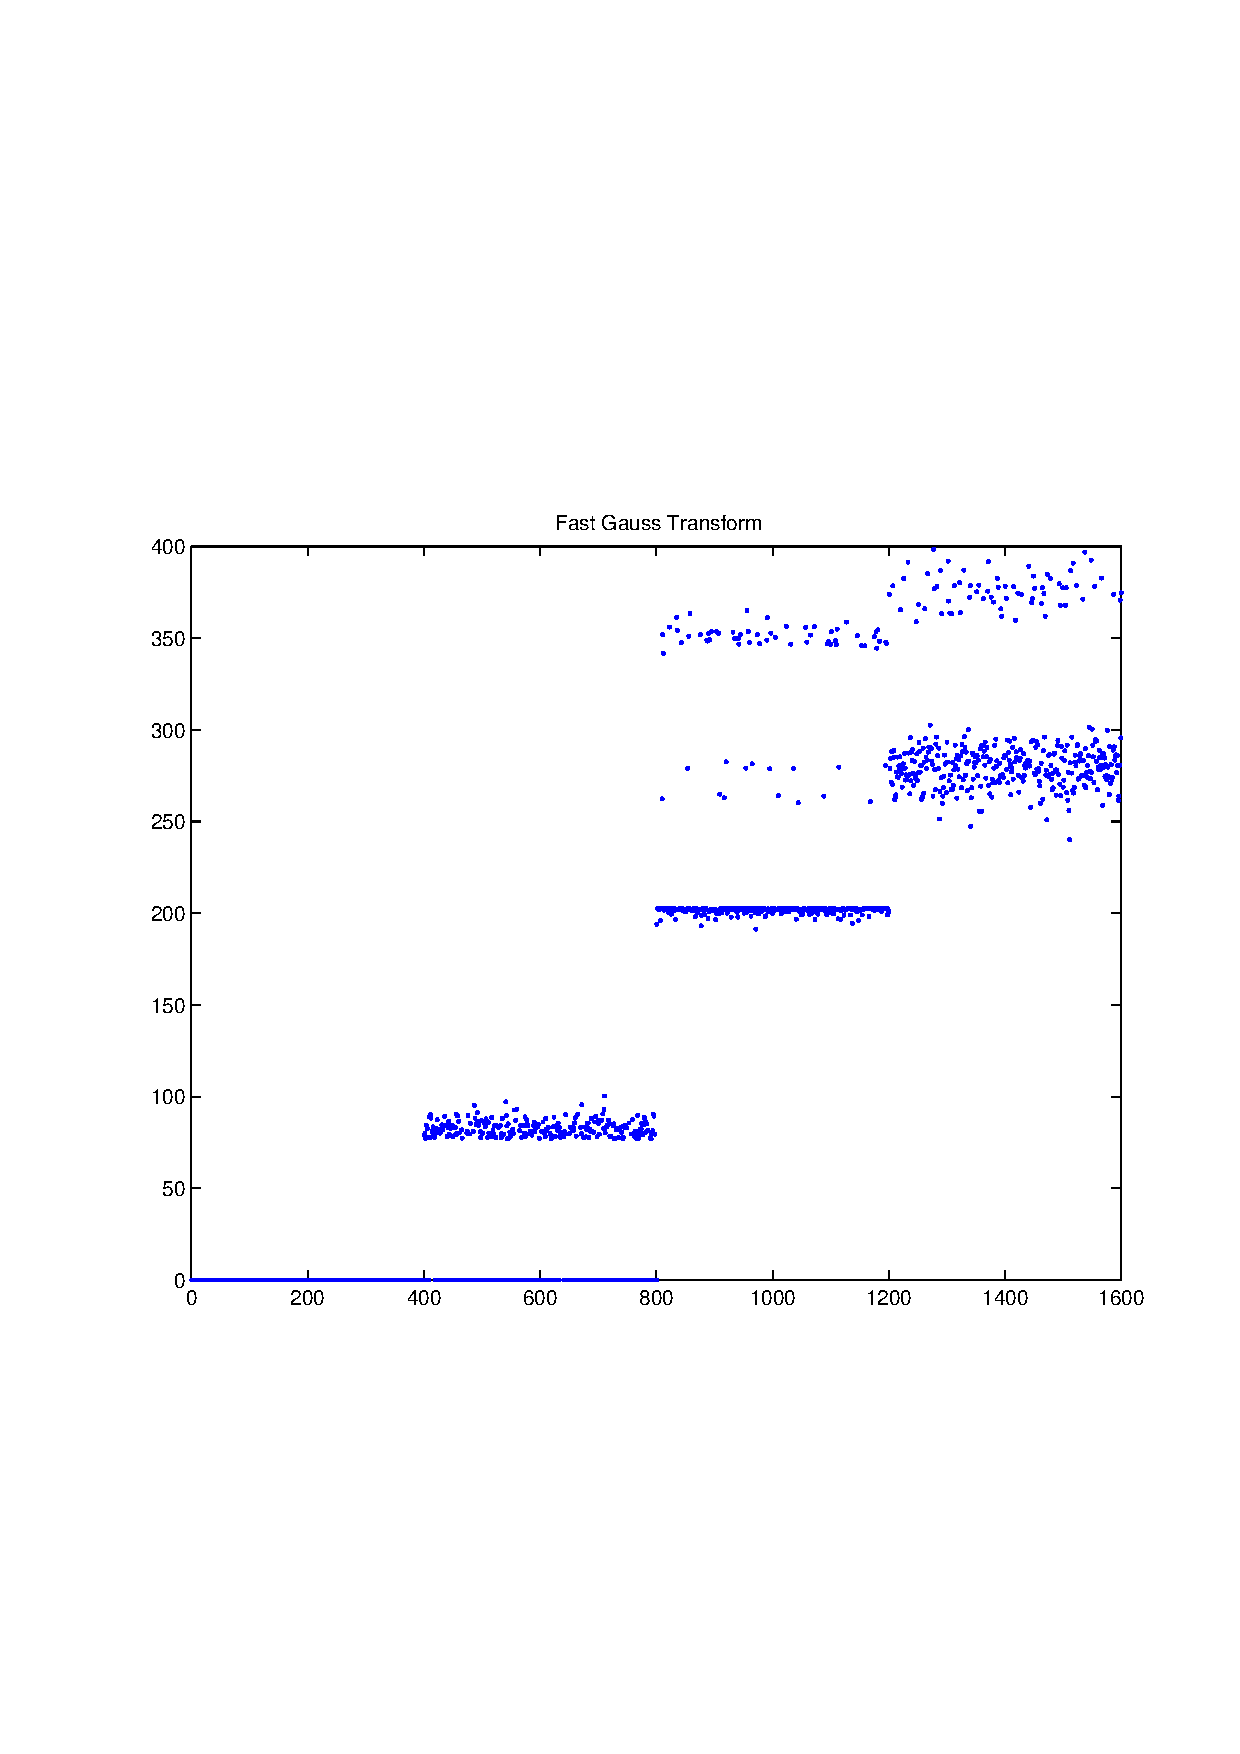
\includegraphics[width=10.0cm,height=10.0cm]{FGT4_Centers.pdf}

QueryPerformanceCounter  =  +3.969
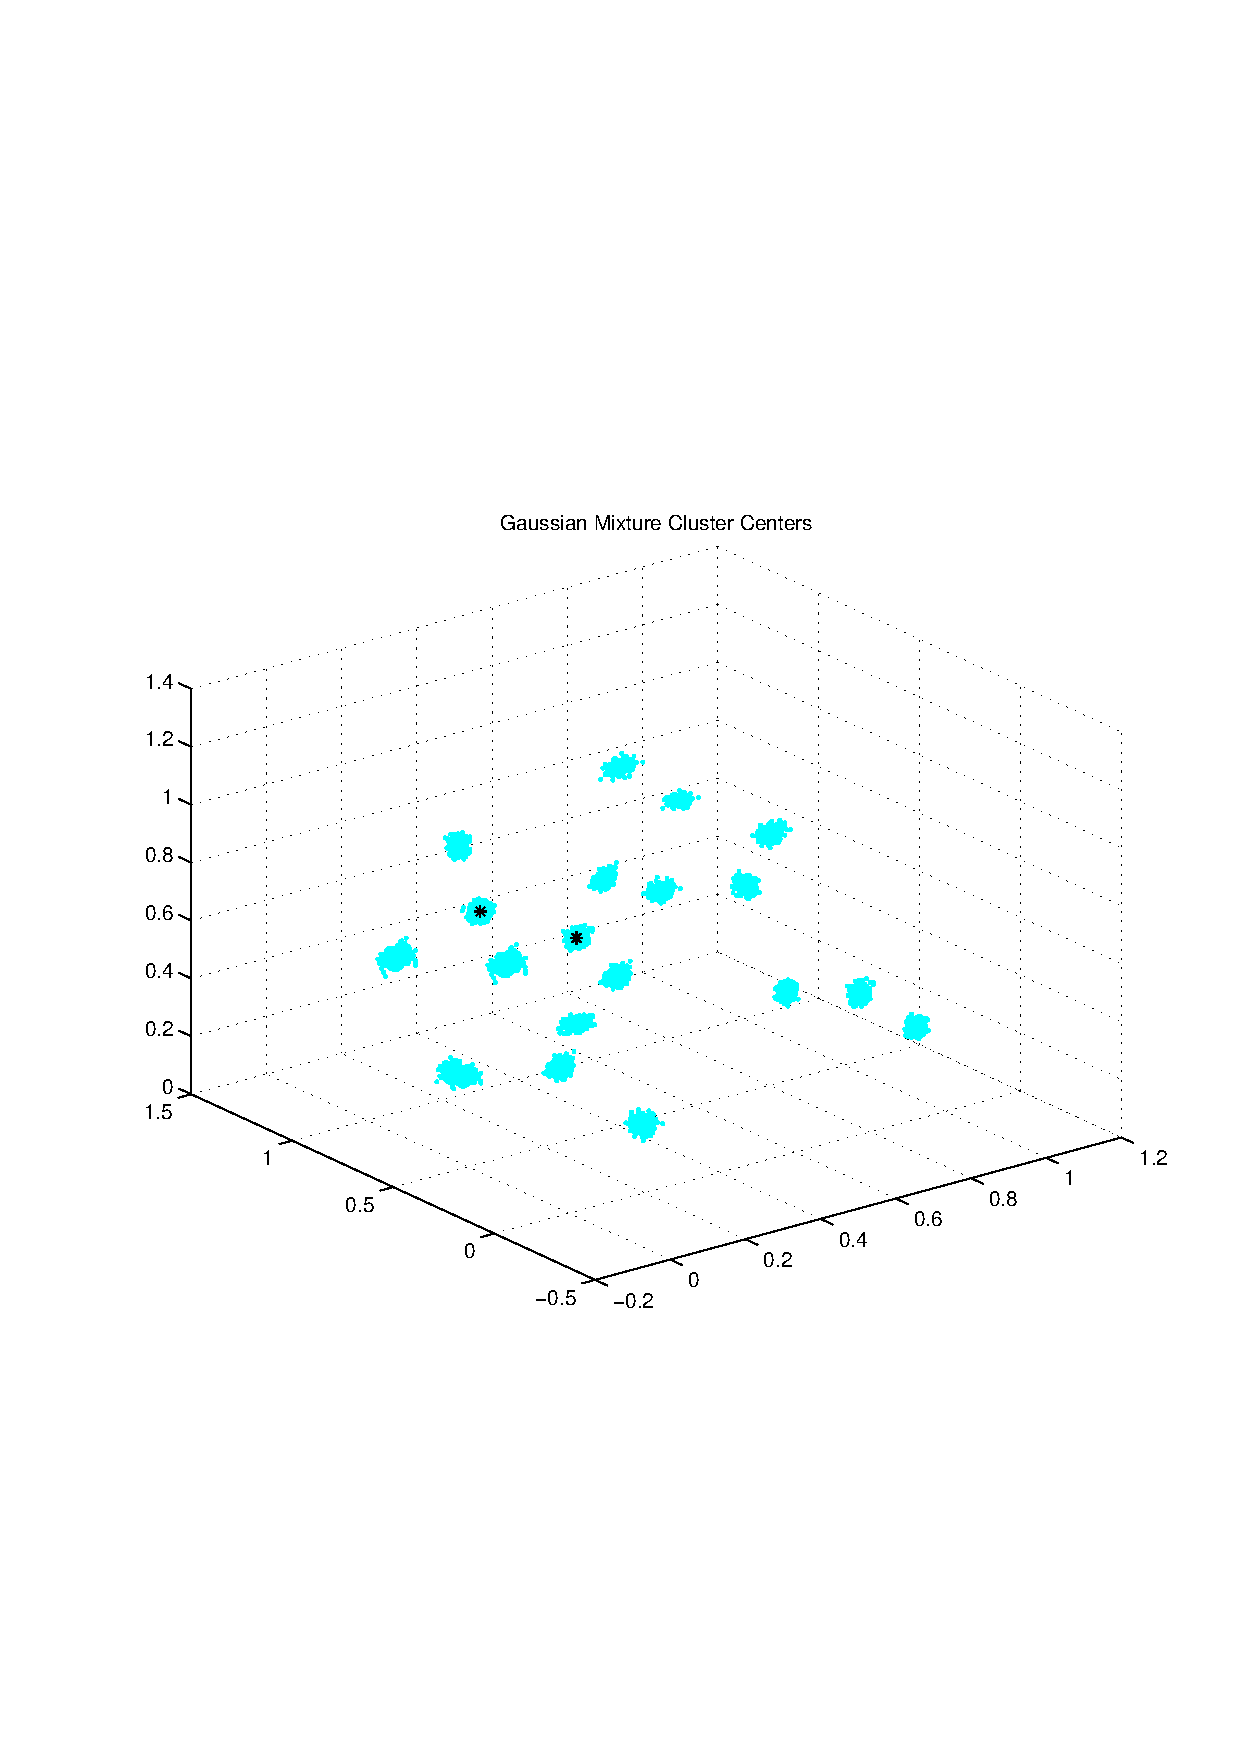
\includegraphics[width=10.0cm,height=10.0cm]{GaussianMixture_ClusterCenters20_Centers.pdf}

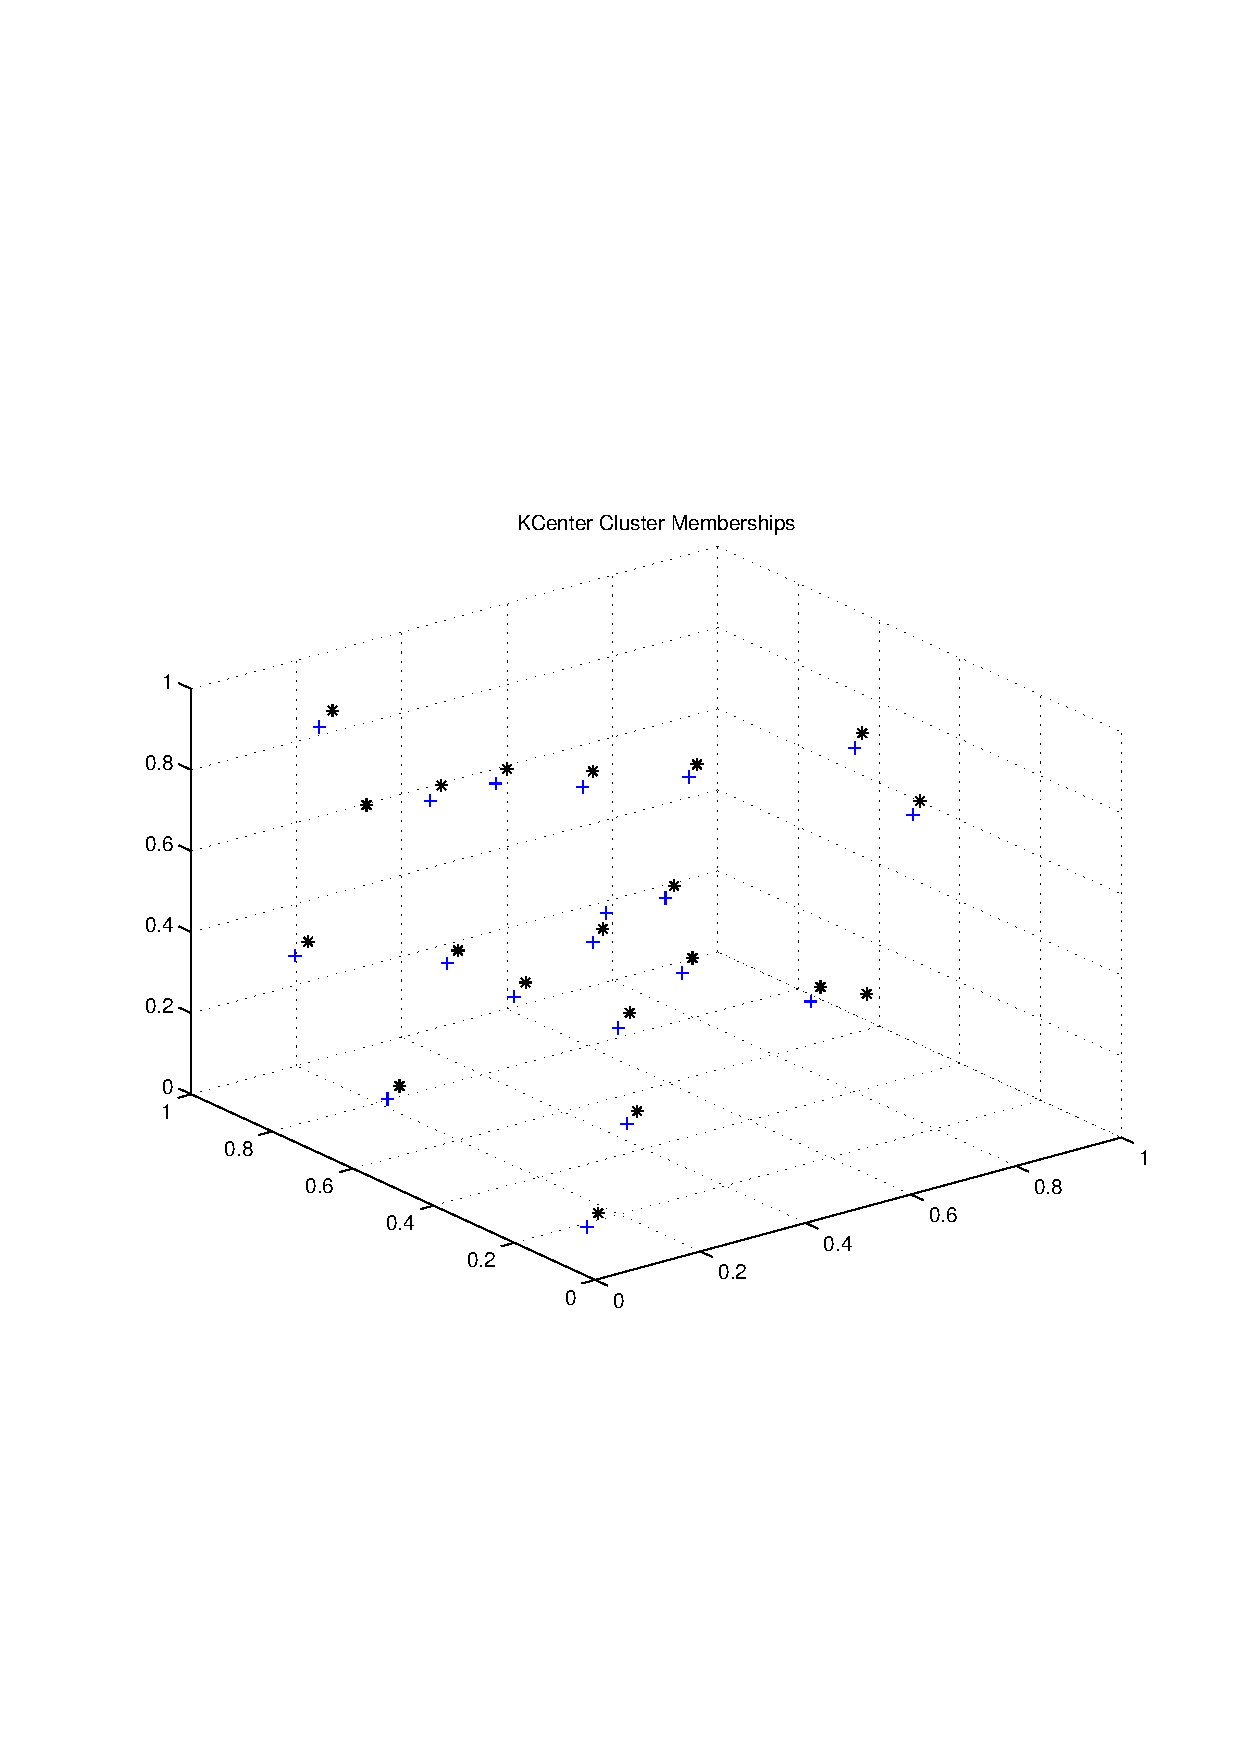
\includegraphics[width=10.0cm,height=10.0cm]{KCenterClusterMemberships_20_Centers.pdf}

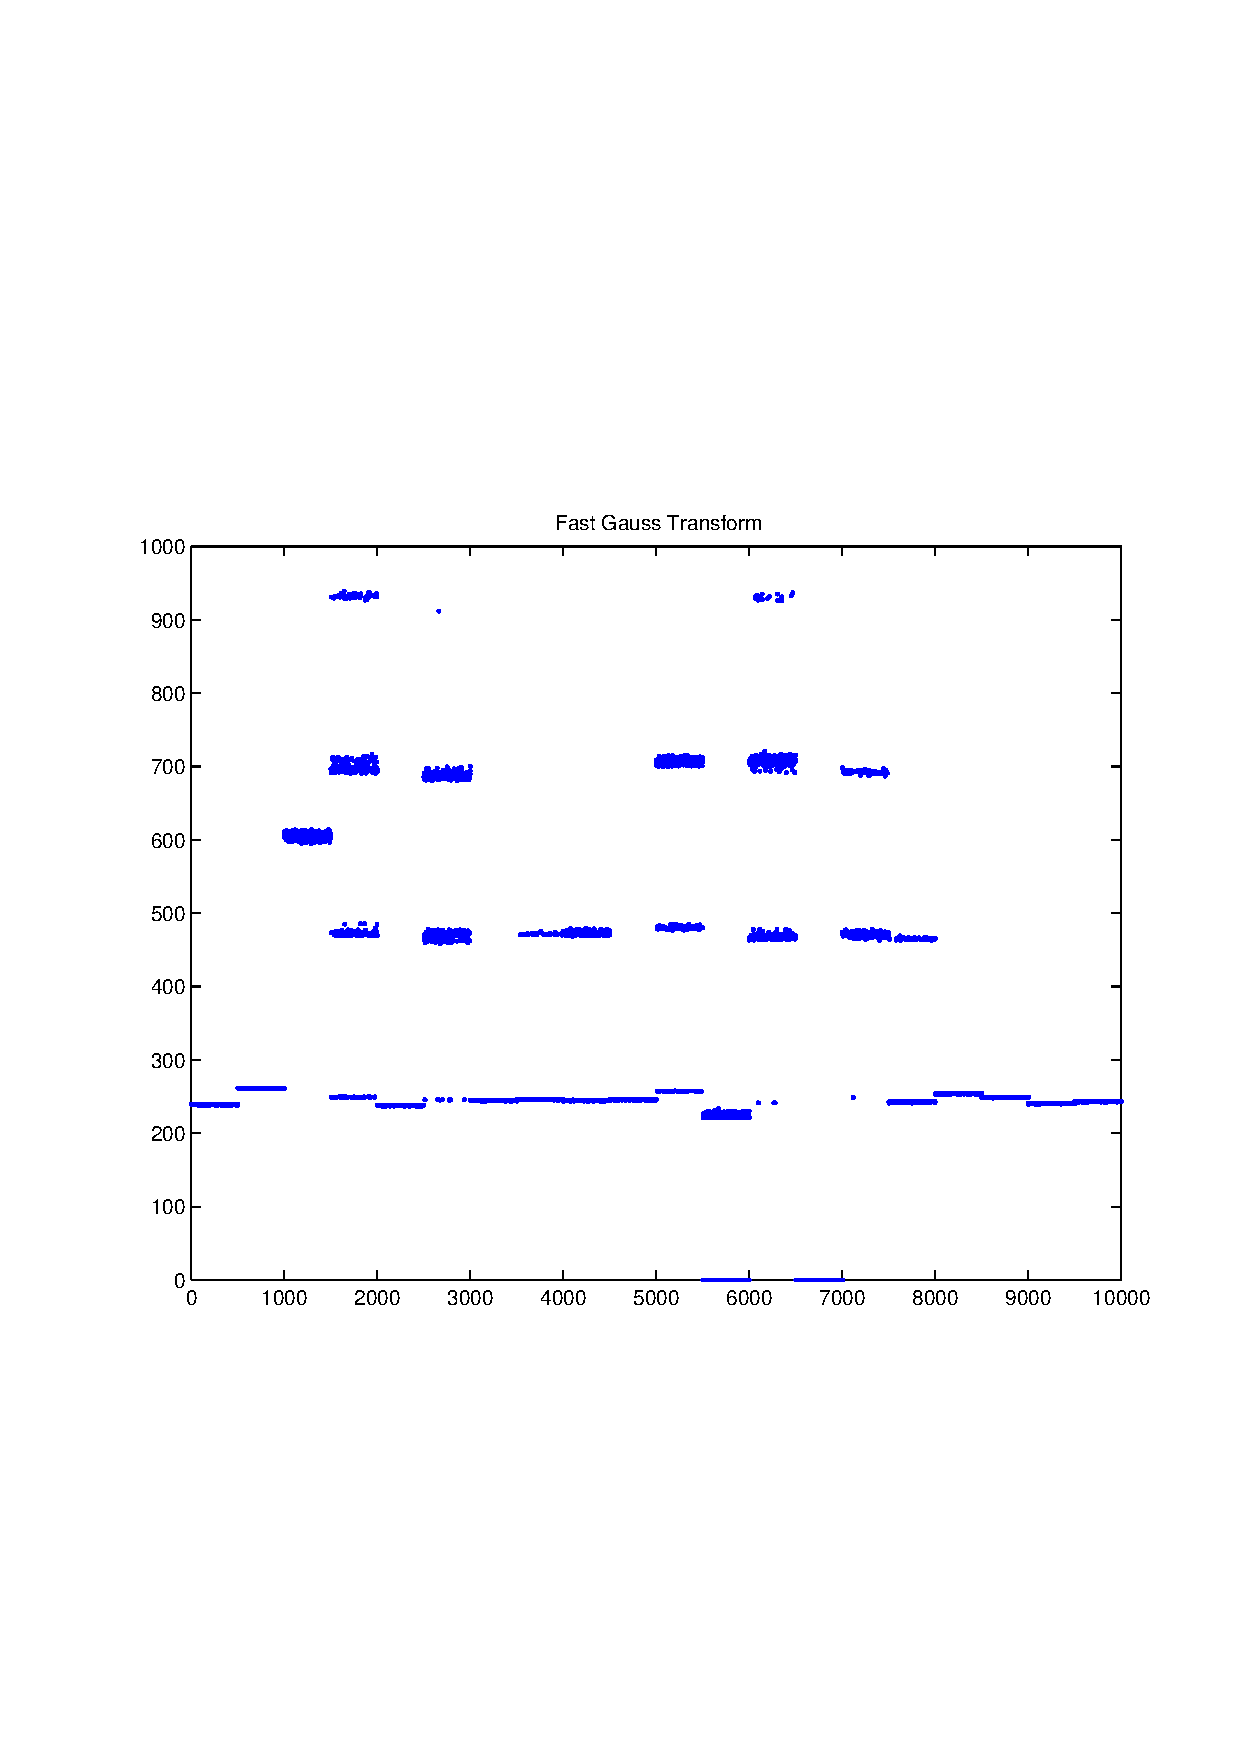
\includegraphics[width=10.0cm,height=10.0cm]{FGT20_Centers.pdf}

QueryPerformanceCounter  =  +6.243
\subsubsection{Matrix Norms}
\subsubsection{Haar Distributed Random Orthogonal Matrix $A \in O(n)$}
 Testing Operator Norm
Number of Dimensions: +12

$A = \left(
\begin{array}{
cccccccccccc}
+0.171 & -0.369 & -0.518 & +0.058 & +0.056 & +0.485 & +0.096 & +0.446 & -0.083 & +0.077 & -0.119 & +0.299 \\
+0.237 & -0.283 & +0.173 & -0.335 & +0.484 & -0.415 & +0.108 & +0.079 & +0.255 & -0.239 & -0.095 & +0.407 \\
-0.041 & +0.340 & -0.053 & -0.032 & +0.100 & +0.424 & -0.495 & -0.336 & +0.272 & -0.253 & -0.038 & +0.438 \\
+0.469 & -0.421 & +0.300 & -0.203 & -0.328 & +0.245 & -0.049 & -0.430 & -0.248 & -0.053 & -0.222 & -0.051 \\
+0.018 & -0.192 & -0.434 & +0.021 & +0.140 & -0.319 & -0.569 & -0.082 & +0.027 & +0.015 & -0.426 & -0.374 \\
+0.122 & -0.015 & +0.130 & -0.273 & +0.194 & +0.279 & -0.217 & +0.352 & -0.031 & -0.479 & +0.361 & -0.496 \\
+0.351 & +0.148 & -0.042 & -0.272 & +0.184 & +0.185 & +0.064 & -0.086 & +0.484 & +0.625 & +0.104 & -0.251 \\
+0.258 & -0.193 & +0.059 & +0.436 & +0.286 & -0.117 & -0.333 & -0.123 & -0.276 & +0.241 & +0.570 & +0.149 \\
-0.177 & -0.478 & -0.054 & +0.116 & -0.455 & -0.080 & -0.090 & -0.020 & +0.616 & -0.108 & +0.333 & +0.004 \\
-0.096 & -0.153 & +0.539 & +0.522 & +0.249 & +0.244 & -0.050 & +0.200 & +0.245 & +0.063 & -0.398 & -0.132 \\
-0.656 & -0.378 & +0.029 & -0.312 & +0.345 & +0.226 & +0.036 & -0.291 & -0.154 & +0.198 & +0.089 & -0.048 \\
+0.132 & -0.019 & -0.322 & +0.347 & +0.290 & +0.093 & +0.483 & -0.467 & +0.127 & -0.370 & +0.038 & -0.243 \\
\end{array}
\right)$ \newline 

$Det(A) :   A \in O(n)$ = (-1.000,+0.000)

$L = \left(
\begin{array}{
cccccccccccc}
+1.000 & +0.000 & +0.000 & +0.000 & +0.000 & +0.000 & +0.000 & +0.000 & +0.000 & +0.000 & +0.000 & +0.000 \\
-0.715 & +1.000 & +0.000 & +0.000 & +0.000 & +0.000 & +0.000 & +0.000 & +0.000 & +0.000 & +0.000 & +0.000 \\
-0.261 & +0.675 & +1.000 & +0.000 & +0.000 & +0.000 & +0.000 & +0.000 & +0.000 & +0.000 & +0.000 & +0.000 \\
+0.147 & +0.140 & -0.673 & +1.000 & +0.000 & +0.000 & +0.000 & +0.000 & +0.000 & +0.000 & +0.000 & +0.000 \\
-0.362 & +0.606 & +0.015 & -0.240 & +1.000 & +0.000 & +0.000 & +0.000 & +0.000 & +0.000 & +0.000 & +0.000 \\
+0.270 & +0.542 & +0.324 & +0.429 & -0.971 & +1.000 & +0.000 & +0.000 & +0.000 & +0.000 & +0.000 & +0.000 \\
-0.028 & +0.292 & +0.725 & -0.068 & +0.070 & +0.526 & +1.000 & +0.000 & +0.000 & +0.000 & +0.000 & +0.000 \\
-0.202 & +0.138 & +0.496 & +0.264 & +0.244 & +0.015 & -0.597 & +1.000 & +0.000 & +0.000 & +0.000 & +0.000 \\
+0.062 & -0.525 & -0.157 & -0.242 & +0.204 & -0.785 & +0.784 & -0.195 & +1.000 & +0.000 & +0.000 & +0.000 \\
-0.536 & +0.079 & +0.071 & -0.526 & +0.735 & -0.741 & +0.019 & -0.028 & +0.814 & +1.000 & +0.000 & +0.000 \\
-0.393 & +0.494 & +0.120 & +0.611 & +0.307 & +0.288 & +0.584 & +0.282 & -0.320 & +0.117 & +1.000 & +0.000 \\
-0.186 & +0.124 & -0.132 & -0.302 & +0.541 & -0.628 & +0.397 & -0.563 & +0.375 & -0.471 & +0.301 & +1.000 \\
\end{array}
\right)$ \newline 

$U = \left(
\begin{array}{
cccccccccccc}
-0.656 & -0.378 & +0.029 & -0.312 & +0.345 & +0.226 & +0.036 & -0.291 & -0.154 & +0.198 & +0.089 & -0.048 \\
+0.000 & -0.692 & +0.321 & -0.426 & -0.081 & +0.406 & -0.023 & -0.638 & -0.359 & +0.089 & -0.158 & -0.086 \\
+0.000 & +0.000 & -0.727 & +0.264 & +0.201 & +0.270 & +0.121 & +0.801 & +0.119 & +0.069 & +0.010 & +0.344 \\
+0.000 & +0.000 & +0.000 & +0.805 & +0.345 & +0.335 & +0.030 & +0.872 & +0.398 & +0.068 & -0.382 & +0.119 \\
+0.000 & +0.000 & +0.000 & +0.000 & +0.738 & -0.504 & +0.140 & +0.558 & +0.511 & -0.206 & -0.059 & +0.465 \\
+0.000 & +0.000 & +0.000 & +0.000 & +0.000 & -1.081 & -0.003 & +0.313 & +1.140 & -0.461 & +0.498 & +0.353 \\
+0.000 & +0.000 & +0.000 & +0.000 & +0.000 & +0.000 & -0.656 & -0.628 & -0.567 & +0.206 & -0.668 & -0.809 \\
+0.000 & +0.000 & +0.000 & +0.000 & +0.000 & +0.000 & +0.000 & -1.581 & -0.499 & -0.214 & -0.218 & -1.045 \\
+0.000 & +0.000 & +0.000 & +0.000 & +0.000 & +0.000 & +0.000 & +0.000 & +1.346 & -0.714 & +0.667 & +1.092 \\
+0.000 & +0.000 & +0.000 & +0.000 & +0.000 & +0.000 & +0.000 & +0.000 & +0.000 & +1.137 & -0.162 & -1.216 \\
+0.000 & +0.000 & +0.000 & +0.000 & +0.000 & +0.000 & +0.000 & +0.000 & +0.000 & +0.000 & +1.474 & +1.073 \\
+0.000 & +0.000 & +0.000 & +0.000 & +0.000 & +0.000 & +0.000 & +0.000 & +0.000 & +0.000 & +0.000 & -2.016 \\
\end{array}
\right)$ \newline 

$L * U  = \left(
\begin{array}{
cccccccccccc}
-0.656 & -0.378 & +0.029 & -0.312 & +0.345 & +0.226 & +0.036 & -0.291 & -0.154 & +0.198 & +0.089 & -0.048 \\
+0.469 & -0.421 & +0.300 & -0.203 & -0.328 & +0.245 & -0.049 & -0.430 & -0.248 & -0.053 & -0.222 & -0.051 \\
+0.171 & -0.369 & -0.518 & +0.058 & +0.056 & +0.485 & +0.096 & +0.446 & -0.083 & +0.077 & -0.119 & +0.299 \\
-0.096 & -0.153 & +0.539 & +0.522 & +0.249 & +0.244 & -0.050 & +0.200 & +0.245 & +0.063 & -0.398 & -0.132 \\
+0.237 & -0.283 & +0.173 & -0.335 & +0.484 & -0.415 & +0.108 & +0.079 & +0.255 & -0.239 & -0.095 & +0.407 \\
-0.177 & -0.478 & -0.054 & +0.116 & -0.455 & -0.080 & -0.090 & -0.020 & +0.616 & -0.108 & +0.333 & +0.004 \\
+0.018 & -0.192 & -0.434 & +0.021 & +0.140 & -0.319 & -0.569 & -0.082 & +0.027 & +0.015 & -0.426 & -0.374 \\
+0.132 & -0.019 & -0.322 & +0.347 & +0.290 & +0.093 & +0.483 & -0.467 & +0.127 & -0.370 & +0.038 & -0.243 \\
-0.041 & +0.340 & -0.053 & -0.032 & +0.100 & +0.424 & -0.495 & -0.336 & +0.272 & -0.253 & -0.038 & +0.438 \\
+0.351 & +0.148 & -0.042 & -0.272 & +0.184 & +0.185 & +0.064 & -0.086 & +0.484 & +0.625 & +0.104 & -0.251 \\
+0.258 & -0.193 & +0.059 & +0.436 & +0.286 & -0.117 & -0.333 & -0.123 & -0.276 & +0.241 & +0.570 & +0.149 \\
+0.122 & -0.015 & +0.130 & -0.273 & +0.194 & +0.279 & -0.217 & +0.352 & -0.031 & -0.479 & +0.361 & -0.496 \\
\end{array}
\right)$ \newline 

$Det(L) :    = (+1.000,+0.000)     Det(U) :    = (-1.000,+0.000)     Det(LU) :    = (-1.000,+0.000)$

$||A||_{L_1}$  = +3.111

$||A||_{L_{\infty}}$ = +3.110

$||A^{-1}||_{L_1}$  = +3.110

$||A^{-1}||_{L_{\infty}}$ = +3.111

$||A||_{L_{\infty}} * ||A^{-1}||_{L_{\infty}} = +9.677$

$||A||_{L_1} * ||A^{-1}||_{L_1} = +9.677$

Frobenious Norm  $||A||_{\textit{F}}$ via $\sum\limits_{i,j =0}^{n} \|A_{i,j}|$   of  $A \in O(n)$  +3.464

$L_1$ condition number of Haar Distributed Random Orthogonal Matrix $A \in O(n)$ +9.125

$A = \left(
\begin{array}{
cccccccccccc}
+0.171 & -0.369 & -0.518 & +0.058 & +0.056 & +0.485 & +0.096 & +0.446 & -0.083 & +0.077 & -0.119 & +0.299 \\
+0.237 & -0.283 & +0.173 & -0.335 & +0.484 & -0.415 & +0.108 & +0.079 & +0.255 & -0.239 & -0.095 & +0.407 \\
-0.041 & +0.340 & -0.053 & -0.032 & +0.100 & +0.424 & -0.495 & -0.336 & +0.272 & -0.253 & -0.038 & +0.438 \\
+0.469 & -0.421 & +0.300 & -0.203 & -0.328 & +0.245 & -0.049 & -0.430 & -0.248 & -0.053 & -0.222 & -0.051 \\
+0.018 & -0.192 & -0.434 & +0.021 & +0.140 & -0.319 & -0.569 & -0.082 & +0.027 & +0.015 & -0.426 & -0.374 \\
+0.122 & -0.015 & +0.130 & -0.273 & +0.194 & +0.279 & -0.217 & +0.352 & -0.031 & -0.479 & +0.361 & -0.496 \\
+0.351 & +0.148 & -0.042 & -0.272 & +0.184 & +0.185 & +0.064 & -0.086 & +0.484 & +0.625 & +0.104 & -0.251 \\
+0.258 & -0.193 & +0.059 & +0.436 & +0.286 & -0.117 & -0.333 & -0.123 & -0.276 & +0.241 & +0.570 & +0.149 \\
-0.177 & -0.478 & -0.054 & +0.116 & -0.455 & -0.080 & -0.090 & -0.020 & +0.616 & -0.108 & +0.333 & +0.004 \\
-0.096 & -0.153 & +0.539 & +0.522 & +0.249 & +0.244 & -0.050 & +0.200 & +0.245 & +0.063 & -0.398 & -0.132 \\
-0.656 & -0.378 & +0.029 & -0.312 & +0.345 & +0.226 & +0.036 & -0.291 & -0.154 & +0.198 & +0.089 & -0.048 \\
+0.132 & -0.019 & -0.322 & +0.347 & +0.290 & +0.093 & +0.483 & -0.467 & +0.127 & -0.370 & +0.038 & -0.243 \\
\end{array}
\right)$ \newline 

$L_{\infty}$ condition number of Haar Distributed Random Orthogonal Matrix $A \in O(n)$ +9.676

Eigenvalues of $A \in O(n)$

(-1.000,+0.000), (-0.854,+0.519), (-0.854,-0.519), (+0.444,+0.896), (+0.444,-0.896), (-0.203,+0.979), (-0.203,-0.979), (+0.120,+0.993), (+0.120,-0.993), (+1.000,+0.000), (+0.753,+0.658), (+0.753,-0.658)

 $|\lambda | : \lambda \in \sigma(A) , A \in O(n)$

+1.000, +1.000, +1.000, +1.000, +1.000, +1.000, +1.000, +1.000, +1.000, +1.000, +1.000, +1.000


Calculating $A^{\dag} A,$  we expect $A^{\dag} A \approx I$

$A^{\dag} A = \left(
\begin{array}{
cccccccccccc}
+1.000 & -0.000 & -0.000 & +0.000 & +0.000 & +0.000 & +0.000 & -0.000 & -0.000 & +0.000 & +0.000 & -0.000 \\
-0.000 & +1.000 & -0.000 & -0.000 & -0.000 & -0.000 & +0.000 & +0.000 & -0.000 & +0.000 & -0.000 & -0.000 \\
-0.000 & -0.000 & +1.000 & +0.000 & +0.000 & -0.000 & -0.000 & +0.000 & +0.000 & +0.000 & +0.000 & -0.000 \\
+0.000 & -0.000 & +0.000 & +1.000 & +0.000 & +0.000 & -0.000 & -0.000 & -0.000 & +0.000 & -0.000 & -0.000 \\
+0.000 & -0.000 & +0.000 & +0.000 & +1.000 & -0.000 & -0.000 & +0.000 & +0.000 & -0.000 & +0.000 & +0.000 \\
+0.000 & -0.000 & -0.000 & +0.000 & -0.000 & +1.000 & +0.000 & +0.000 & +0.000 & +0.000 & +0.000 & -0.000 \\
+0.000 & +0.000 & -0.000 & -0.000 & -0.000 & +0.000 & +1.000 & -0.000 & +0.000 & -0.000 & -0.000 & +0.000 \\
-0.000 & +0.000 & +0.000 & -0.000 & +0.000 & +0.000 & -0.000 & +1.000 & -0.000 & +0.000 & +0.000 & -0.000 \\
-0.000 & -0.000 & +0.000 & -0.000 & +0.000 & +0.000 & +0.000 & -0.000 & +1.000 & -0.000 & +0.000 & -0.000 \\
+0.000 & +0.000 & +0.000 & +0.000 & -0.000 & +0.000 & -0.000 & +0.000 & -0.000 & +1.000 & -0.000 & +0.000 \\
+0.000 & -0.000 & +0.000 & -0.000 & +0.000 & +0.000 & -0.000 & +0.000 & +0.000 & -0.000 & +1.000 & -0.000 \\
-0.000 & -0.000 & -0.000 & -0.000 & +0.000 & -0.000 & +0.000 & -0.000 & -0.000 & +0.000 & -0.000 & +1.000 \\
\end{array}
\right)$ \newline 

Calculating $A^{-1} ,  A \in O(n)$.

$A^{-1} = \left(
\begin{array}{
cccccccccccc}
+0.171 & +0.237 & -0.041 & +0.469 & +0.018 & +0.122 & +0.351 & +0.258 & -0.177 & -0.096 & -0.656 & +0.132 \\
-0.369 & -0.283 & +0.340 & -0.421 & -0.192 & -0.015 & +0.148 & -0.193 & -0.478 & -0.153 & -0.378 & -0.019 \\
-0.518 & +0.173 & -0.053 & +0.300 & -0.434 & +0.130 & -0.042 & +0.059 & -0.054 & +0.539 & +0.029 & -0.322 \\
+0.058 & -0.335 & -0.032 & -0.203 & +0.021 & -0.273 & -0.272 & +0.436 & +0.116 & +0.522 & -0.312 & +0.347 \\
+0.056 & +0.484 & +0.100 & -0.328 & +0.140 & +0.194 & +0.184 & +0.286 & -0.455 & +0.249 & +0.345 & +0.290 \\
+0.485 & -0.415 & +0.424 & +0.245 & -0.319 & +0.279 & +0.185 & -0.117 & -0.080 & +0.244 & +0.226 & +0.093 \\
+0.096 & +0.108 & -0.495 & -0.049 & -0.569 & -0.217 & +0.064 & -0.333 & -0.090 & -0.050 & +0.036 & +0.483 \\
+0.446 & +0.079 & -0.336 & -0.430 & -0.082 & +0.352 & -0.086 & -0.123 & -0.020 & +0.200 & -0.291 & -0.467 \\
-0.083 & +0.255 & +0.272 & -0.248 & +0.027 & -0.031 & +0.484 & -0.276 & +0.616 & +0.245 & -0.154 & +0.127 \\
+0.077 & -0.239 & -0.253 & -0.053 & +0.015 & -0.479 & +0.625 & +0.241 & -0.108 & +0.063 & +0.198 & -0.370 \\
-0.119 & -0.095 & -0.038 & -0.222 & -0.426 & +0.361 & +0.104 & +0.570 & +0.333 & -0.398 & +0.089 & +0.038 \\
+0.299 & +0.407 & +0.438 & -0.051 & -0.374 & -0.496 & -0.251 & +0.149 & +0.004 & -0.132 & -0.048 & -0.243 \\
\end{array}
\right)$ \newline 

Calculating $A^{-1} *A  ,  A \in O(n)$.   We expect $A^{-1} *A  \approx I$. 

$A^{-1} *A = \left(
\begin{array}{
cccccccccccc}
+1.000 & -0.000 & +0.000 & -0.000 & +0.000 & +0.000 & -0.000 & -0.000 & -0.000 & +0.000 & -0.000 & -0.000 \\
+0.000 & +1.000 & -0.000 & -0.000 & -0.000 & -0.000 & -0.000 & +0.000 & +0.000 & -0.000 & +0.000 & -0.000 \\
-0.000 & -0.000 & +1.000 & +0.000 & +0.000 & +0.000 & -0.000 & +0.000 & -0.000 & +0.000 & +0.000 & -0.000 \\
-0.000 & +0.000 & -0.000 & +1.000 & -0.000 & +0.000 & -0.000 & -0.000 & -0.000 & +0.000 & +0.000 & +0.000 \\
-0.000 & -0.000 & -0.000 & +0.000 & +1.000 & -0.000 & +0.000 & +0.000 & +0.000 & -0.000 & -0.000 & -0.000 \\
-0.000 & -0.000 & +0.000 & -0.000 & -0.000 & +1.000 & -0.000 & +0.000 & -0.000 & +0.000 & +0.000 & -0.000 \\
+0.000 & -0.000 & -0.000 & -0.000 & +0.000 & -0.000 & +1.000 & +0.000 & +0.000 & +0.000 & -0.000 & -0.000 \\
-0.000 & -0.000 & +0.000 & -0.000 & +0.000 & +0.000 & +0.000 & +1.000 & -0.000 & +0.000 & -0.000 & -0.000 \\
+0.000 & +0.000 & +0.000 & -0.000 & -0.000 & +0.000 & +0.000 & +0.000 & +1.000 & -0.000 & +0.000 & -0.000 \\
+0.000 & -0.000 & -0.000 & +0.000 & -0.000 & -0.000 & +0.000 & +0.000 & +0.000 & +1.000 & -0.000 & +0.000 \\
-0.000 & -0.000 & -0.000 & +0.000 & +0.000 & -0.000 & -0.000 & -0.000 & +0.000 & -0.000 & +1.000 & -0.000 \\
+0.000 & +0.000 & -0.000 & +0.000 & +0.000 & +0.000 & -0.000 & -0.000 & -0.000 & +0.000 & -0.000 & +1.000 \\
\end{array}
\right)$ \newline 

Calculating SVD of  $A \in O(n)$

$U = \left(
\begin{array}{
cccccccccccc}
-0.254 & -0.116 & -0.101 & -0.229 & +0.078 & +0.306 & +0.282 & -0.004 & -0.104 & +0.283 & +0.311 & -0.702 \\
-0.171 & +0.369 & +0.518 & -0.058 & -0.056 & -0.485 & -0.096 & -0.446 & +0.083 & -0.077 & +0.119 & -0.299 \\
+0.371 & -0.134 & -0.028 & -0.266 & -0.321 & +0.043 & +0.014 & -0.395 & -0.678 & -0.096 & +0.175 & +0.108 \\
-0.081 & +0.314 & +0.029 & +0.623 & +0.222 & +0.115 & +0.444 & -0.209 & -0.369 & +0.193 & -0.141 & +0.094 \\
-0.052 & -0.552 & +0.025 & +0.482 & -0.238 & -0.156 & -0.333 & -0.071 & -0.125 & +0.079 & -0.320 & -0.371 \\
+0.172 & +0.396 & -0.291 & -0.232 & +0.065 & -0.170 & -0.012 & +0.222 & -0.240 & -0.190 & -0.591 & -0.387 \\
+0.464 & +0.278 & -0.059 & +0.265 & -0.004 & -0.196 & -0.305 & +0.368 & -0.088 & +0.357 & +0.460 & -0.141 \\
+0.457 & +0.157 & -0.163 & +0.214 & -0.328 & +0.328 & +0.152 & -0.334 & +0.503 & -0.196 & -0.016 & -0.229 \\
+0.076 & -0.262 & -0.511 & +0.053 & +0.245 & -0.615 & +0.340 & -0.172 & +0.118 & -0.136 & +0.213 & -0.010 \\
-0.241 & +0.061 & +0.054 & +0.253 & -0.325 & -0.006 & +0.174 & +0.409 & -0.169 & -0.662 & +0.304 & -0.093 \\
-0.333 & +0.201 & -0.301 & -0.065 & -0.695 & -0.199 & +0.138 & +0.033 & +0.066 & +0.417 & -0.071 & +0.170 \\
+0.361 & -0.242 & +0.500 & -0.108 & -0.146 & -0.195 & +0.567 & +0.319 & +0.075 & +0.168 & -0.180 & -0.026 \\
\end{array}
\right)$ \newline 

$S = \left(
\begin{array}{
cccccccccccc}
+1.000 & +0.000 & +0.000 & +0.000 & +0.000 & +0.000 & +0.000 & +0.000 & +0.000 & +0.000 & +0.000 & +0.000 \\
+0.000 & +1.000 & +0.000 & +0.000 & +0.000 & +0.000 & +0.000 & +0.000 & +0.000 & +0.000 & +0.000 & +0.000 \\
+0.000 & +0.000 & +1.000 & +0.000 & +0.000 & +0.000 & +0.000 & +0.000 & +0.000 & +0.000 & +0.000 & +0.000 \\
+0.000 & +0.000 & +0.000 & +1.000 & +0.000 & +0.000 & +0.000 & +0.000 & +0.000 & +0.000 & +0.000 & +0.000 \\
+0.000 & +0.000 & +0.000 & +0.000 & +1.000 & +0.000 & +0.000 & +0.000 & +0.000 & +0.000 & +0.000 & +0.000 \\
+0.000 & +0.000 & +0.000 & +0.000 & +0.000 & +1.000 & +0.000 & +0.000 & +0.000 & +0.000 & +0.000 & +0.000 \\
+0.000 & +0.000 & +0.000 & +0.000 & +0.000 & +0.000 & +1.000 & +0.000 & +0.000 & +0.000 & +0.000 & +0.000 \\
+0.000 & +0.000 & +0.000 & +0.000 & +0.000 & +0.000 & +0.000 & +1.000 & +0.000 & +0.000 & +0.000 & +0.000 \\
+0.000 & +0.000 & +0.000 & +0.000 & +0.000 & +0.000 & +0.000 & +0.000 & +1.000 & +0.000 & +0.000 & +0.000 \\
+0.000 & +0.000 & +0.000 & +0.000 & +0.000 & +0.000 & +0.000 & +0.000 & +0.000 & +1.000 & +0.000 & +0.000 \\
+0.000 & +0.000 & +0.000 & +0.000 & +0.000 & +0.000 & +0.000 & +0.000 & +0.000 & +0.000 & +1.000 & +0.000 \\
+0.000 & +0.000 & +0.000 & +0.000 & +0.000 & +0.000 & +0.000 & +0.000 & +0.000 & +0.000 & +0.000 & +1.000 \\
\end{array}
\right)$ \newline 

$V = \left(
\begin{array}{
cccccccccccc}
-0.000 & -1.000 & +0.000 & +0.000 & +0.000 & +0.000 & +0.000 & -0.000 & +0.000 & -0.000 & -0.000 & -0.000 \\
-0.437 & -0.000 & -0.115 & -0.309 & -0.277 & -0.043 & -0.201 & -0.257 & +0.422 & -0.205 & -0.409 & +0.359 \\
-0.436 & -0.000 & -0.058 & -0.093 & -0.308 & -0.148 & -0.180 & +0.266 & -0.360 & -0.170 & -0.143 & -0.632 \\
-0.039 & +0.000 & +0.690 & -0.157 & +0.321 & -0.065 & -0.253 & +0.281 & -0.261 & -0.238 & -0.191 & +0.292 \\
-0.059 & +0.000 & -0.129 & -0.284 & +0.589 & +0.487 & +0.052 & -0.053 & +0.240 & -0.320 & -0.056 & -0.383 \\
+0.386 & -0.000 & +0.000 & -0.455 & -0.134 & +0.163 & +0.181 & +0.037 & -0.183 & +0.427 & -0.585 & -0.086 \\
+0.385 & +0.000 & -0.230 & -0.140 & -0.272 & -0.044 & +0.310 & +0.348 & -0.040 & -0.673 & +0.026 & +0.175 \\
-0.086 & +0.000 & +0.230 & +0.202 & +0.191 & -0.509 & +0.607 & -0.200 & +0.167 & -0.115 & -0.329 & -0.211 \\
+0.000 & +0.000 & -0.230 & -0.506 & +0.285 & -0.576 & -0.083 & +0.318 & +0.214 & +0.232 & +0.263 & +0.005 \\
-0.091 & +0.000 & -0.575 & +0.286 & +0.410 & -0.119 & -0.104 & +0.027 & -0.418 & -0.026 & -0.368 & +0.271 \\
+0.520 & +0.000 & +0.000 & -0.001 & +0.009 & -0.315 & -0.525 & -0.474 & +0.000 & -0.242 & -0.077 & -0.257 \\
+0.175 & +0.000 & +0.000 & +0.431 & -0.015 & +0.033 & -0.263 & +0.540 & +0.532 & +0.093 & -0.332 & -0.135 \\
\end{array}
\right)$ \newline 

$U S V = \left(
\begin{array}{
cccccccccccc}
+0.339 & +0.254 & -0.354 & -0.290 & +0.017 & +0.017 & +0.243 & -0.507 & -0.516 & -0.160 & +0.009 & +0.040 \\
-0.550 & +0.171 & -0.160 & -0.186 & -0.310 & -0.050 & -0.527 & -0.125 & -0.120 & -0.258 & +0.358 & -0.083 \\
+0.274 & -0.371 & -0.008 & +0.438 & -0.547 & +0.429 & -0.199 & -0.188 & -0.176 & +0.066 & +0.041 & +0.008 \\
-0.028 & +0.081 & +0.187 & -0.135 & +0.031 & +0.393 & -0.122 & +0.297 & -0.171 & -0.562 & -0.440 & +0.377 \\
-0.196 & +0.052 & +0.470 & +0.190 & +0.257 & +0.049 & +0.065 & +0.102 & -0.652 & +0.247 & +0.335 & +0.141 \\
-0.489 & -0.172 & +0.021 & -0.053 & -0.134 & +0.267 & +0.587 & -0.314 & +0.239 & -0.032 & +0.127 & +0.350 \\
-0.149 & -0.464 & +0.124 & +0.170 & +0.331 & -0.370 & -0.253 & -0.512 & -0.065 & -0.183 & -0.313 & +0.098 \\
+0.197 & -0.457 & +0.066 & -0.621 & -0.201 & -0.208 & -0.122 & +0.165 & -0.064 & +0.230 & +0.140 & +0.400 \\
+0.350 & -0.076 & -0.002 & +0.144 & +0.329 & +0.056 & -0.072 & -0.009 & +0.265 & -0.444 & +0.650 & +0.210 \\
+0.191 & +0.241 & +0.681 & -0.054 & -0.428 & -0.324 & +0.147 & -0.200 & +0.116 & -0.249 & +0.017 & -0.116 \\
+0.015 & +0.333 & -0.240 & +0.411 & -0.211 & -0.413 & -0.035 & +0.079 & +0.010 & +0.103 & -0.066 & +0.652 \\
-0.097 & -0.361 & -0.227 & +0.160 & -0.186 & -0.355 & +0.391 & +0.398 & -0.290 & -0.410 & +0.061 & -0.234 \\
\end{array}
\right)$ \newline 

\subsubsection{Wishart Matrix $A \in W(n)$}
$L_1$ condition number of Wishart Matrix +56267.800
$L_infty$ condition number of Wishart Matrix +56267.800
\subsubsection{Gaussian Orthogonal Ensemble $A \in GOE(n)$}
$L_1$ condition number of GOE Matrix +470.231
$L_\infty$ condition number of GOE Matrix +470.231
\subsubsection{The Identity Matrix $I \in M(n)$}
$L_1$ condition number of $I$ = +1.000
$L_\infty$ condition number of $I$ = +1.000
QueryPerformanceCounter  =  +0.297
\subsubsection{Principal Components Matlab }
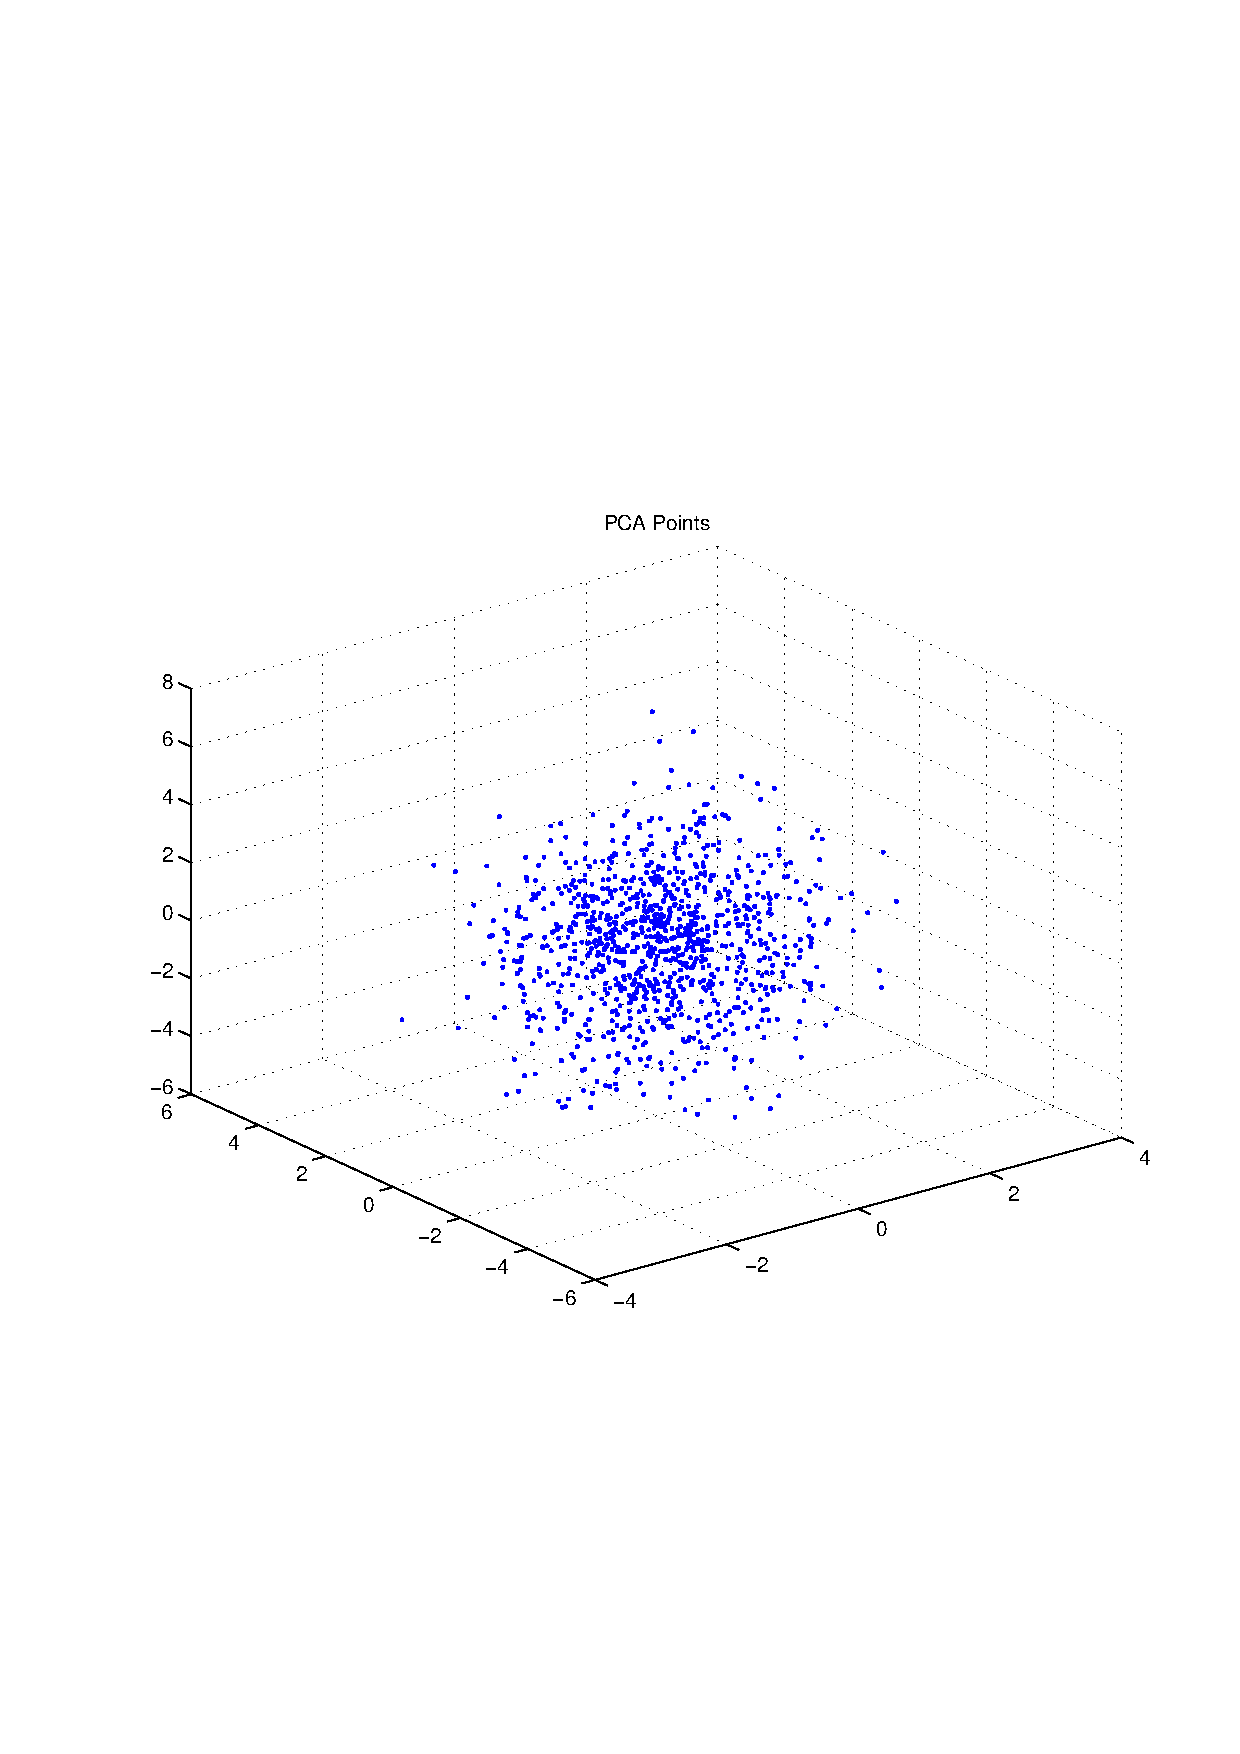
\includegraphics[width=10.0cm,height=10.0cm]{PCAPoints.pdf}

The eigenvectors:
+0.062, +0.163, +0.985
+0.217, +0.961, -0.173
-0.974, +0.225, +0.024

All of the eigenvalues of the covariance matrix:
(+0.958,+0.000), (+2.025,+0.000), (+3.017,+0.000)

QueryPerformanceCounter  =  +1.034
\subsubsection{Multi Variate Random Number Generator }
Sample from $N(\mu,\Sigma)$
mean= -0.002, variance=+1.004, skewness=+0.006, kurtosis=+3.003
mean= -0.001, variance=+1.017, skewness=-0.005, kurtosis=+2.988
mean= -0.002, variance=+1.006, skewness=-0.016, kurtosis=+3.014
Covariance Matrix 
+1.004, +0.009, +0.003
+0.009, +1.017, -0.003
+0.003, -0.003, +1.006

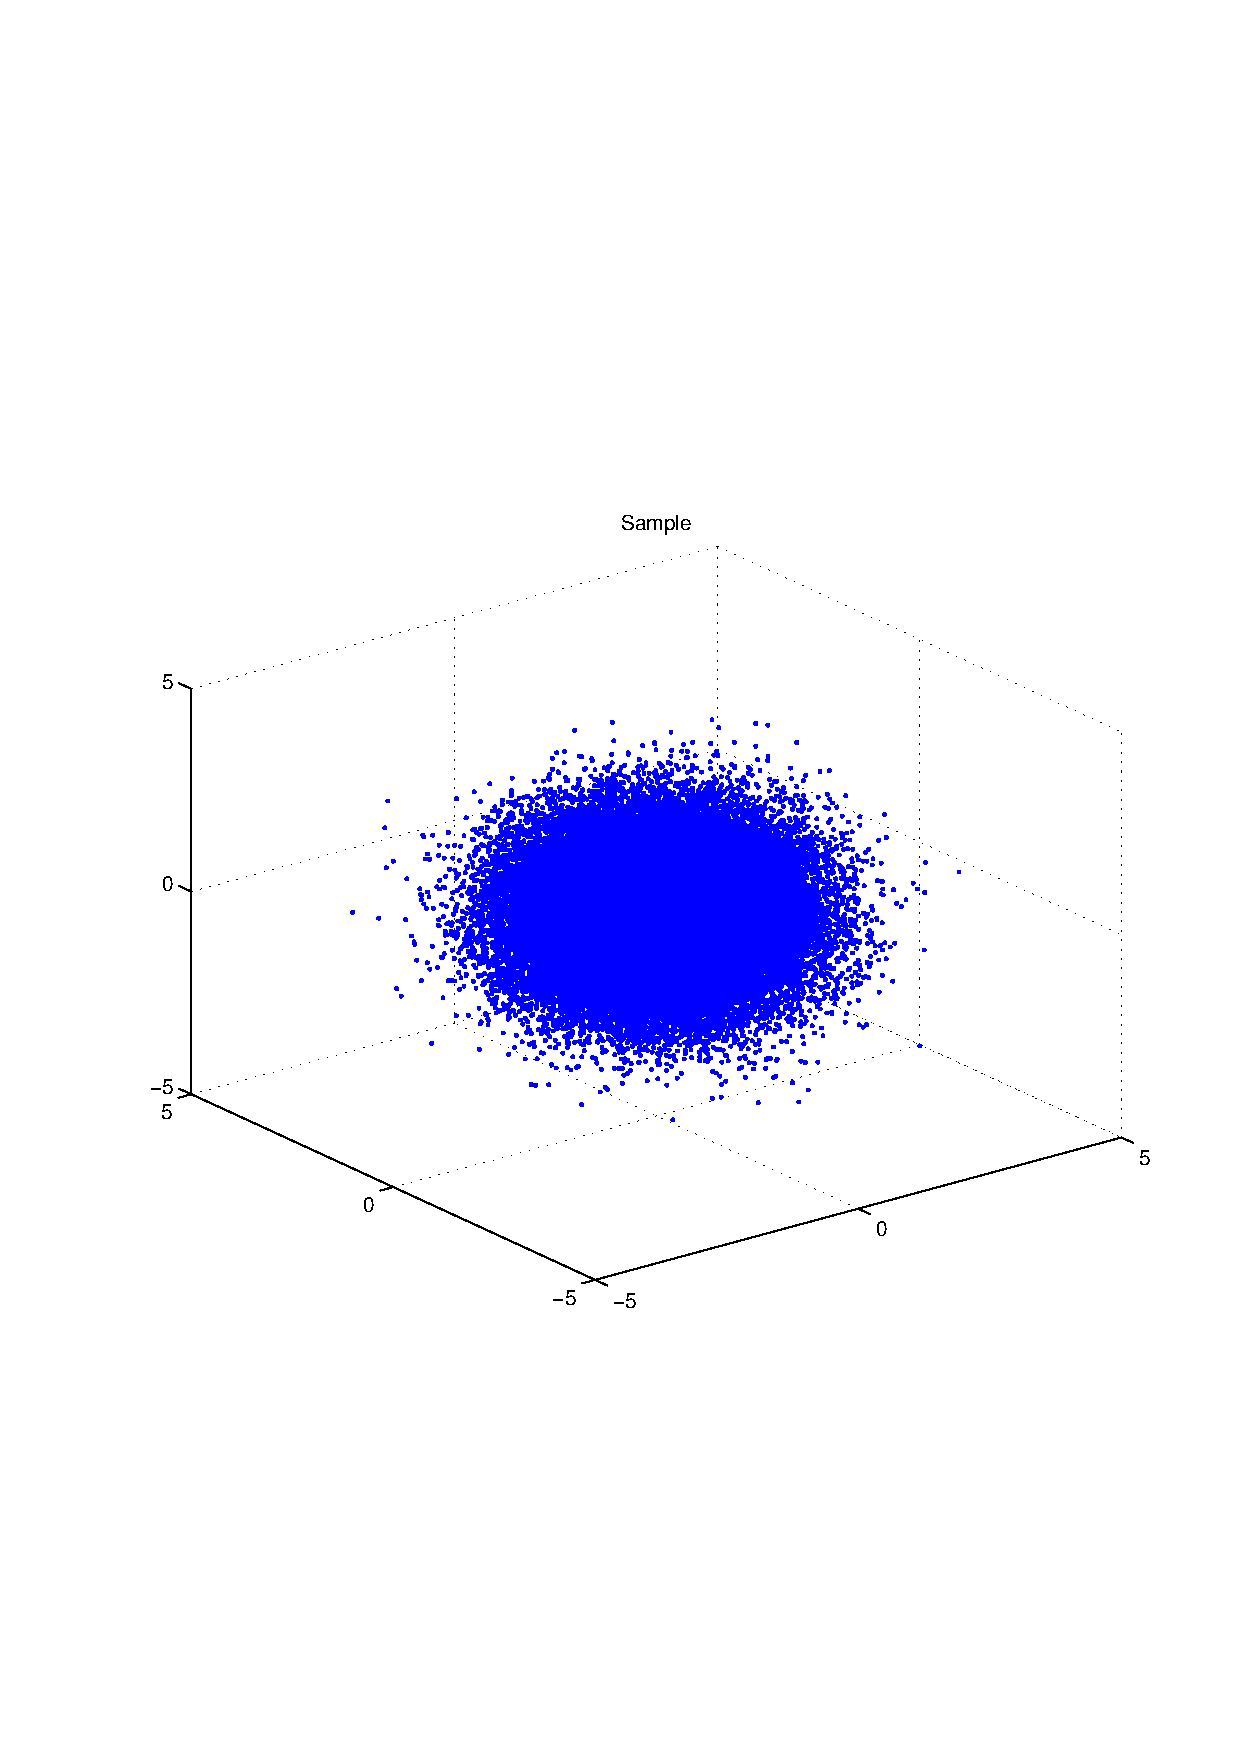
\includegraphics[width=10.0cm,height=10.0cm]{R_3_Normal.pdf}

Generate a sample from a unifom mixture of three Gaussians in $R^3$
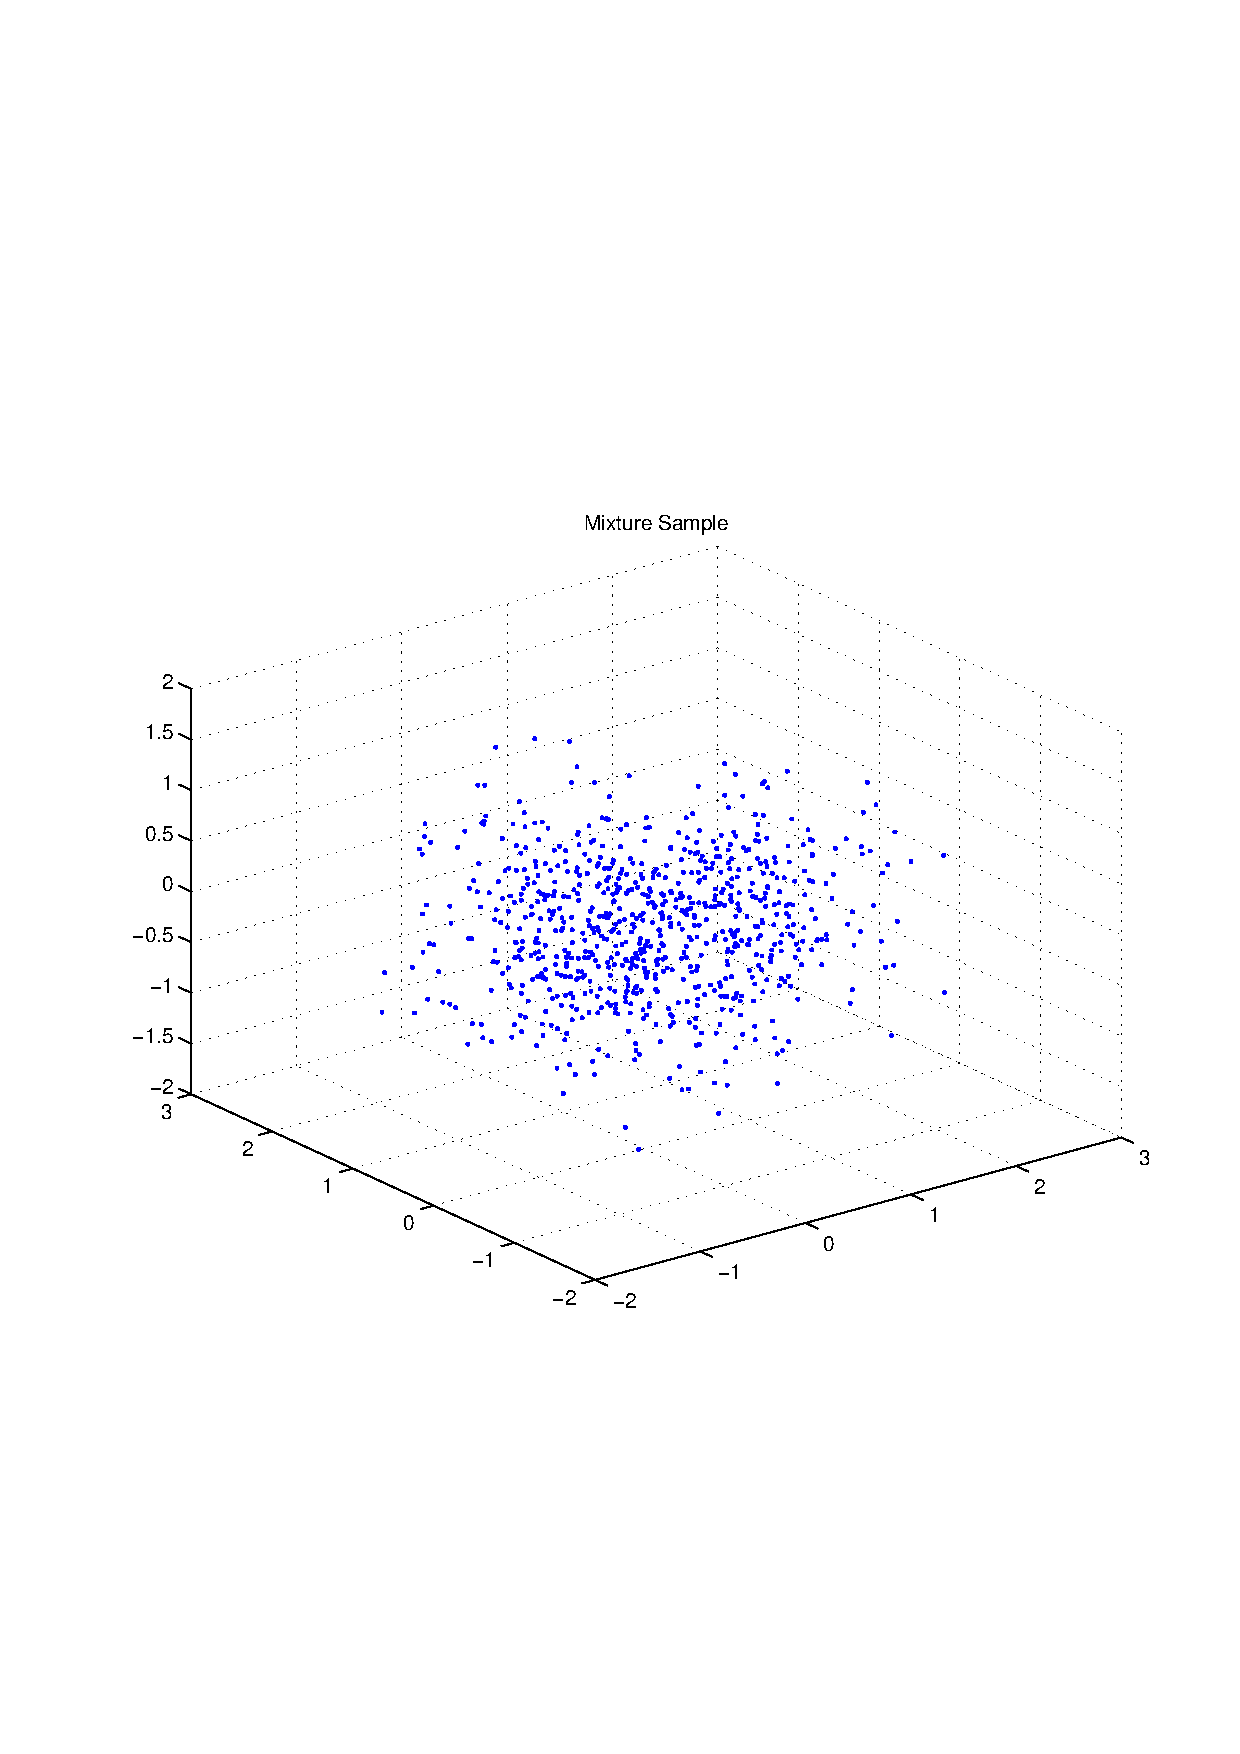
\includegraphics[width=10.0cm,height=10.0cm]{R_3_Normal_Mixture.pdf}

QueryPerformanceCounter  =  +15.477
\subsubsection{Matrix Multiply}
Comparing naive matrix multiply verus Intel MKL dgemm for matrix of size +2048.
This is for type double (hence the d in dgemm).
Naive type double matrix multiply tic toc  =  +0.352
dgemm plus row to column major transpose operation tic toc  =  +0.342
Comparing naive matrix multiply verus Intel MKL sgemm for matrix of size +2048.
This is for type float (hence the s in dgemm).
Naive type float matrix multiply tic toc  =  +0.258
sgemm plus row to column major transpose operation tic toc  =  +0.199
QueryPerformanceCounter  =  +1.291
\subsubsection{Descriptive Statistics}
Mean N(0,1): +0.003
Variance N(0,1): +1.006
Mean N(0,1) [recurrence relation method] :+0.003
Variance [recurrence relation method] :+1.006
Skewness : +0.007
Kurtosis : +2.997
QueryPerformanceCounter  =  +0.019
\subsubsection{Time Series }
+0.093
+0.726
+0.011
+2.178
QueryPerformanceCounter  =  +0.028
QueryPerformanceCounter  =  +5.960
\subsubsection{Iterated Exponential Filtering }
$\mu_1 =+0.093$
$\mu_2 =+0.726$
$\mu_3 =+0.011$
$\mu_4 =+2.178$
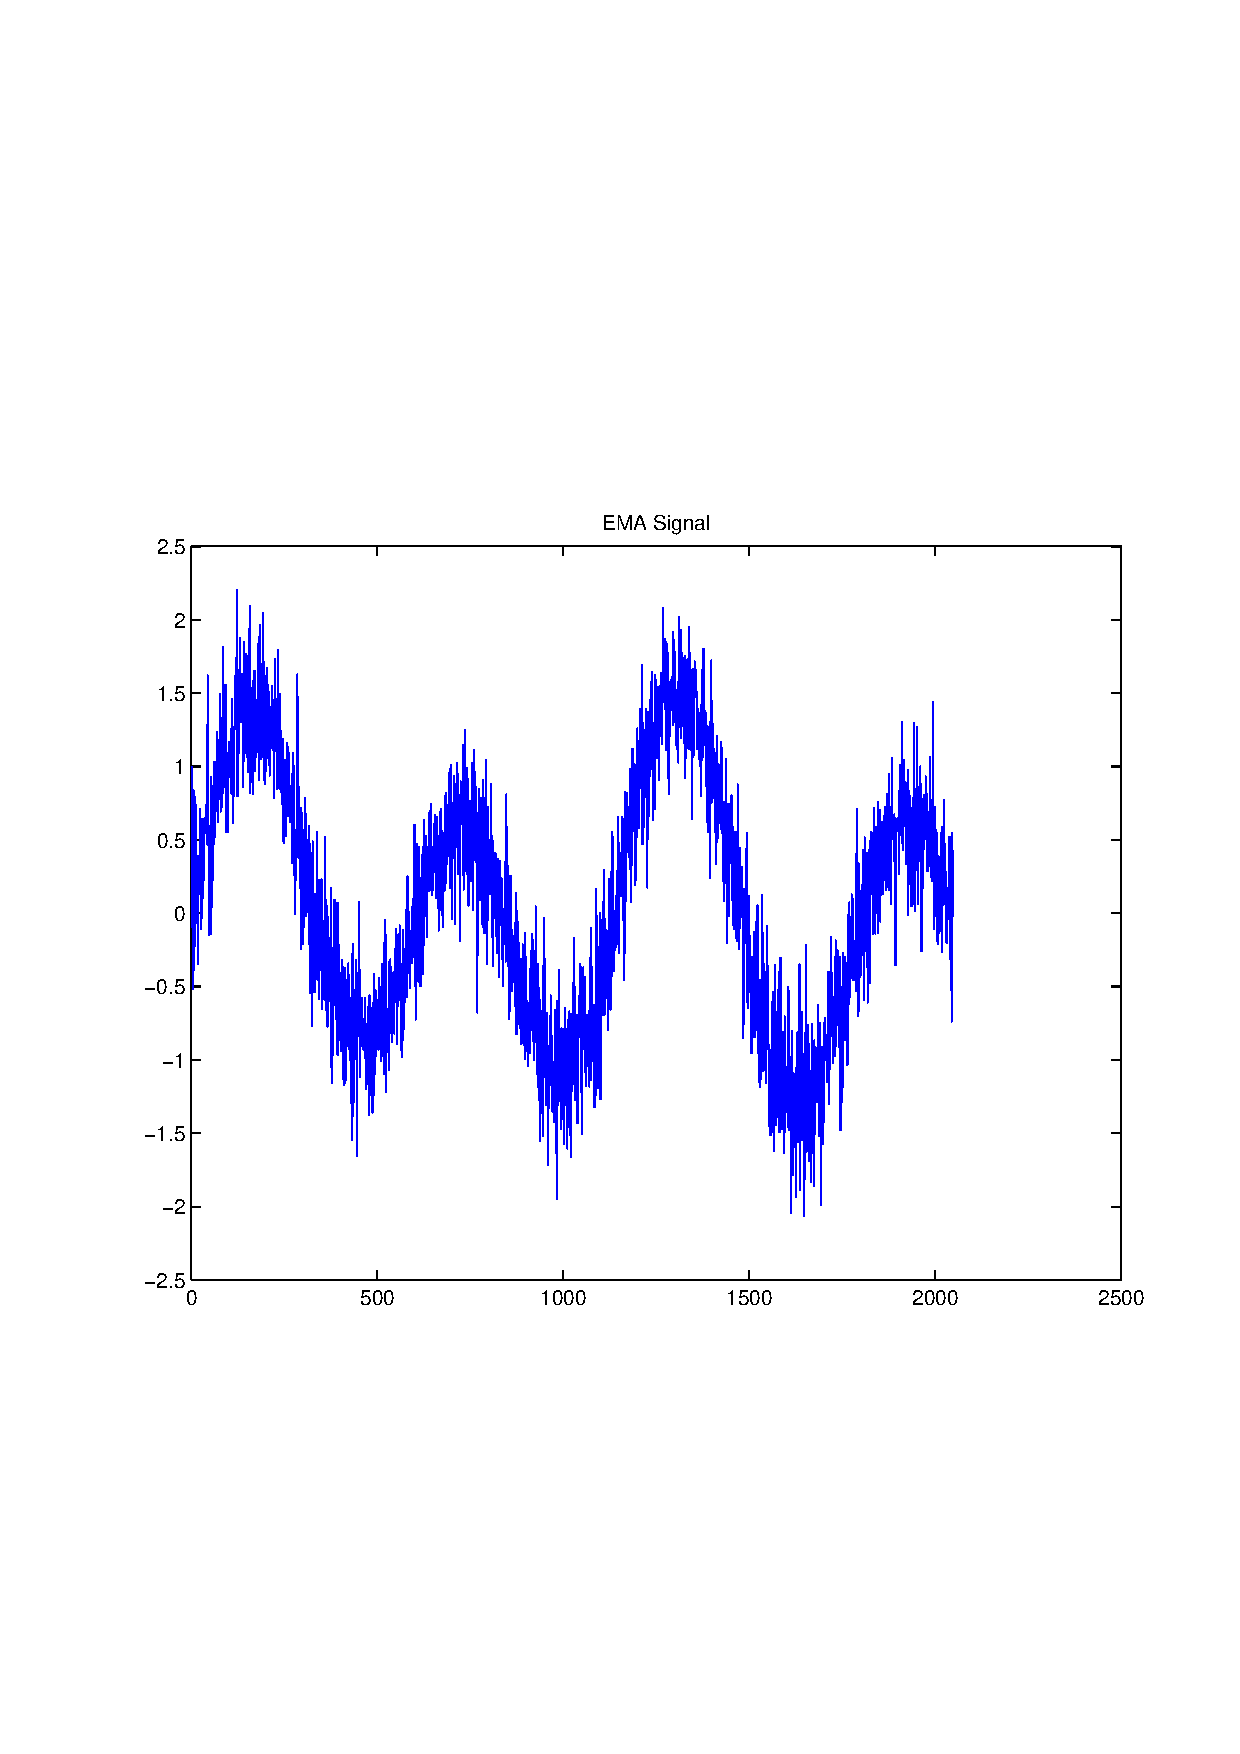
\includegraphics[width=10.0cm,height=10.0cm]{EMA_signal.pdf}

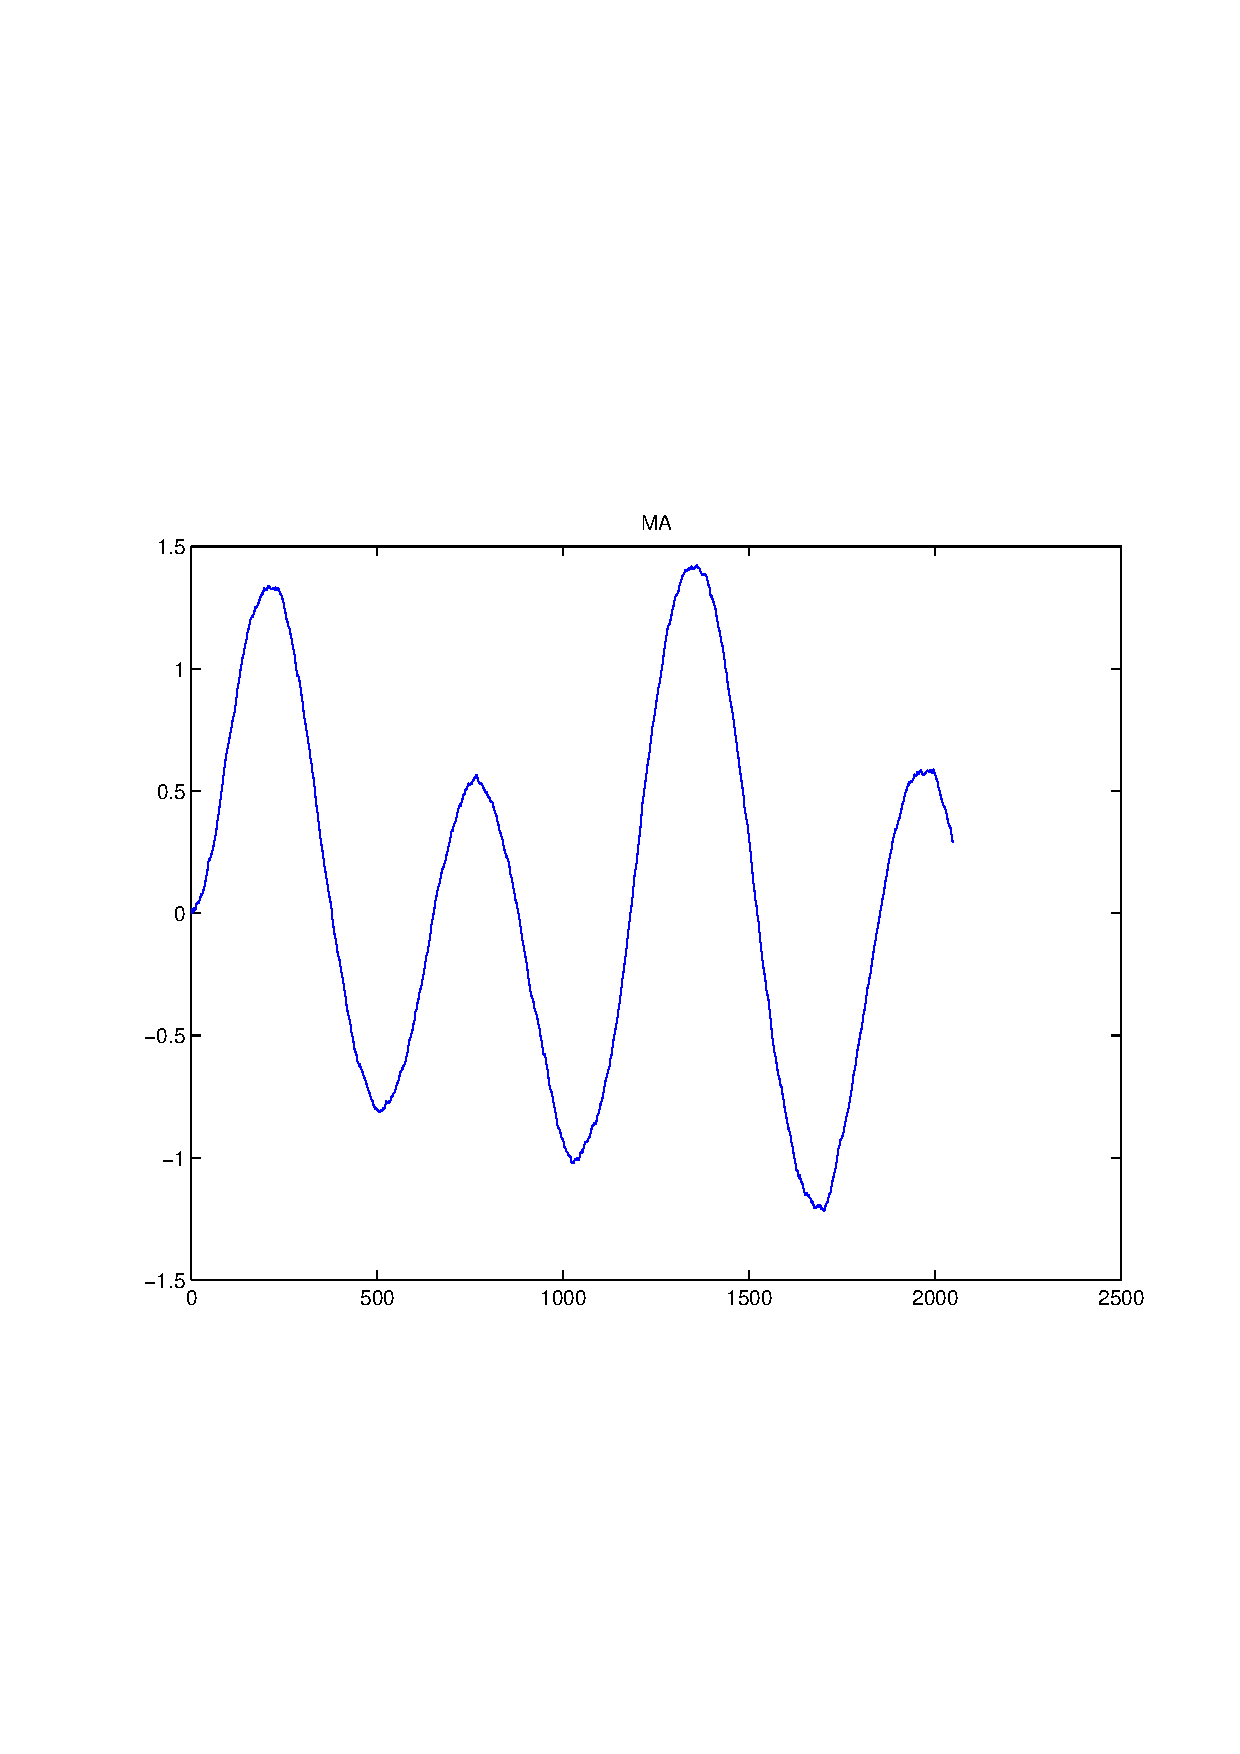
\includegraphics[width=10.0cm,height=10.0cm]{MA.pdf}

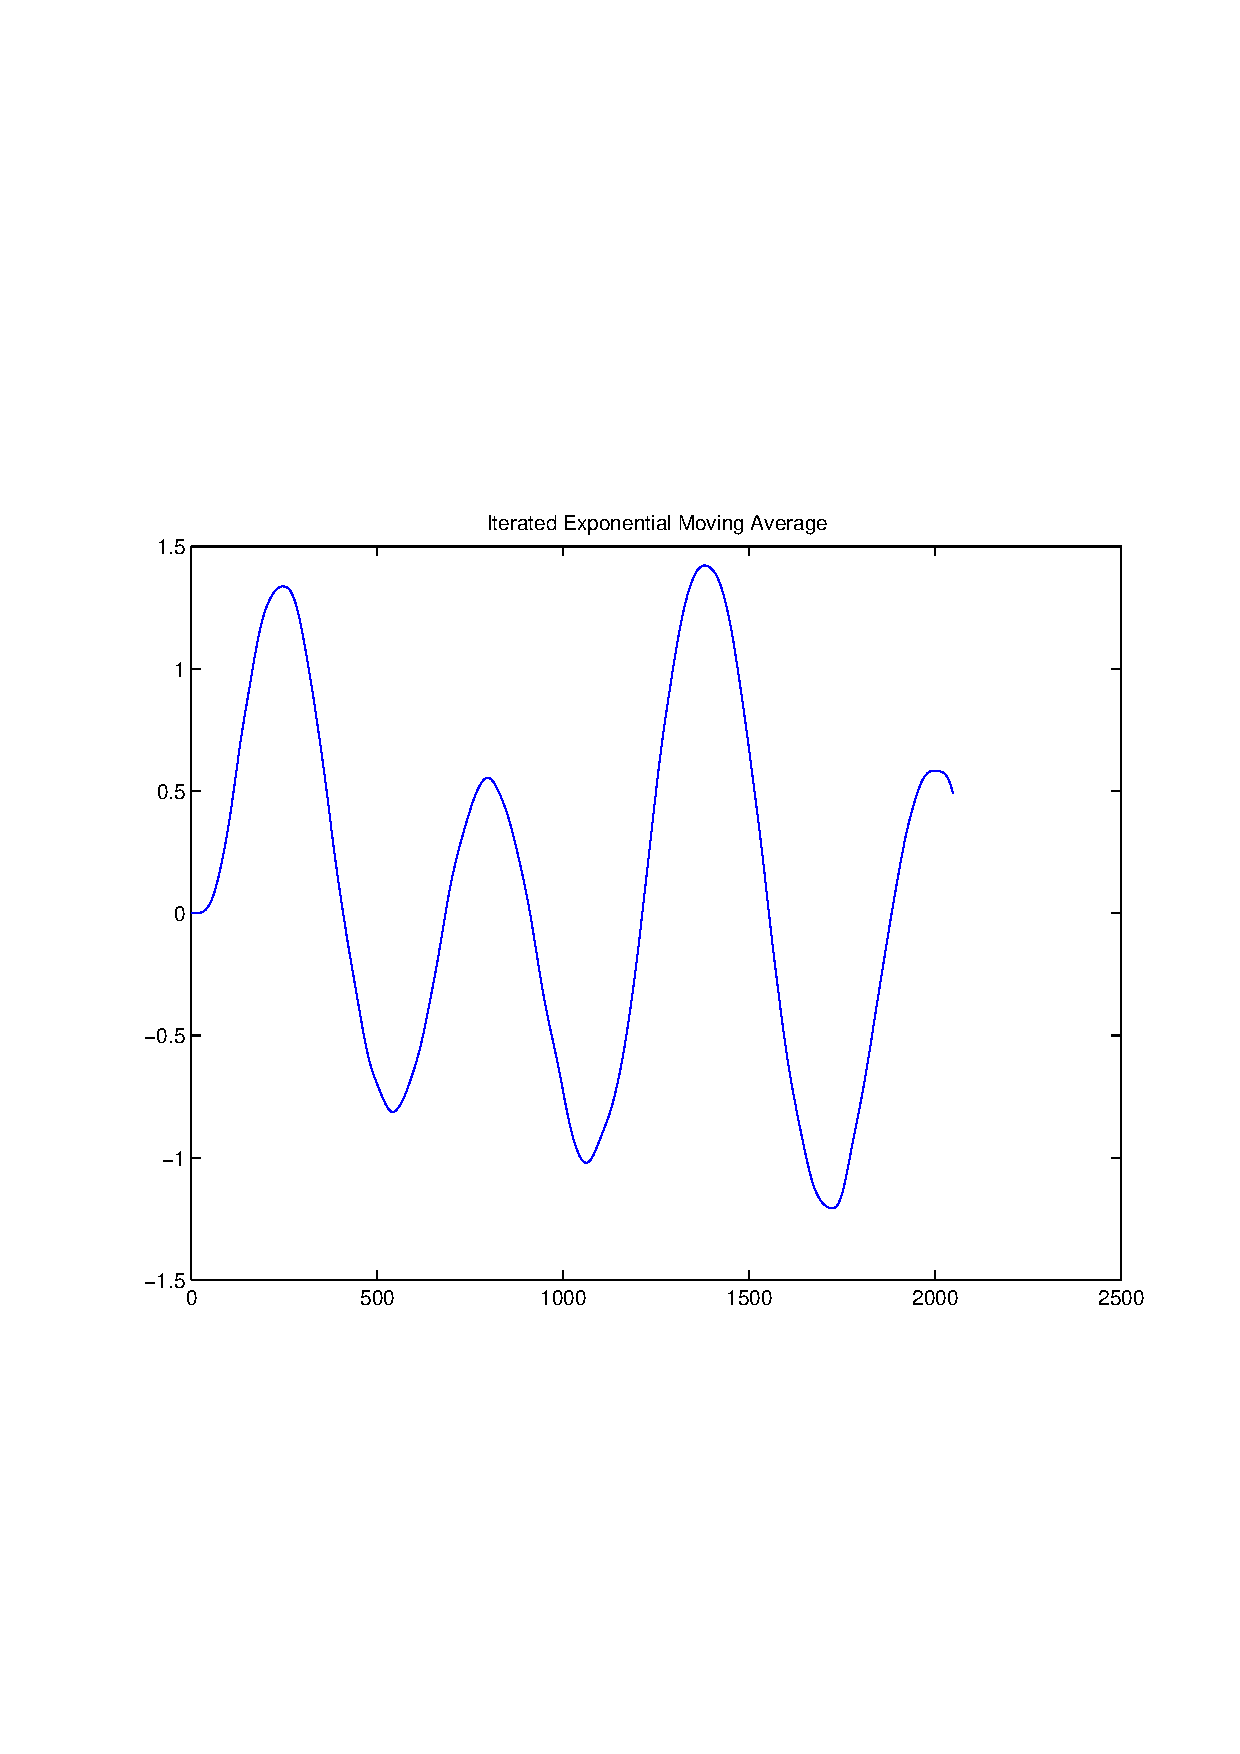
\includegraphics[width=10.0cm,height=10.0cm]{IEMA.pdf}

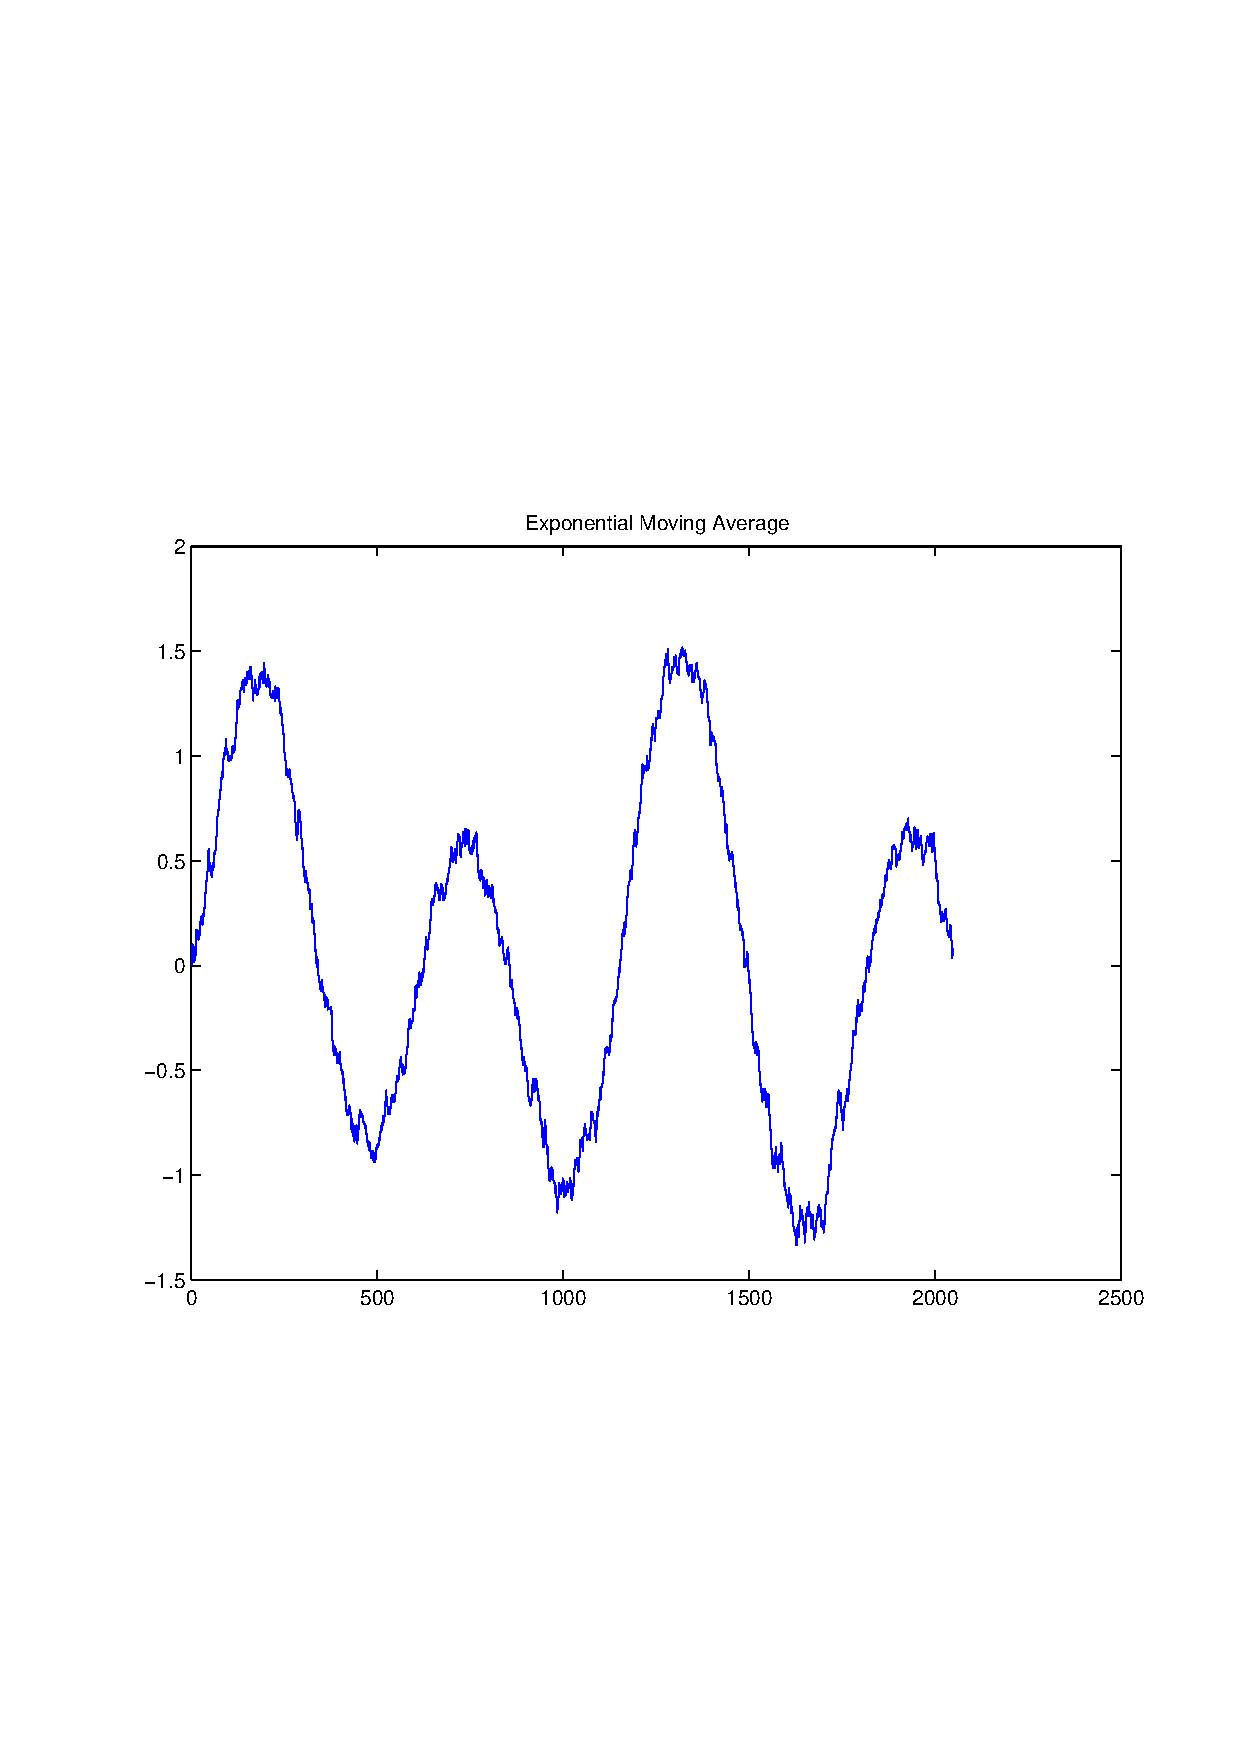
\includegraphics[width=10.0cm,height=10.0cm]{EMA.pdf}

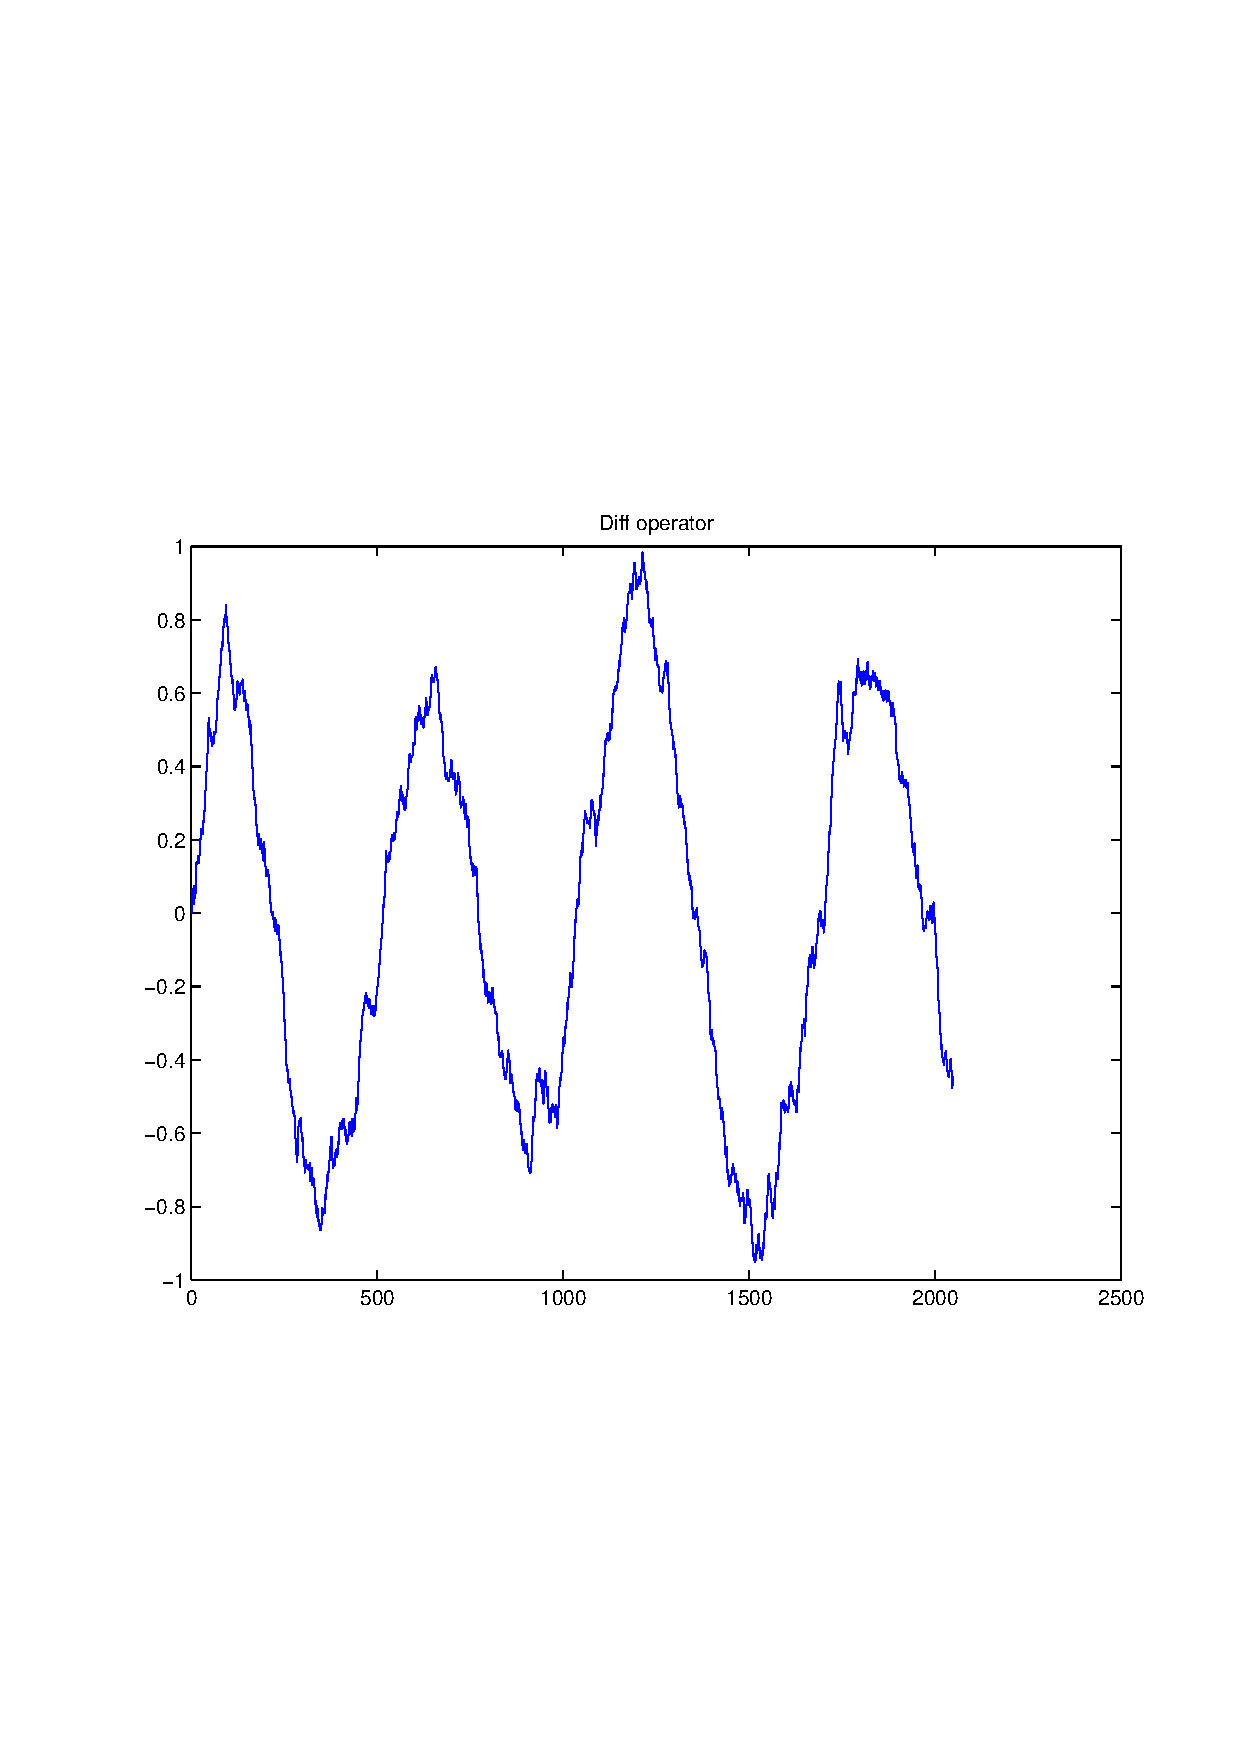
\includegraphics[width=10.0cm,height=10.0cm]{DIFF.pdf}

\includegraphics[width=10.0cm,height=10.0cm]{IteratedExponentailOperators.pdf}

\includegraphics[width=10.0cm,height=10.0cm]{IteratedExponentailOperators.pdf}

QueryPerformanceCounter  =  +7.701
\subsubsection{Testing binary writer}
Binary writer Speedup 1GB Double Matrix +46.918

Binary reader Speedup 1GB Double Matrix +197.202

Binary writer Speedup 1GB Double vector +38.441

Binary reader Speedup 1GB Double Matrix +148.522

QueryPerformanceCounter  =  +0.814
\subsubsection{Testing Gaussian Mixture Point Cloud and Latex Plotting Capabilities.}
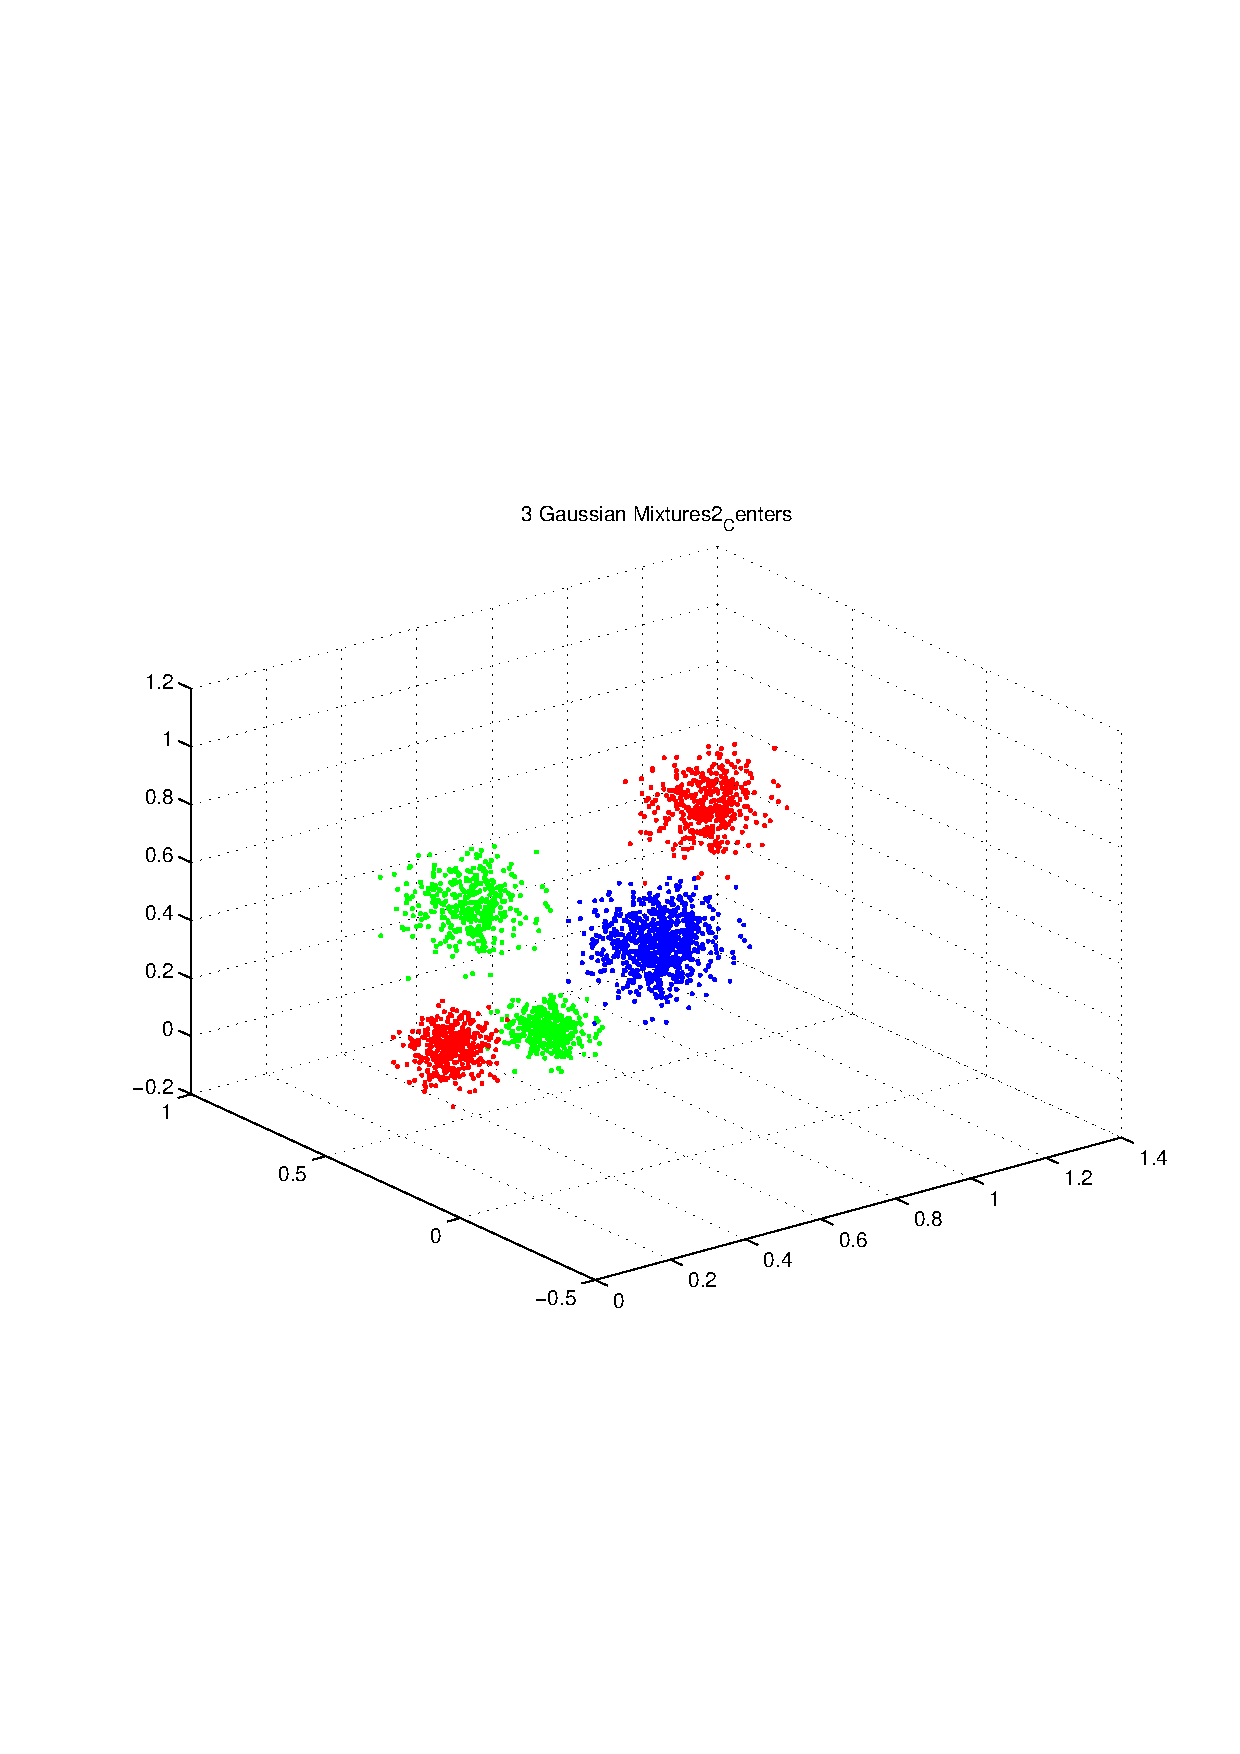
\includegraphics[width=10.0cm,height=10.0cm]{GaussianMixture_Dim_3_Centers2.pdf}

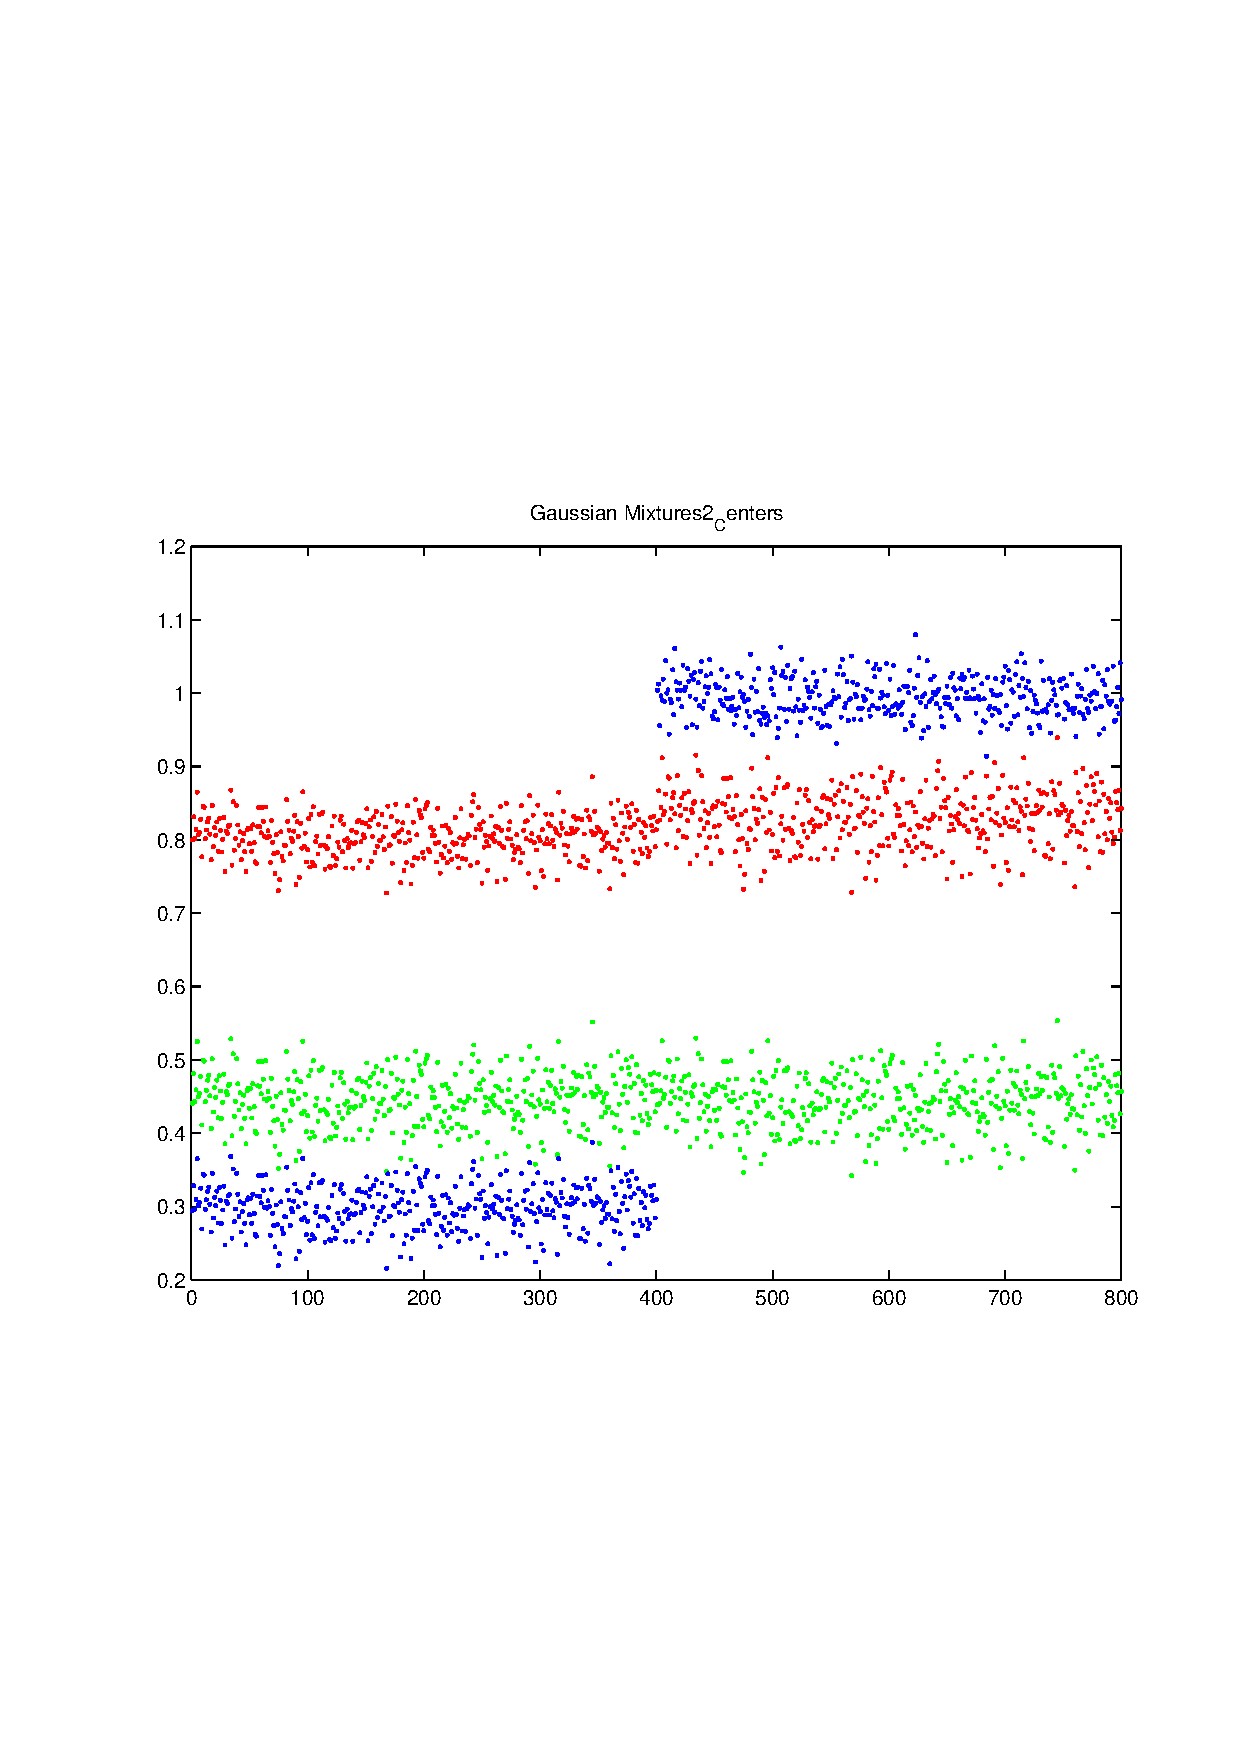
\includegraphics[width=10.0cm,height=10.0cm]{GaussianMixture_Dim_1_Centers2.pdf}

QueryPerformanceCounter  =  +2.798
\subsubsection{Intel VSL Function Check}
\includegraphics[width=10.0cm,height=10.0cm]{klVSLInv.pdf}

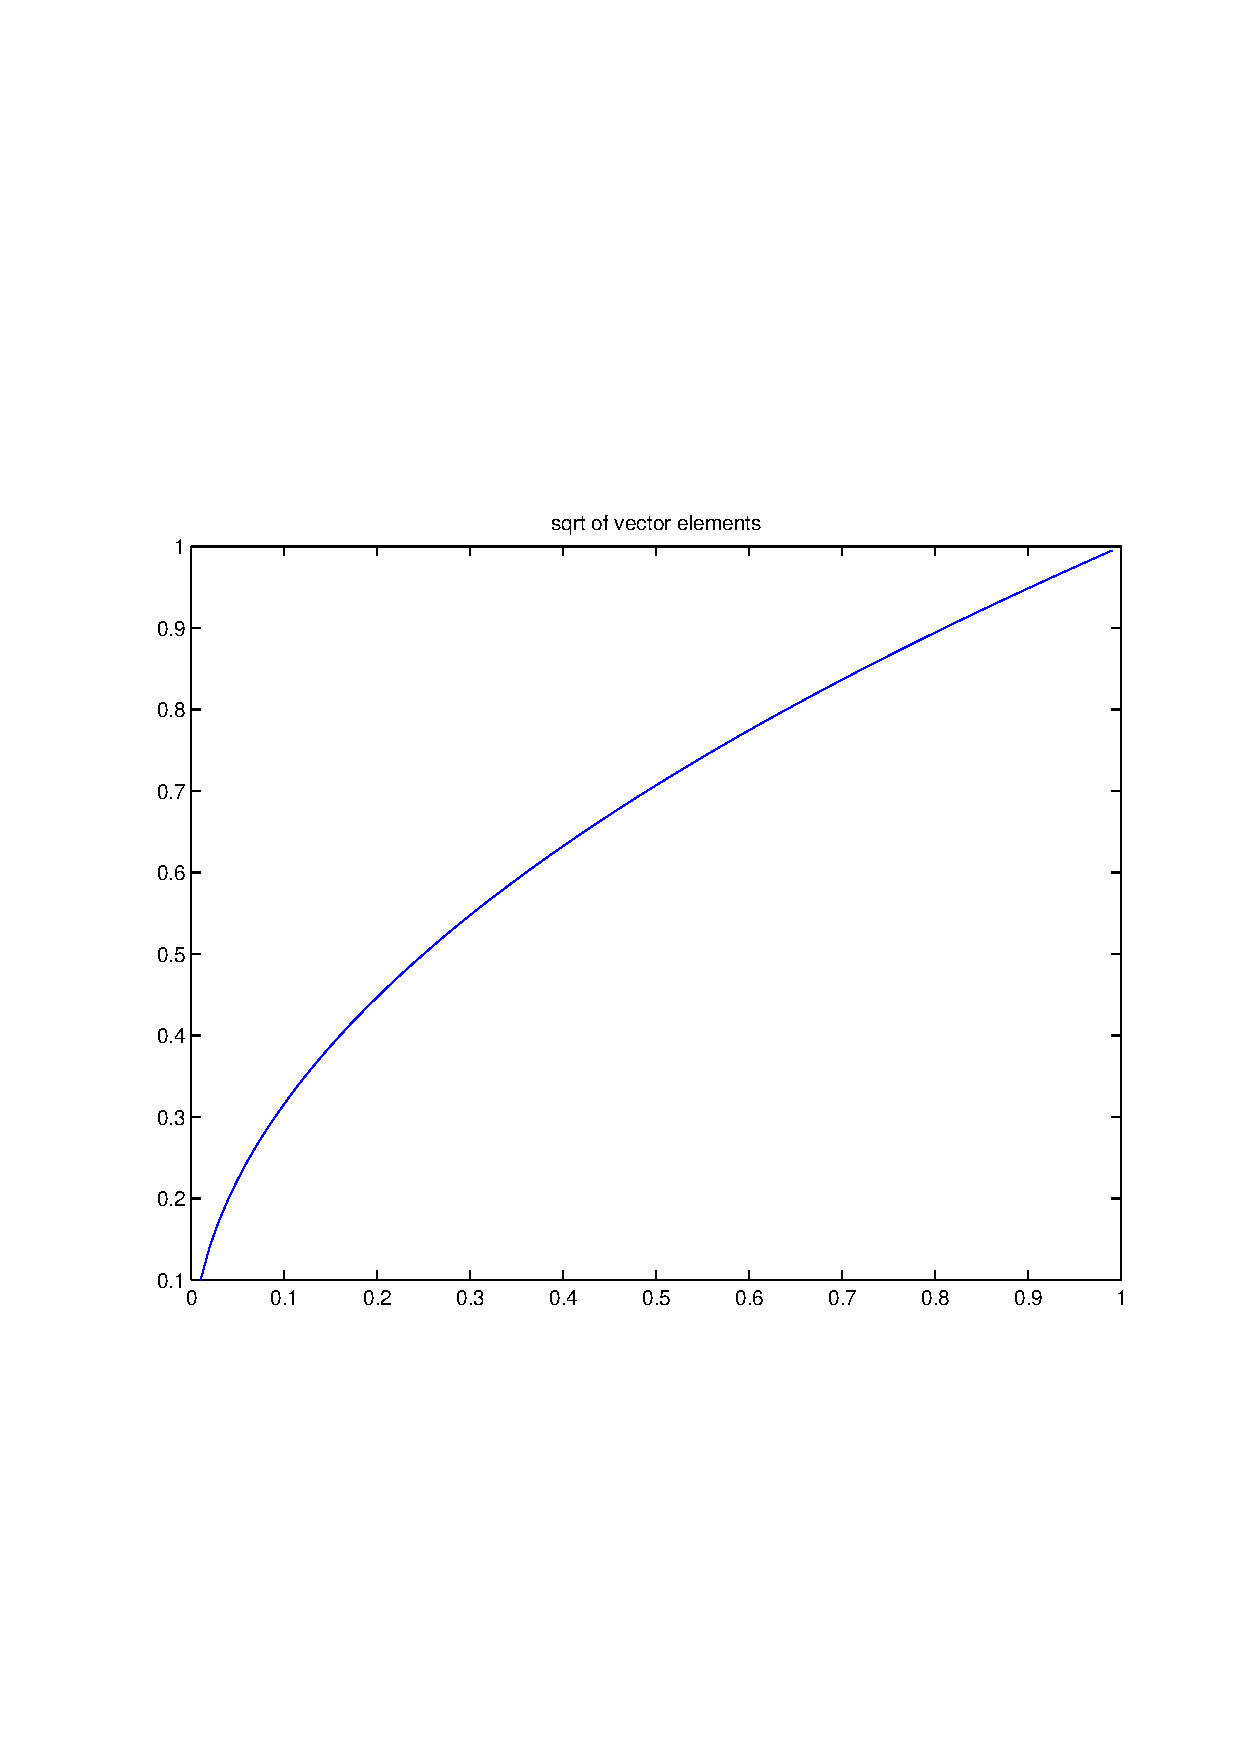
\includegraphics[width=10.0cm,height=10.0cm]{klVSLSqrt.pdf}

\includegraphics[width=10.0cm,height=10.0cm]{klVSLExp.pdf}

\includegraphics[width=10.0cm,height=10.0cm]{klVSLExpm1.pdf}

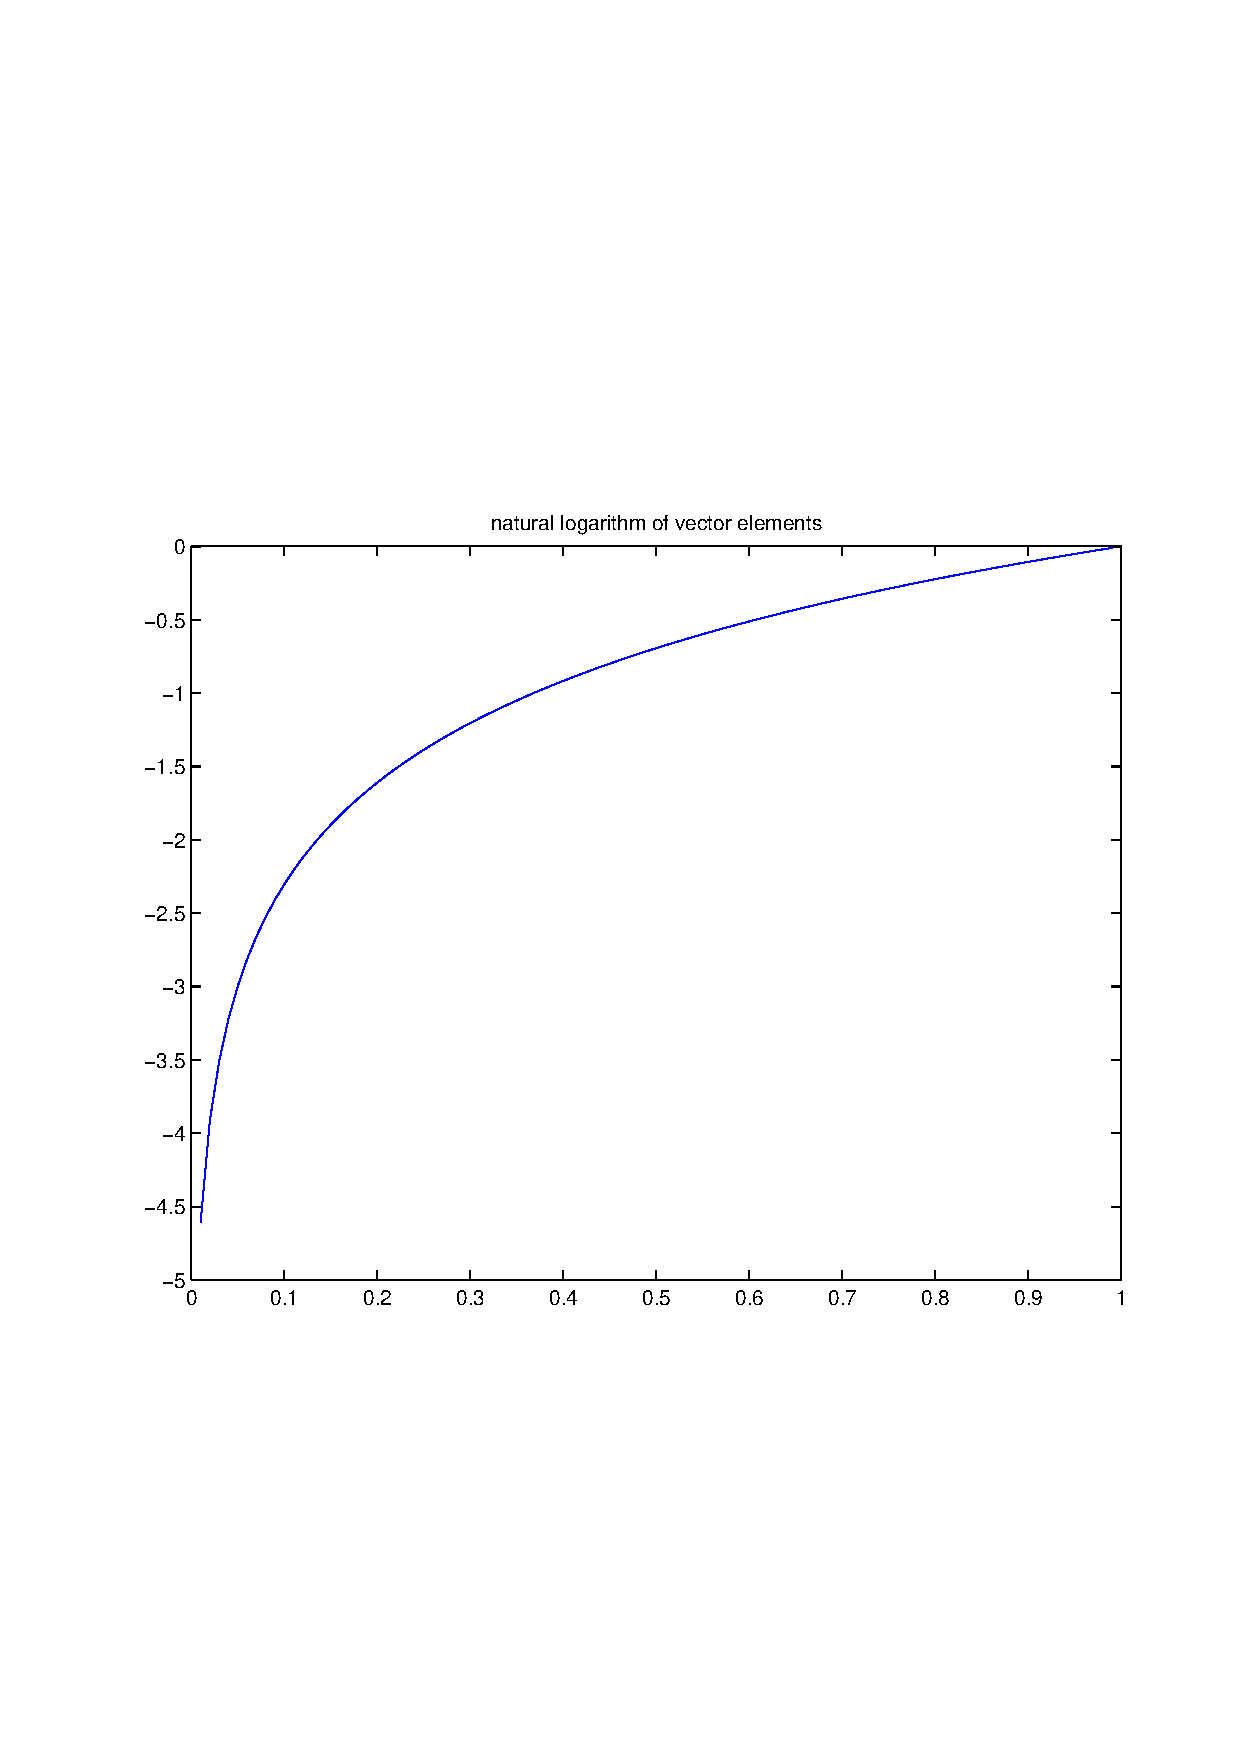
\includegraphics[width=10.0cm,height=10.0cm]{klVSLLn.pdf}

\includegraphics[width=10.0cm,height=10.0cm]{klVSLLog10.pdf}

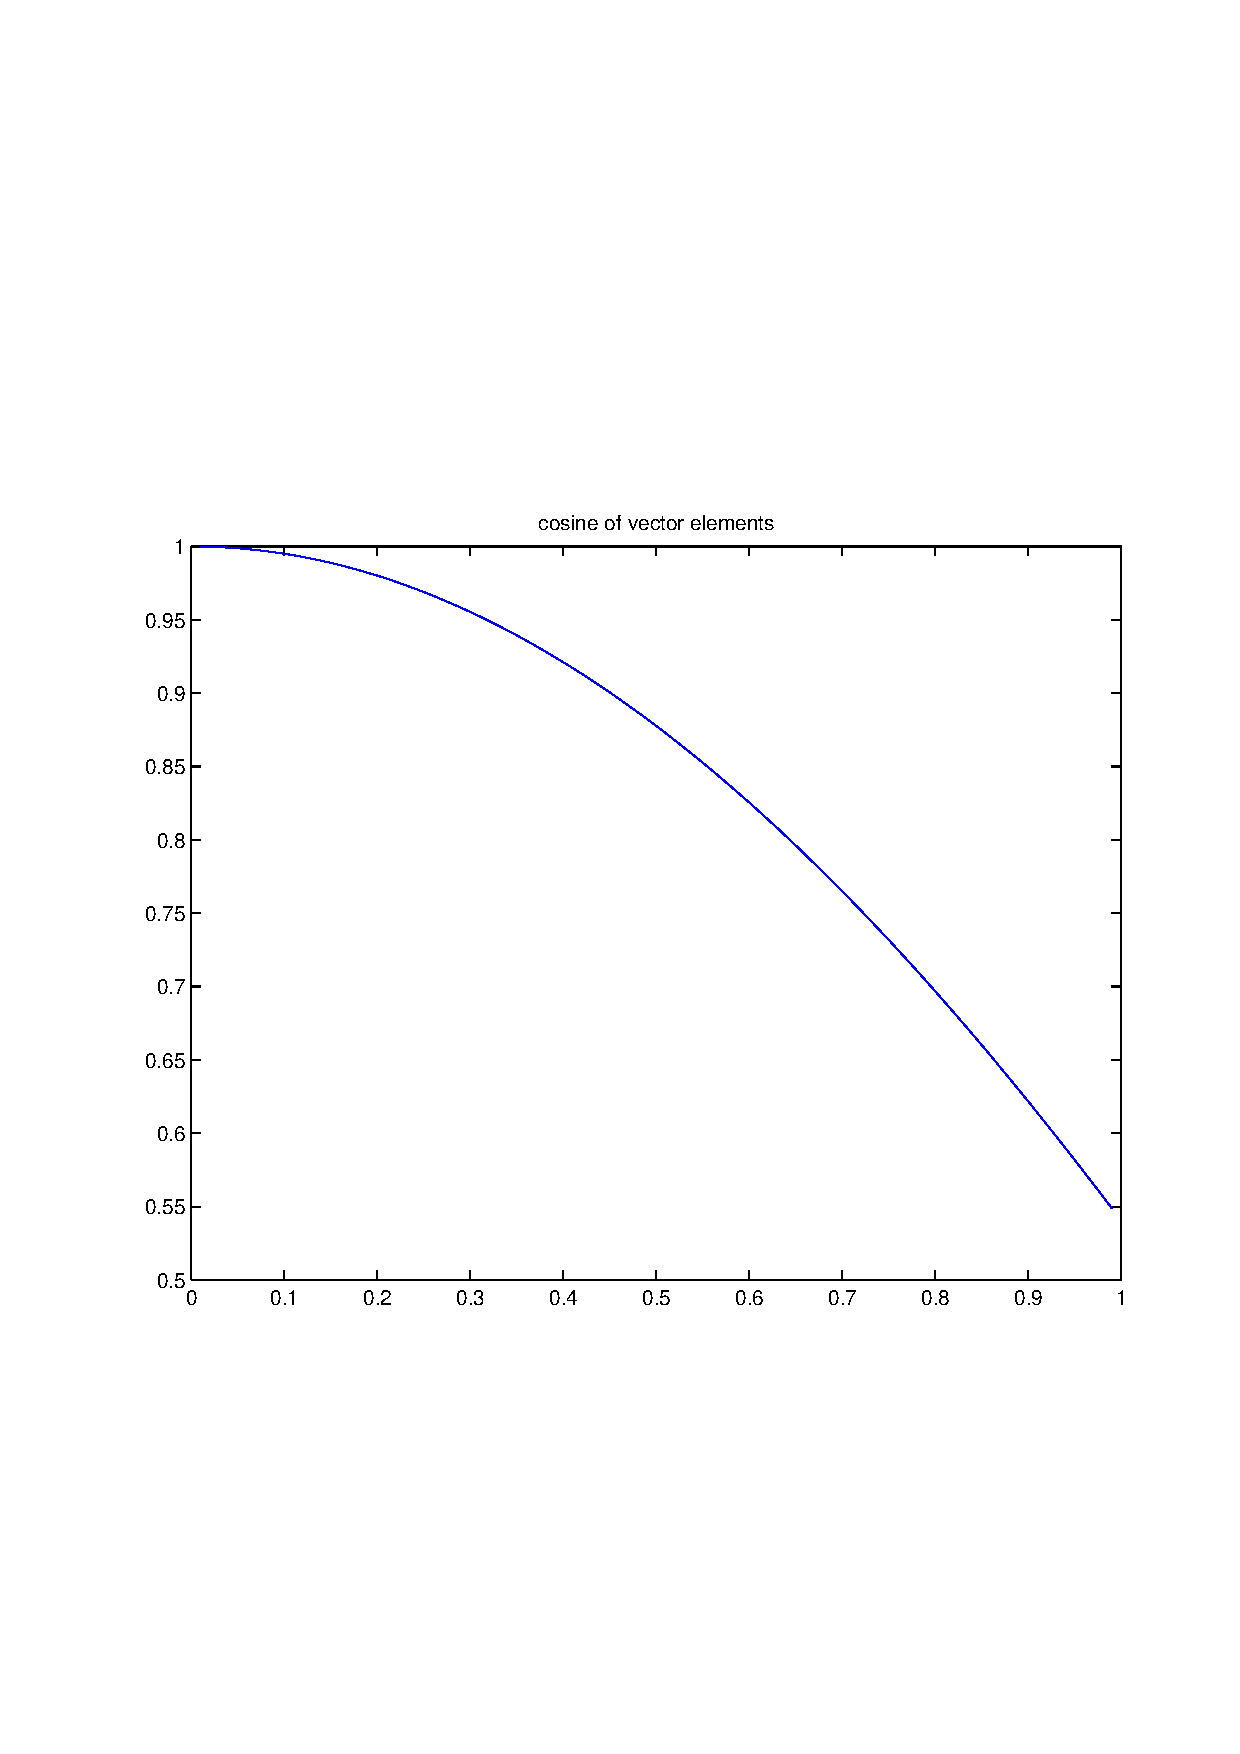
\includegraphics[width=10.0cm,height=10.0cm]{klVSLCos.pdf}

\includegraphics[width=10.0cm,height=10.0cm]{klVSLSin.pdf}

\includegraphics[width=10.0cm,height=10.0cm]{klVSLTan.pdf}

\includegraphics[width=10.0cm,height=10.0cm]{klVSLErf.pdf}

\includegraphics[width=10.0cm,height=10.0cm]{klVSLErfc.pdf}

\includegraphics[width=10.0cm,height=10.0cm]{klVSLCdfNorm.pdf}

\includegraphics[width=10.0cm,height=10.0cm]{klVSLErfInv.pdf}

\includegraphics[width=10.0cm,height=10.0cm]{klVSLLGamma.pdf}

\includegraphics[width=10.0cm,height=10.0cm]{klVSLTGamma.pdf}

QueryPerformanceCounter  =  +15.203
\subsubsection{Gram Matrix Consistency Check}
Sample Size = 4096
Feature dim = 3

$$Sigma$ = \left(
\begin{array}{
ccc}
+1.140 & +1.535 & +0.581 \\
+1.535 & +9.988 & +1.605 \\
+0.581 & +1.605 & +0.428 \\
\end{array}
\right)$ \newline 

$Sample Covariance = \left(
\begin{array}{
ccc}
+1.122 & +1.441 & +0.560 \\
+1.441 & +10.142 & +1.561 \\
+0.560 & +1.561 & +0.411 \\
\end{array}
\right)$ \newline 

$Sample Mean = \left(
\begin{array}{
ccc}
+1.00934 & +0.99120 & +1.00107 \\
\end{array}
\right)$ \newline 

$Sample Covariance-$Omega$ = \left(
\begin{array}{
ccc}
-0.018 & -0.094 & -0.021 \\
-0.094 & +0.154 & -0.044 \\
-0.021 & -0.044 & -0.016 \\
\end{array}
\right)$ \newline 

$Sample Covariance Eigs = \left(
\begin{array}{
ccc}
(+10.62661,+0.00000) & (+1.00815,+0.00000) & (+0.04023,+0.00000) \\
\end{array}
\right)$ \newline 

$Centered Mean = \left(
\begin{array}{
ccc}
-0.00000 & -0.00000 & +0.00000 \\
\end{array}
\right)$ \newline 

$Centered Covariance = \left(
\begin{array}{
ccc}
+1.122 & +1.441 & +0.560 \\
+1.441 & +10.142 & +1.561 \\
+0.560 & +1.561 & +0.411 \\
\end{array}
\right)$ \newline 

$Gram Matrix Gf Not scaled by sample size = \left(
\begin{array}{
ccc}
+4594.197 & +5901.907 & +2293.420 \\
+5901.907 & +41541.271 & +6393.634 \\
+2293.420 & +6393.634 & +1685.301 \\
\end{array}
\right)$ \newline 

$Gram Matrix Gf  scaled by sample size = \left(
\begin{array}{
ccc}
+1.122 & +1.441 & +0.560 \\
+1.441 & +10.142 & +1.561 \\
+0.560 & +1.561 & +0.411 \\
\end{array}
\right)$ \newline 

$SampleCovariance - Scaled Gf = \left(
\begin{array}{
ccc}
+0.000 & +0.000 & +0.000 \\
+0.000 & +0.002 & +0.000 \\
+0.000 & +0.000 & +0.000 \\
\end{array}
\right)$ \newline 

$EigenDecomp of SampleCovariance = \left(
\begin{array}{
ccc}
-0.157 & -0.975 & -0.158 \\
+0.920 & -0.202 & +0.334 \\
-0.358 & -0.093 & +0.929 \\
\end{array}
\right)$ \newline 

$EigenDecomp of Gram Matrix = \left(
\begin{array}{
ccc}
-0.100 & -0.979 & -0.179 \\
-0.255 & +0.199 & -0.946 \\
+0.962 & -0.049 & -0.270 \\
\end{array}
\right)$ \newline 

QueryPerformanceCounter  =  +1.378
\subsubsection{Eigen Solver Checks}
\subsubsection{Haar Distributed Random Orthogonal Matrix $A \in O(n)$}
 Testing Operator Norm
Number of Dimensions: +8

$A = \left(
\begin{array}{
cccccccc}
-0.114 & -0.445 & +0.446 & +0.119 & -0.697 & +0.046 & -0.295 & -0.030 \\
+0.182 & +0.328 & -0.375 & -0.212 & -0.527 & +0.593 & +0.101 & +0.188 \\
-0.792 & -0.211 & -0.177 & -0.084 & -0.086 & +0.013 & +0.516 & +0.126 \\
+0.028 & -0.241 & -0.638 & +0.601 & -0.098 & -0.009 & -0.098 & -0.392 \\
+0.281 & +0.193 & +0.223 & +0.561 & -0.202 & -0.228 & +0.574 & +0.311 \\
+0.024 & +0.203 & -0.303 & -0.330 & -0.398 & -0.769 & -0.087 & +0.004 \\
+0.466 & -0.531 & -0.023 & -0.386 & -0.016 & -0.001 & +0.502 & -0.315 \\
-0.171 & +0.480 & +0.283 & +0.007 & -0.142 & +0.054 & +0.196 & -0.773 \\
\end{array}
\right)$ \newline 

$Det(A) :   A \in O(n)$ = (+1.000,+0.000)

$L = \left(
\begin{array}{
cccccccc}
+1.000 & +0.000 & +0.000 & +0.000 & +0.000 & +0.000 & +0.000 & +0.000 \\
-0.589 & +1.000 & +0.000 & +0.000 & +0.000 & +0.000 & +0.000 & +0.000 \\
-0.036 & +0.380 & +1.000 & +0.000 & +0.000 & +0.000 & +0.000 & +0.000 \\
+0.143 & +0.633 & -0.927 & +1.000 & +0.000 & +0.000 & +0.000 & +0.000 \\
-0.229 & -0.426 & +0.789 & -0.914 & +1.000 & +0.000 & +0.000 & +0.000 \\
-0.030 & -0.299 & +0.582 & -0.814 & +0.820 & +1.000 & +0.000 & +0.000 \\
-0.355 & -0.180 & -0.231 & +0.564 & -0.120 & +0.132 & +1.000 & +0.000 \\
+0.216 & -0.802 & -0.368 & -0.039 & +0.200 & +0.058 & +0.403 & +1.000 \\
\end{array}
\right)$ \newline 

$U = \left(
\begin{array}{
cccccccc}
-0.792 & -0.211 & -0.177 & -0.084 & -0.086 & +0.013 & +0.516 & +0.126 \\
+0.000 & -0.656 & -0.128 & -0.435 & -0.067 & +0.006 & +0.805 & -0.241 \\
+0.000 & +0.000 & -0.596 & +0.764 & -0.075 & -0.011 & -0.385 & -0.296 \\
+0.000 & +0.000 & +0.000 & +1.114 & -0.712 & +0.030 & -1.235 & -0.170 \\
+0.000 & +0.000 & +0.000 & +0.000 & -1.166 & +0.635 & -0.262 & +0.192 \\
+0.000 & +0.000 & +0.000 & +0.000 & +0.000 & -1.256 & -0.396 & -0.188 \\
+0.000 & +0.000 & +0.000 & +0.000 & +0.000 & +0.000 & +1.531 & +0.388 \\
+0.000 & +0.000 & +0.000 & +0.000 & +0.000 & +0.000 & +0.000 & -1.293 \\
\end{array}
\right)$ \newline 

$L * U  = \left(
\begin{array}{
cccccccc}
-0.792 & -0.211 & -0.177 & -0.084 & -0.086 & +0.013 & +0.516 & +0.126 \\
+0.466 & -0.531 & -0.023 & -0.386 & -0.016 & -0.001 & +0.502 & -0.315 \\
+0.028 & -0.241 & -0.638 & +0.601 & -0.098 & -0.009 & -0.098 & -0.392 \\
-0.114 & -0.445 & +0.446 & +0.119 & -0.697 & +0.046 & -0.295 & -0.030 \\
+0.182 & +0.328 & -0.375 & -0.212 & -0.527 & +0.593 & +0.101 & +0.188 \\
+0.024 & +0.203 & -0.303 & -0.330 & -0.398 & -0.769 & -0.087 & +0.004 \\
+0.281 & +0.193 & +0.223 & +0.561 & -0.202 & -0.228 & +0.574 & +0.311 \\
-0.171 & +0.480 & +0.283 & +0.007 & -0.142 & +0.054 & +0.196 & -0.773 \\
\end{array}
\right)$ \newline 

$Det(L) :    = (+1.000,+0.000)     Det(U) :    = (+1.000,+0.000)     Det(LU) :    = (+1.000,+0.000)$

$||A||_{L_1}$  = +2.633

$||A||_{L_{\infty}}$ = +2.574

$||A^{-1}||_{L_1}$  = +2.574

$||A^{-1}||_{L_{\infty}}$ = +2.633

$||A||_{L_{\infty}} * ||A^{-1}||_{L_{\infty}} = +6.777$

$||A||_{L_1} * ||A^{-1}||_{L_1} = +6.777$

Frobenious Norm  $||A||_{\textit{F}}$ via $\sum\limits_{i,j =0}^{n} \|A_{i,j}|$   of  $A \in O(n)$  +2.828

$L_1$ condition number of Haar Distributed Random Orthogonal Matrix $A \in O(n)$ +5.544

$A = \left(
\begin{array}{
cccccccc}
-0.114 & -0.445 & +0.446 & +0.119 & -0.697 & +0.046 & -0.295 & -0.030 \\
+0.182 & +0.328 & -0.375 & -0.212 & -0.527 & +0.593 & +0.101 & +0.188 \\
-0.792 & -0.211 & -0.177 & -0.084 & -0.086 & +0.013 & +0.516 & +0.126 \\
+0.028 & -0.241 & -0.638 & +0.601 & -0.098 & -0.009 & -0.098 & -0.392 \\
+0.281 & +0.193 & +0.223 & +0.561 & -0.202 & -0.228 & +0.574 & +0.311 \\
+0.024 & +0.203 & -0.303 & -0.330 & -0.398 & -0.769 & -0.087 & +0.004 \\
+0.466 & -0.531 & -0.023 & -0.386 & -0.016 & -0.001 & +0.502 & -0.315 \\
-0.171 & +0.480 & +0.283 & +0.007 & -0.142 & +0.054 & +0.196 & -0.773 \\
\end{array}
\right)$ \newline 

$L_{\infty}$ condition number of Haar Distributed Random Orthogonal Matrix $A \in O(n)$ +5.508

Eigenvalues of $A \in O(n)$

(+0.168,+0.986), (+0.168,-0.986), (-0.468,+0.884), (-0.468,-0.884), (-0.994,+0.110), (-0.994,-0.110), (+0.992,+0.128), (+0.992,-0.128)

 $|\lambda | : \lambda \in \sigma(A) , A \in O(n)$

+1.000, +1.000, +1.000, +1.000, +1.000, +1.000, +1.000, +1.000


Calculating $A^{\dag} A,$  we expect $A^{\dag} A \approx I$

$A^{\dag} A = \left(
\begin{array}{
cccccccc}
+1.000 & +0.000 & +0.000 & -0.000 & +0.000 & -0.000 & +0.000 & -0.000 \\
+0.000 & +1.000 & +0.000 & -0.000 & +0.000 & +0.000 & -0.000 & -0.000 \\
+0.000 & +0.000 & +1.000 & +0.000 & -0.000 & +0.000 & -0.000 & +0.000 \\
-0.000 & -0.000 & +0.000 & +1.000 & +0.000 & -0.000 & -0.000 & -0.000 \\
+0.000 & +0.000 & -0.000 & +0.000 & +1.000 & +0.000 & -0.000 & +0.000 \\
-0.000 & +0.000 & +0.000 & -0.000 & +0.000 & +1.000 & -0.000 & +0.000 \\
+0.000 & -0.000 & -0.000 & -0.000 & -0.000 & -0.000 & +1.000 & +0.000 \\
-0.000 & -0.000 & +0.000 & -0.000 & +0.000 & +0.000 & +0.000 & +1.000 \\
\end{array}
\right)$ \newline 

Calculating $A^{-1} ,  A \in O(n)$.

$A^{-1} = \left(
\begin{array}{
cccccccc}
-0.114 & +0.182 & -0.792 & +0.028 & +0.281 & +0.024 & +0.466 & -0.171 \\
-0.445 & +0.328 & -0.211 & -0.241 & +0.193 & +0.203 & -0.531 & +0.480 \\
+0.446 & -0.375 & -0.177 & -0.638 & +0.223 & -0.303 & -0.023 & +0.283 \\
+0.119 & -0.212 & -0.084 & +0.601 & +0.561 & -0.330 & -0.386 & +0.007 \\
-0.697 & -0.527 & -0.086 & -0.098 & -0.202 & -0.398 & -0.016 & -0.142 \\
+0.046 & +0.593 & +0.013 & -0.009 & -0.228 & -0.769 & -0.001 & +0.054 \\
-0.295 & +0.101 & +0.516 & -0.098 & +0.574 & -0.087 & +0.502 & +0.196 \\
-0.030 & +0.188 & +0.126 & -0.392 & +0.311 & +0.004 & -0.315 & -0.773 \\
\end{array}
\right)$ \newline 

Calculating $A^{-1} *A  ,  A \in O(n)$.   We expect $A^{-1} *A  \approx I$. 

$A^{-1} *A = \left(
\begin{array}{
cccccccc}
+1.000 & +0.000 & -0.000 & -0.000 & +0.000 & -0.000 & +0.000 & +0.000 \\
+0.000 & +1.000 & -0.000 & -0.000 & -0.000 & -0.000 & +0.000 & +0.000 \\
+0.000 & +0.000 & +1.000 & -0.000 & -0.000 & +0.000 & +0.000 & +0.000 \\
+0.000 & +0.000 & +0.000 & +1.000 & +0.000 & +0.000 & +0.000 & +0.000 \\
+0.000 & -0.000 & -0.000 & -0.000 & +1.000 & +0.000 & -0.000 & -0.000 \\
+0.000 & +0.000 & +0.000 & -0.000 & -0.000 & +1.000 & -0.000 & +0.000 \\
-0.000 & -0.000 & -0.000 & +0.000 & +0.000 & +0.000 & +1.000 & +0.000 \\
+0.000 & +0.000 & -0.000 & +0.000 & -0.000 & +0.000 & +0.000 & +1.000 \\
\end{array}
\right)$ \newline 

Calculating SVD of  $A \in O(n)$

$U = \left(
\begin{array}{
cccccccc}
+0.933 & +0.097 & +0.180 & -0.137 & -0.179 & +0.117 & +0.154 & -0.001 \\
+0.066 & -0.195 & -0.453 & -0.102 & -0.362 & -0.722 & +0.292 & -0.069 \\
-0.114 & -0.445 & +0.446 & +0.119 & -0.697 & +0.046 & -0.295 & -0.030 \\
+0.218 & -0.440 & -0.317 & -0.193 & +0.273 & +0.043 & -0.568 & -0.472 \\
+0.174 & -0.514 & +0.043 & +0.197 & +0.347 & -0.169 & -0.066 & +0.715 \\
+0.168 & +0.126 & -0.332 & +0.896 & -0.111 & +0.087 & -0.106 & -0.113 \\
+0.052 & +0.506 & -0.145 & -0.168 & -0.201 & -0.226 & -0.671 & +0.388 \\
-0.065 & -0.158 & -0.575 & -0.224 & -0.322 & +0.611 & +0.127 & +0.311 \\
\end{array}
\right)$ \newline 

$S = \left(
\begin{array}{
cccccccc}
+1.000 & +0.000 & +0.000 & +0.000 & +0.000 & +0.000 & +0.000 & +0.000 \\
+0.000 & +1.000 & +0.000 & +0.000 & +0.000 & +0.000 & +0.000 & +0.000 \\
+0.000 & +0.000 & +1.000 & +0.000 & +0.000 & +0.000 & +0.000 & +0.000 \\
+0.000 & +0.000 & +0.000 & +1.000 & +0.000 & +0.000 & +0.000 & +0.000 \\
+0.000 & +0.000 & +0.000 & +0.000 & +1.000 & +0.000 & +0.000 & +0.000 \\
+0.000 & +0.000 & +0.000 & +0.000 & +0.000 & +1.000 & +0.000 & +0.000 \\
+0.000 & +0.000 & +0.000 & +0.000 & +0.000 & +0.000 & +1.000 & +0.000 \\
+0.000 & +0.000 & +0.000 & +0.000 & +0.000 & +0.000 & +0.000 & +1.000 \\
\end{array}
\right)$ \newline 

$V = \left(
\begin{array}{
cccccccc}
-0.000 & -0.000 & +1.000 & +0.000 & -0.000 & +0.000 & +0.000 & -0.000 \\
+0.342 & -0.082 & +0.000 & -0.210 & -0.350 & +0.085 & +0.243 & +0.803 \\
-0.683 & +0.242 & +0.000 & -0.383 & -0.029 & -0.233 & -0.391 & +0.346 \\
-0.192 & +0.317 & +0.000 & +0.411 & -0.086 & +0.789 & -0.194 & +0.159 \\
+0.342 & +0.206 & +0.000 & -0.740 & +0.223 & +0.406 & -0.186 & -0.207 \\
+0.000 & +0.807 & +0.000 & -0.019 & -0.177 & -0.179 & +0.517 & -0.137 \\
+0.512 & +0.359 & +0.000 & +0.277 & +0.013 & -0.343 & -0.632 & +0.124 \\
+0.000 & -0.110 & +0.000 & -0.123 & -0.888 & +0.031 & -0.224 & -0.366 \\
\end{array}
\right)$ \newline 

$U S V = \left(
\begin{array}{
cccccccc}
-0.046 & +0.105 & +0.933 & +0.028 & -0.085 & -0.288 & -0.023 & +0.159 \\
+0.289 & -0.670 & +0.066 & +0.543 & +0.203 & -0.111 & -0.325 & -0.094 \\
-0.869 & -0.027 & -0.114 & +0.409 & -0.008 & -0.239 & +0.041 & -0.072 \\
-0.094 & -0.163 & +0.218 & -0.168 & +0.644 & +0.167 & +0.490 & -0.454 \\
-0.158 & -0.053 & +0.174 & -0.187 & -0.367 & +0.318 & -0.450 & -0.685 \\
+0.005 & +0.215 & +0.168 & +0.534 & -0.053 & +0.767 & +0.144 & +0.168 \\
-0.109 & -0.637 & +0.052 & -0.200 & -0.517 & +0.145 & +0.470 & +0.177 \\
+0.337 & +0.241 & -0.065 & +0.385 & -0.364 & -0.330 & +0.456 & -0.476 \\
\end{array}
\right)$ \newline 

Calculating first few eigenvectors of $A \in O(n)$ using LAPACK syevx

\subsubsection{Wishart Matrix $A \in W(n)$}
$L_1$ condition number of Wishart Matrix +1489.694
$L_infty$ condition number of Wishart Matrix +1489.694
\subsubsection{Gaussian Orthogonal Ensemble $A \in GOE(n)$}
$L_1$ condition number of GOE Matrix +66.900
$L_\infty$ condition number of GOE Matrix +66.900
\subsubsection{The Identity Matrix $I \in M(n)$}
$L_1$ condition number of $I$ = +1.000
$L_\infty$ condition number of $I$ = +1.000
QueryPerformanceCounter  =  +0.298
\subsubsection{Generate Tracey Widom Sample}
\subsubsection{Sample from $W_n m$ times and calculate empirical PDF of the first eig}
Here we generate histograms of $\lambda_1$ for GOE (Gaussian Orthogonal Ensemble), and W (Wishart) 		 distributed of random matrices
These should approximate the celebrated Tracy Widom distribution.
Dimension $n = +1024$

Sample size $m = 1024$

\includegraphics[width=10.0cm,height=10.0cm]{Re_TraceyWidom.pdf}

\includegraphics[width=10.0cm,height=10.0cm]{Im_TraceyWidom.pdf}

\includegraphics[width=10.0cm,height=10.0cm]{Re_Winger.pdf}

\includegraphics[width=10.0cm,height=10.0cm]{Im_Winger.pdf}

QueryPerformanceCounter  =  +6896.238
\subsubsection{Approximate Winger Distribution}
\subsubsection{Verfy Winger Law.}
Let $M_n = [X_{ij} ]$ a symmetric n x n matrix with Random entries such that $X_{i,j} = X_{j,i}$, 		  and $X_{i,j}$ are iid $orall i < j,$ and $Xjj$ are iid $orall j  :  ; E[X^2_{ij} ] = 1, & E[X_{ij}] = 0$ 		  and that all moments exists for each of the entries.  		  The eigenvector of this random matrix; $ lambda_1 leq ... leq lambda_n$ depends continuously on $Mn$.
Dimension $n = +4096$

\includegraphics[width=10.0cm,height=10.0cm]{Re_lambda_n.pdf}

\includegraphics[width=10.0cm,height=10.0cm]{Im_lambda_n.pdf}

QueryPerformanceCounter  =  +323.088
\subsubsection{Matrix Exponential }
$SPD Matrix = \left(
\begin{array}{
cccccccc}
+10.539 & -0.499 & -0.010 & +0.368 & +0.465 & -0.492 & -0.126 & +0.437 \\
-0.499 & +7.286 & +0.365 & -0.481 & -0.337 & -0.466 & +0.279 & +0.056 \\
-0.010 & +0.365 & +6.705 & -0.205 & +0.467 & +0.131 & +0.077 & -0.089 \\
+0.368 & -0.481 & -0.205 & +6.496 & -0.402 & -0.209 & +0.043 & -0.041 \\
+0.465 & -0.337 & +0.467 & -0.402 & +4.578 & +0.272 & +0.289 & -0.285 \\
-0.492 & -0.466 & +0.131 & -0.209 & +0.272 & +8.181 & +0.343 & -0.244 \\
-0.126 & +0.279 & +0.077 & +0.043 & +0.289 & +0.343 & +5.938 & -0.212 \\
+0.437 & +0.056 & -0.089 & -0.041 & -0.285 & -0.244 & -0.212 & +9.691 \\
\end{array}
\right)$ \newline 

$SPD Eigs = \left(
\begin{array}{
cccccccc}
(+10.93611,+0.00000) & (+9.60778,+0.00000) & (+4.23666,+0.00000) & (+8.36911,+0.00000) & (+7.56229,+0.00000) & (+5.82791,+0.00000) & (+6.54198,+0.00000) & (+6.33139,+0.00000) \\
\end{array}
\right)$ \newline 

$exp(SPD) = \left(
\begin{array}{
cccccccc}
+47863.969 & -6460.093 & -1078.770 & +4706.958 & +2535.224 & -8475.398 & -2406.368 & +12977.552 \\
-6460.093 & +2780.574 & +516.920 & -1069.918 & -548.083 & -109.707 & +386.466 & -807.216 \\
-1078.770 & +516.920 & +1015.281 & -385.755 & +176.069 & +458.541 & +212.284 & -859.022 \\
+4706.958 & -1069.918 & -385.755 & +1267.210 & +111.181 & -1018.272 & -287.809 & +1036.628 \\
+2535.224 & -548.083 & +176.069 & +111.181 & +413.265 & +135.193 & +45.490 & -502.411 \\
-8475.398 & -109.707 & +458.541 & -1018.272 & +135.193 & +5613.026 & +968.003 & -4270.737 \\
-2406.368 & +386.466 & +212.284 & -287.809 & +45.490 & +968.003 & +632.432 & -1645.725 \\
+12977.552 & -807.216 & -859.022 & +1036.628 & -502.411 & -4270.737 & -1645.725 & +19362.944 \\
\end{array}
\right)$ \newline 

$exp(SPD) eigs = \left(
\begin{array}{
cccccccc}
(+56168.17045,+0.00000) & (+14880.07985,+0.00000) & (+4311.77579,+0.00000) & (+1924.25027,+0.00000) & (+69.17669,+0.00000) & (+339.64809,+0.00000) & (+693.66208,+0.00000) & (+561.93669,+0.00000) \\
\end{array}
\right)$ \newline 

$log(exp(SPD) eigs)  = \left(
\begin{array}{
cccccccc}
(+10.93611,+0.00000) & (+9.60778,+0.00000) & (+8.36911,+0.00000) & (+7.56229,+0.00000) & (+4.23666,+0.00000) & (+5.82791,+0.00000) & (+6.54198,+0.00000) & (+6.33139,+0.00000) \\
\end{array}
\right)$ \newline 

$exp(Id) = \left(
\begin{array}{
cccccccc}
+2.718 & +0.000 & +0.000 & +0.000 & +0.000 & +0.000 & +0.000 & +0.000 \\
+0.000 & +2.718 & +0.000 & +0.000 & +0.000 & +0.000 & +0.000 & +0.000 \\
+0.000 & +0.000 & +2.718 & +0.000 & +0.000 & +0.000 & +0.000 & +0.000 \\
+0.000 & +0.000 & +0.000 & +2.718 & +0.000 & +0.000 & +0.000 & +0.000 \\
+0.000 & +0.000 & +0.000 & +0.000 & +2.718 & +0.000 & +0.000 & +0.000 \\
+0.000 & +0.000 & +0.000 & +0.000 & +0.000 & +2.718 & +0.000 & +0.000 \\
+0.000 & +0.000 & +0.000 & +0.000 & +0.000 & +0.000 & +2.718 & +0.000 \\
+0.000 & +0.000 & +0.000 & +0.000 & +0.000 & +0.000 & +0.000 & +2.718 \\
\end{array}
\right)$ \newline 

$exp(Id) eigs = \left(
\begin{array}{
cccccccc}
(+2.71828,+0.00000) & (+2.71828,+0.00000) & (+2.71828,+0.00000) & (+2.71828,+0.00000) & (+2.71828,+0.00000) & (+2.71828,+0.00000) & (+2.71828,+0.00000) & (+2.71828,+0.00000) \\
\end{array}
\right)$ \newline 

$log(exp(Id) eigs)  = \left(
\begin{array}{
cccccccc}
(+1.00000,+0.00000) & (+1.00000,+0.00000) & (+1.00000,+0.00000) & (+1.00000,+0.00000) & (+1.00000,+0.00000) & (+1.00000,+0.00000) & (+1.00000,+0.00000) & (+1.00000,+0.00000) \\
\end{array}
\right)$ \newline 

For $n  \in  \dblz [16,128)$ we calculate  $|( SPD(n) Eigs - log(exp(SPD(n)) eigs)|_{l^2}$

$|( SPD(n) Eigs - log(exp(SPD(n)) eigs)|_{l^2} = \left(
\begin{array}{
cccccccccccccccccccccccccccccccccccccccccccccccccccccccccccccccccccccccccccccccccccccccccccccccccccccccccccccccc}
(+5.36543,+0.00000) & (+5.36543,+0.00000) & (+5.36543,+0.00000) & (+5.36543,+0.00000) & (+5.36543,+0.00000) & (+5.36543,+0.00000) & (+5.36543,+0.00000) & (+5.36543,+0.00000) & (+5.36543,+0.00000) & (+5.36543,+0.00000) & (+5.36543,+0.00000) & (+5.36543,+0.00000) & (+5.36543,+0.00000) & (+5.36543,+0.00000) & (+5.36543,+0.00000) & (+5.36543,+0.00000) & (+5.36543,+0.00000) & (+5.36543,+0.00000) & (+5.36543,+0.00000) & (+5.36543,+0.00000) & (+5.36543,+0.00000) & (+5.36543,+0.00000) & (+5.36543,+0.00000) & (+5.36543,+0.00000) & (+5.36543,+0.00000) & (+5.36543,+0.00000) & (+5.36543,+0.00000) & (+5.36543,+0.00000) & (+5.36543,+0.00000) & (+5.36543,+0.00000) & (+5.36543,+0.00000) & (+5.36543,+0.00000) & (+5.36543,+0.00000) & (+5.36543,+0.00000) & (+5.36543,+0.00000) & (+5.36543,+0.00000) & (+5.36543,+0.00000) & (+5.36543,+0.00000) & (+5.36543,+0.00000) & (+5.36543,+0.00000) & (+5.36543,+0.00000) & (+5.36543,+0.00000) & (+5.36543,+0.00000) & (+5.36543,+0.00000) & (+5.36543,+0.00000) & (+5.36543,+0.00000) & (+5.36543,+0.00000) & (+5.36543,+0.00000) & (+0.00000,+0.00000) & (+0.00000,+0.00000) & (+0.00000,+0.00000) & (+0.00000,+0.00000) & (+0.00000,+0.00000) & (+0.00000,+0.00000) & (+0.00000,+0.00000) & (+0.00000,+0.00000) & (+0.00000,+0.00000) & (+0.00000,+0.00000) & (+0.00000,+0.00000) & (+0.00000,+0.00000) & (+0.00000,+0.00000) & (+0.00000,+0.00000) & (+0.00000,+0.00000) & (+0.00000,+0.00000) & (+0.00000,+0.00000) & (+0.00000,+0.00000) & (+0.00000,+0.00000) & (+0.00000,+0.00000) & (+0.00000,+0.00000) & (+0.00000,+0.00000) & (+0.00000,+0.00000) & (+0.00000,+0.00000) & (+0.00000,+0.00000) & (+0.00000,+0.00000) & (+0.00000,+0.00000) & (+0.00000,+0.00000) & (+0.00000,+0.00000) & (+0.00000,+0.00000) & (+0.00000,+0.00000) & (+0.00000,+0.00000) & (+0.00000,+0.00000) & (+0.00000,+0.00000) & (+0.00000,+0.00000) & (+0.00000,+0.00000) & (+0.00000,+0.00000) & (+0.00000,+0.00000) & (+0.00000,+0.00000) & (+0.00000,+0.00000) & (+0.00000,+0.00000) & (+0.00000,+0.00000) & (+0.00000,+0.00000) & (+0.00000,+0.00000) & (+0.00000,+0.00000) & (+0.00000,+0.00000) & (+0.00000,+0.00000) & (+0.00000,+0.00000) & (+0.00000,+0.00000) & (+0.00000,+0.00000) & (+0.00000,+0.00000) & (+0.00000,+0.00000) & (+0.00000,+0.00000) & (+0.00000,+0.00000) & (+0.00000,+0.00000) & (+0.00000,+0.00000) & (+0.00000,+0.00000) & (+0.00000,+0.00000) & (+0.00000,+0.00000) & (+0.00000,+0.00000) & (+0.00000,+0.00000) & (+0.00000,+0.00000) & (+0.00000,+0.00000) & (+0.00000,+0.00000) \\
\end{array}
\right)$ \newline 

QueryPerformanceCounter  =  +0.00937
The sample size generated for this run is 100000.

\newpage
uniform \begin{tabular}{|c|c|c|c|}  mean & variance & skewness & kurtosis \\  \hline
$\mu_1 = +0.50030$ & $\mu_2 = +0.08353$ & $\mu_3 = +0.00339$ & $\mu_4 =+1.80113$ \\
\end{tabular}

\includegraphics[width=5cm,height=5cm]{uniform.pdf}

cauchy \begin{tabular}{|c|c|c|c|}  mean & variance & skewness & kurtosis \\  \hline
$\mu_1 = +0.44288$ & $\mu_2 = +0.05341$ & $\mu_3 = +0.63935$ & $\mu_4 =+3.28094$ \\
\end{tabular}

\includegraphics[width=5cm,height=5cm]{cauchy.pdf}

exponential \begin{tabular}{|c|c|c|c|}  mean & variance & skewness & kurtosis \\  \hline
$\mu_1 = +1.99647$ & $\mu_2 = +3.99339$ & $\mu_3 = +2.03097$ & $\mu_4 =+9.30842$ \\
\end{tabular}

\includegraphics[width=5cm,height=5cm]{exponential.pdf}

\newpage
gamma \begin{tabular}{|c|c|c|c|}  mean & variance & skewness & kurtosis \\  \hline
$\mu_1 = +1.89898$ & $\mu_2 = +1.89016$ & $\mu_3 = +1.44223$ & $\mu_4 =+6.13748$ \\
\end{tabular}

\includegraphics[width=5cm,height=5cm]{gamma.pdf}

GIG \begin{tabular}{|c|c|c|c|}  mean & variance & skewness & kurtosis \\  \hline
$\mu_1 = +0.80588$ & $\mu_2 = +11.46424$ & $\mu_3 = +15.07816$ & $\mu_4 =+297.62150$ \\
\end{tabular}

\includegraphics[width=5cm,height=5cm]{GIG.pdf}

normal-box-muller \begin{tabular}{|c|c|c|c|}  mean & variance & skewness & kurtosis \\  \hline
$\mu_1 = +0.00618$ & $\mu_2 = +0.99936$ & $\mu_3 = -0.00941$ & $\mu_4 =+3.01714$ \\
\end{tabular}

\includegraphics[width=5cm,height=5cm]{normal-box-muller.pdf}

\newpage
normal-inverse-approximation \begin{tabular}{|c|c|c|c|}  mean & variance & skewness & kurtosis \\  \hline
$\mu_1 = +0.00230$ & $\mu_2 = +1.00486$ & $\mu_3 = +0.01163$ & $\mu_4 =+2.99254$ \\
\end{tabular}

\includegraphics[width=5cm,height=5cm]{normal-inverse-approximation.pdf}

pareto \begin{tabular}{|c|c|c|c|}  mean & variance & skewness & kurtosis \\  \hline
$\mu_1 = +3184578.26493$ & $\mu_2 = +888468246174112900.00000$ & $\mu_3 = +315.36997$ & $\mu_4 =+99629.09819$ \\
\end{tabular}

\includegraphics[width=5cm,height=5cm]{pareto.pdf}

poisson \begin{tabular}{|c|c|c|c|}  mean & variance & skewness & kurtosis \\  \hline
$\mu_1 = +1.10692$ & $\mu_2 = +0.13321$ & $\mu_3 = +3.92633$ & $\mu_4 =+21.07102$ \\
\end{tabular}

\includegraphics[width=5cm,height=5cm]{poisson.pdf}

\newpage
beta \begin{tabular}{|c|c|c|c|}  mean & variance & skewness & kurtosis \\  \hline
$\mu_1 = +0.33349$ & $\mu_2 = +0.12706$ & $\mu_3 = +0.67774$ & $\mu_4 =+1.90517$ \\
\end{tabular}

\includegraphics[width=5cm,height=5cm]{beta.pdf}

QueryPerformanceCounter  =  +10.46089
\subsubsection{Semidefinite Programming SDPA}
QueryPerformanceCounter  =  +0.00724
\end{document}
